\documentclass[a4paper,12pt]{report}
% === XeLaTeX : ne pas utiliser inputenc/fontenc ===
\usepackage{fontspec}
\usepackage{polyglossia}
\setmainlanguage{french}
\setotherlanguage{arabic}
\newfontfamily\arabicfont[Script=Arabic,Scale=1.2]{Amiri}

% Guillemets français (compatibilité polyglossia/Overleaf)
\providecommand{\og}{«\,}
\providecommand{\fg}{\,»}
\usepackage{graphicx}
\usepackage{array}
\usepackage[colorlinks,linkcolor=black,citecolor=blue,urlcolor=blue]{hyperref}
\usepackage[left=2.5cm,right=2.5cm,top=2.5cm,bottom=2.5cm]{geometry}
\usepackage{fancyhdr}
\usepackage{enumitem}
\usepackage{amssymb,amsmath}
\usepackage{longtable}
\usepackage{float}
\usepackage{multirow}
\usepackage{caption}
\usepackage{setspace}
\usepackage{tocloft}
\usepackage{titlesec}
\usepackage{rotating}
\usepackage{placeins}
\usepackage{tikz}

% Style table des matieres (pointilles comme rapport Mouna)
\renewcommand{\cftchapleader}{\cftdotfill{\cftdotsep}}
\renewcommand{\cftsecleader}{\cftdotfill{\cftdotsep}}
\setlength{\cftbeforechapskip}{6pt}

% Style chapitre : barre decorative + titre (comme Mouna)
\titleformat{\chapter}[display]
  {\normalfont\bfseries}
  {\vspace{1cm}\centering\rule{0.35\textwidth}{2pt}\hspace{0.5cm}{\textit{Chapitre \thechapter}}\hspace{0.5cm}\rule{0.35\textwidth}{2pt}}
  {0.5cm}
  {\centering\Huge}

\onehalfspacing
\pagestyle{fancy}
\fancyhf{}
\fancyhead[L]{\leftmark}
\fancyhead[R]{\thepage}
\renewcommand{\headrulewidth}{0.5pt}
\setlength{\parindent}{1.2cm}
\setlength{\parskip}{3pt}

\begin{document}

% ============ PAGE DE GARDE (Format Word ITEAM) ============
\begin{titlepage}
\begin{center}

% ── En-tête : Texte République | Armoiries | Logo iTeam ──
\begin{tabular}{p{5cm}cp{5cm}}
\centering
\small
\textbf{REPUBLIQUE TUNISIENNE}\\
\textbf{****}\\
\textit{Minist\`{e}re de l'Enseignement}\\
\textit{Sup\'{e}rieur et de la Recherche}\\
\textit{Scientifique}
&
\raisebox{-0.5\height}{
\includegraphics[width=1.8cm]{figures/Republic.png}}
&
\centering
\raisebox{-0.5\height}{
\includegraphics[width=2.8cm]{figures/iteamUniv.jpg}}
\end{tabular}

\vspace{1cm}

{\LARGE \textbf{Rapport de Fin d'\'{E}tudes}}\\[0.4cm]
{\large Pr\'{e}par\'{e} en vue de l'obtention du :}\\[0.3cm]
{\Large \textbf{Dipl\^{o}me National d'Ing\'{e}nieur en Informatique}}\\[0.2cm]
{\large parcours \textbf{G\'{e}nie Logiciel}}

\vspace{0.6cm}

% ── Deux lignes autour du titre du projet ──
\rule{\textwidth}{0.4pt}
\vspace{0.2cm}

{\huge \textbf{AutoAssist}}\\[0.2cm]
{\Large \textit{Plateforme intelligente de gestion des demandes}}\\[0.1cm]
{\Large \textit{clients et d'aide \`{a} la d\'{e}cision}}

\vspace{0.2cm}
\rule{\textwidth}{0.4pt}

\vspace{0.8cm}

\begin{tabular}{ll}
    \textbf{R\'{e}alis\'{e} par :} & Rezgui Seif Eddine \\[0.4cm]
\end{tabular}

{\large \textbf{Organisme d'accueil :}}\\[0.3cm]

\includegraphics[height=1.5cm]{figures/logo_insy2s.png}

\vspace{0.5cm}

\begin{tabular}{ll}
    \textbf{Encadrant p\'{e}dagogique :} & Mme Safa Draouil \\[0.3cm]
    \textbf{Encadrant(s) professionnel(s) :} & Mme Hedia Selmi \\[0.3cm]
\end{tabular}

\vfill

{\large \textbf{Ann\'{e}e universitaire : 2025--2026}}

\end{center}
\end{titlepage}

% ============ PAGES PRELIMINAIRES (numérotation romaine) ============
\pagenumbering{roman}
\setcounter{page}{1}

% ============ REMERCIEMENTS (PAS dans le sommaire) ============
\newpage
\thispagestyle{empty}
\chapter*{Remerciements}

Je souhaite tout d'abord exprimer ma reconnaissance envers Dieu, le Tout-Puissant, pour la force et la d\'{e}termination qu'il m'a fournies tout au long de la r\'{e}alisation de ce travail.

Je d\'{e}sire exprimer ma gratitude envers mon encadrante acad\'{e}mique, Madame Safa Draouil, pour son accompagnement constant, ses conseils avis\'{e}s et son soutien sans faille tout au long de ce projet. Son expertise, sa vision claire et son engagement ont \'{e}t\'{e} des atouts pr\'{e}cieux dans la r\'{e}ussite de ce travail.

Je tiens \'{e}galement \`{a} exprimer ma profonde gratitude \`{a} mon encadreur professionnel chez Insy2s. Sa patience, son \'{e}coute attentive et ses conseils \'{e}clair\'{e}s ont consid\'{e}rablement contribu\'{e} \`{a} am\'{e}liorer la qualit\'{e} et la rigueur de mon travail.

Je souhaite remercier chaleureusement mes enseignants \`{a} l'ITEAM pour leur patience, leur engagement sans faille, et la qualit\'{e} de la formation qu'ils m'ont prodigu\'{e}e tout au long de mon parcours acad\'{e}mique.

Enfin, je tiens \`{a} exprimer mes sinc\`{e}res remerciements aux membres du jury pour l'honneur de leur \'{e}valuation et l'attention port\'{e}e \`{a} mon travail.

% ============ DEDICACES (PAS dans le sommaire) ============
\newpage
\thispagestyle{empty}
\chapter*{D\'{e}dicaces}
\vspace*{2cm}
\begin{center}
\textit{C'est avec beaucoup d'\'{e}motion que je d\'{e}die ce travail \`{a} :}\\[1cm]

\textit{\`{A} mes chers parents, pour leur soutien inconditionnel,}\\[0.4cm]
\textit{leurs sacrifices et leur amour tout au long de mon parcours.}\\[0.8cm]

\textit{\`{A} mes fr\`{e}res et s\oe urs, pour leur encouragement constant.}\\[0.8cm]

\textit{\`{A} tous mes enseignants, qui m'ont transmis le savoir}\\[0.4cm]
\textit{et la passion de l'informatique.}\\[0.8cm]

\textit{\`{A} tous ceux qui m'ont aid\'{e}, de pr\`{e}s ou de loin,}\\[0.4cm]
\textit{\`{a} la r\'{e}alisation de ce projet.}
\end{center}

% ============ RESUME (PAS dans le sommaire, 1 page) ============
\newpage
\thispagestyle{empty}
\chapter*{R\'{e}sum\'{e}}

Ce projet de fin d'\'{e}tudes, r\'{e}alis\'{e} au sein de la soci\'{e}t\'{e} Insy2s, porte sur la conception et le d\'{e}veloppement d'une plateforme intelligente de gestion des demandes clients et d'aide \`{a} la d\'{e}cision pour une entreprise de pi\`{e}ces de rechange automobile. Le syst\`{e}me propos\'{e}, baptis\'{e} AutoAssist, repose sur une architecture microservices int\'{e}grant des technologies d'intelligence artificielle pour la transcription vocale, l'analyse du langage naturel et l'aide \`{a} la d\'{e}cision. La plateforme g\`{e}re les demandes provenant de trois canaux d'acquisition~: appel t\'{e}l\'{e}phonique (Twilio VoIP), email (IMAP) et formulaire web.

\textbf{Mots cl\'{e}s :} Microservices, Intelligence Artificielle, RAG, Spring Boot, React, Flutter, Docker.

\vspace{0.6cm}
\hrule
\vspace{0.6cm}

\noindent\textbf{Abstract}

\noindent This graduation project, carried out at Insy2s, focuses on the design and development of an intelligent customer request management and decision support platform for an automotive spare parts company. The proposed system, named AutoAssist, is based on a microservices architecture integrating artificial intelligence technologies for voice transcription, natural language processing and decision support. The platform handles requests from three acquisition channels: phone calls (Twilio VoIP), email (IMAP) and web forms.

\textbf{Keywords:} Microservices, Artificial Intelligence, RAG, Spring Boot, React, Flutter, Docker.

\vspace{0.6cm}
\hrule
\vspace{0.6cm}

\begin{Arabic}
\noindent\textbf{ملخّص}
\end{Arabic}

\begin{Arabic}
يتمحور هذا المشروع حول تصميم وتطوير منصّة ذكية لإدارة المكالمات والمساعدة في اتخاذ القرارات لشركة قطع غيار السيارات. يعتمد النظام المقترح، المسمّى AutoAssist، على بنية خدمات مصغّرة (Microservices) تدمج تقنيات الذكاء الاصطناعي للتحويل الصوتي ومعالجة اللغة الطبيعية والمساعدة في اتخاذ القرارات.
\end{Arabic}

\begin{Arabic}
\textbf{كلمات مفتاحية :} Microservices، ذكاء اصطناعي، RAG، Spring Boot، React، Flutter، Docker.
\end{Arabic}

% ============ TABLE DES MATIERES ============
\newpage
\tableofcontents
\newpage
\listoffigures
\newpage
\listoftables
\newpage

% ============ ACRONYMES ============
\chapter*{Acronymes et Abr\'{e}viations}
\addcontentsline{toc}{chapter}{Acronymes et Abr\'{e}viations}

\noindent\textbf{API} \hspace{1.5cm} \textit{Application Programming Interface}

\noindent\textbf{CI/CD} \hspace{1.1cm} \textit{Continuous Integration / Continuous Deployment}

\noindent\textbf{CRUD} \hspace{1.1cm} \textit{Create, Read, Update, Delete}

\noindent\textbf{JWT} \hspace{1.4cm} \textit{JSON Web Token}

\noindent\textbf{KPI} \hspace{1.55cm} \textit{Key Performance Indicator}

\noindent\textbf{LLM} \hspace{1.45cm} \textit{Large Language Model}

\noindent\textbf{NLP} \hspace{1.5cm} \textit{Natural Language Processing}

\noindent\textbf{PDF} \hspace{1.55cm} \textit{Portable Document Format}

\noindent\textbf{RAG} \hspace{1.5cm} \textit{Retrieval-Augmented Generation}

\noindent\textbf{RBAC} \hspace{1.2cm} \textit{Role-Based Access Control}

\noindent\textbf{REST} \hspace{1.3cm} \textit{Representational State Transfer}

\noindent\textbf{STT} \hspace{1.55cm} \textit{Speech-to-Text}

\noindent\textbf{UML} \hspace{1.4cm} \textit{Unified Modeling Language}

\newpage

% ============ CONTENU ============
\pagenumbering{arabic}
\chapter*{Introduction g\'{e}n\'{e}rale}
\addcontentsline{toc}{chapter}{Introduction g\'{e}n\'{e}rale}

\indent Dans un contexte \'{e}conomique en constante \'{e}volution, la gestion des demandes clients dans le secteur des pi\`{e}ces de rechange automobile constitue un d\'{e}fi majeur pour les entreprises. En effet, un processus de traitement efficace joue un r\^{o}le d\'{e}terminant dans la satisfaction client et la performance op\'{e}rationnelle \`{a} long terme. Selon l'Observatoire des Services Clients (2023), la r\'{e}clamation repr\'{e}sente le premier motif de contact avec un service client, impliquant 53\% des consommateurs, tandis que la recherche d'un service apr\`{e}s-vente constitue le deuxi\`{e}me motif avec 48\% des sollicitations. Dans le secteur automobile en particulier, une \'{e}tude du Capgemini Research Institute (2024) r\'{e}v\`{e}le que 57\% des clients insatisfaits des services apr\`{e}s-vente envisagent de changer de prestataire dans les six \`{a} dix-huit mois suivants, soulignant ainsi l'enjeu strat\'{e}gique d'une gestion de qualit\'{e} des demandes clients.

\indent De nombreuses entreprises ont cherch\'{e} \`{a} am\'{e}liorer ce processus en adoptant des outils num\'{e}riques. Plusieurs solutions logicielles et plateformes existent d\'{e}j\`{a} pour g\'{e}rer les demandes clients, telles que Zendesk, Freshdesk ou Salesforce Service Cloud. Cependant, bien que ces solutions soient performantes dans un contexte g\'{e}n\'{e}raliste, elles ne r\'{e}pondent pas toujours aux besoins sp\'{e}cifiques du secteur des pi\`{e}ces de rechange automobile, notamment en mati\`{e}re de transcription automatique des appels, de moteur de r\`{e}gles m\'{e}tier configurable et d'h\'{e}bergement local des donn\'{e}es.

\indent Chez Insy2s, le circuit actuel de gestion des demandes repose essentiellement sur des proc\'{e}dures manuelles supervis\'{e}es par les chefs d'agence et les op\'{e}rateurs. Cette approche pr\'{e}sente plusieurs difficult\'{e}s~: le suivi non outill\'{e} des diff\'{e}rentes \'{e}tapes s'av\`{e}re chronophage et source d'erreurs, les d\'{e}cisions de garantie sont prises de mani\`{e}re subjective sans standardisation ni tra\c{c}abilit\'{e}, et le volume croissant des dossiers g\'{e}n\`{e}re des incoh\'{e}rences de traitement qui ralentissent la productivit\'{e} globale.

\indent C'est dans ce contexte qu'Insy2s, soci\'{e}t\'{e} de services du num\'{e}rique sp\'{e}cialis\'{e}e dans le d\'{e}veloppement logiciel et l'int\'{e}gration de solutions digitales, a initi\'{e} le projet AutoAssist. L'objectif est de d\'{e}velopper une solution num\'{e}rique permettant de centraliser les informations, de simplifier la gestion des diff\'{e}rentes \'{e}tapes de traitement et d'am\'{e}liorer le processus de prise de d\'{e}cision gr\^{a}ce \`{a} l'intelligence artificielle. La plateforme propos\'{e}e, baptis\'{e}e \textbf{AutoAssist}, repose sur une architecture microservices \cite{microservices} compos\'{e}e de onze services applicatifs d\'{e}ploy\'{e}s dans dix-sept conteneurs Docker, int\'{e}grant des technologies d'IA pour la transcription vocale (Whisper \cite{whisper}), l'analyse du langage naturel (spaCy) et l'aide \`{a} la d\'{e}cision (Gemma~4 \cite{gemma} via RAG \cite{rag}).

\indent Pour assurer la r\'{e}ussite de ce projet, nous avons adopt\'{e} la m\'{e}thodologie agile \textbf{Scrum} \cite{scrum}, qui favorise l'adaptabilit\'{e}, la collaboration et l'am\'{e}lioration continue tout au long du d\'{e}veloppement.

\indent Ce rapport est structur\'{e} en trois chapitres, chacun correspondant \`{a} une \'{e}tape cl\'{e} du d\'{e}veloppement de notre projet. Le pr\'{e}sent livrable couvre les deux premiers chapitres (Analyse et Conception)~; le troisi\`{e}me chapitre sera pr\'{e}sent\'{e} lors de la soutenance finale.

\indent Le premier chapitre, intitul\'{e} \og Analyse et sp\'{e}cification des besoins \fg{}, pr\'{e}sente l'\'{e}tude de l'existant, les acteurs du syst\`{e}me ainsi que les besoins fonctionnels et non fonctionnels. Ce chapitre inclut \'{e}galement la m\'{e}thodologie de travail adopt\'{e}e.

\indent Le deuxi\`{e}me chapitre, intitul\'{e} \og Conception \fg{}, est consacr\'{e} \`{a} la mod\'{e}lisation de la solution au travers de diagrammes UML et de descriptions architecturales.

\indent Le troisi\`{e}me chapitre, intitul\'{e} \og R\'{e}alisation \fg{}, d\'{e}crira la mise en \oe uvre concr\`{e}te du projet ainsi que les r\'{e}sultats obtenus, illustr\'{e}s par des captures d'\'{e}cran.

\indent Ce rapport se cl\^{o}turera par une conclusion g\'{e}n\'{e}rale et des perspectives.

\chapter{Analyse et sp\'{e}cification des besoins}
\label{chap:analyse}

\vspace{2cm}

\noindent\textbf{\Large Plan}

\vspace{0.5cm}
\noindent\rule{\textwidth}{0.4pt}
\vspace{0.3cm}

\begin{list}{}{\setlength{\leftmargin}{1.5cm}\setlength{\itemsep}{6pt}}
  \item \textbf{1} \hspace{0.3cm} Analyse des besoins \dotfill \pageref{sec:analyse}
  \item \textbf{2} \hspace{0.3cm} Identification des besoins \dotfill \pageref{sec:identification}
  \item \textbf{3} \hspace{0.3cm} Sp\'{e}cification des besoins \dotfill \pageref{sec:specification}
  \item \textbf{4} \hspace{0.3cm} Cadre m\'{e}thodologique \dotfill \pageref{sec:cadre}
  \item \textbf{5} \hspace{0.3cm} Conclusion \dotfill \pageref{sec:conclusion}
\end{list}

\vspace{0.3cm}
\noindent\rule{\textwidth}{0.4pt}

\newpage

\section*{Introduction}

Ce chapitre est consacr\'{e} \`{a} l'analyse de l'existant ainsi qu'\`{a} la sp\'{e}cification des besoins n\'{e}cessaires pour atteindre les objectifs du projet. Dans un premier temps, nous pr\'{e}sentons l'\'{e}tude de l'existant et la solution envisag\'{e}e. Ensuite, nous d\'{e}finissons les diff\'{e}rents acteurs du syst\`{e}me ainsi que leurs besoins. Enfin, nous d\'{e}crivons la m\'{e}thodologie adopt\'{e}e, en d\'{e}taillant le backlog produit et la planification des sprints.

\section{Analyse des besoins}
\label{sec:analyse}

Cette section pr\'{e}sente l'analyse du processus actuel de gestion des demandes dans le secteur des pi\`{e}ces de rechange automobile, ainsi qu'un aper\c{c}u des solutions num\'{e}riques existantes.

\subsection{Pr\'{e}sentation de l'organisme d'accueil}

\textbf{Insy2s} est une entreprise de services du num\'{e}rique (ESN) sp\'{e}cialis\'{e}e dans le conseil, le d\'{e}veloppement logiciel et l'int\'{e}gration de solutions digitales. Elle intervient dans plusieurs secteurs d'activit\'{e} tels que l'assurance, la finance, l'industrie et les t\'{e}l\'{e}communications. Elle compte une \'{e}quipe d'ing\'{e}nieurs hautement qualifi\'{e}s aux profils vari\'{e}s, ce qui refl\`{e}te une grande diversit\'{e} de comp\'{e}tences et de parcours.

\begin{table}[H]
\centering
\caption{Fiche signal\'{e}tique de l'organisme d'accueil}
\label{tab:fiche}
\begin{tabular}{|p{5cm}|p{8cm}|}
\hline
\textbf{Propri\'{e}t\'{e}} & \textbf{Valeur} \\
\hline
Raison sociale & Insy2s \\
\hline
Secteur d'activit\'{e} & Services du num\'{e}rique (ESN) \\
\hline
Domaines d'intervention & Assurance, Finance, Industrie \\
\hline
Services propos\'{e}s & Conseil, D\'{e}veloppement, Int\'{e}gration, IA \\
\hline
Technologies & Java, Spring Boot, React, Flutter, Python \\
\hline
\end{tabular}
\end{table}

\subsection{\'{E}tude du processus actuel de gestion des demandes}

Le secteur des pi\`{e}ces de rechange automobile en Tunisie g\`{e}re quotidiennement un volume \'{e}lev\'{e} de demandes clients provenant de canaux h\'{e}t\'{e}rog\`{e}nes --- t\'{e}l\'{e}phone, email et visite en agence. Le traitement de ces demandes repose actuellement sur un circuit essentiellement manuel, dont les limites structurelles impactent directement la qualit\'{e} du service et la productivit\'{e} de l'entreprise.

\indent Lorsqu'un client contacte l'entreprise, l'op\'{e}rateur r\'{e}ceptionne l'appel sans aucun support num\'{e}rique d\'{e}di\'{e}. Les informations communiqu\'{e}es sont consign\'{e}es manuellement sur papier ou dans un tableur, ce qui expose le processus \`{a} des erreurs de saisie et \`{a} une lenteur consid\'{e}rable. L'op\'{e}rateur s'appuie ensuite sur son exp\'{e}rience personnelle pour \'{e}valuer les conditions de garantie applicables, puis formule une d\'{e}cision sans outil de scoring ni m\'{e}canisme de tra\c{c}abilit\'{e}. La r\'{e}ponse est finalement transmise oralement au client, sans archivage formel de la d\'{e}cision prise.

\paragraph{Critique de l'approche actuelle}

L'analyse de ce processus r\'{e}v\`{e}le un ensemble de dysfonctionnements \'{e}troitement li\'{e}s, qui se renforcent mutuellement et fragilisent l'efficacit\'{e} globale du service.

\indent L'absence d'outils num\'{e}riques d\'{e}di\'{e}s constitue la premi\`{e}re limite majeure. Elle contraint les op\'{e}rateurs \`{a} saisir manuellement chaque information, ce qui g\'{e}n\`{e}re des erreurs de saisie fr\'{e}quentes et allonge consid\'{e}rablement la dur\'{e}e de traitement de chaque dossier. Cette lenteur est d'autant plus probl\'{e}matique qu'elle s'accompagne d'une fragmentation des donn\'{e}es~: sans syst\`{e}me centralis\'{e}, les informations relatives aux clients et aux demandes sont dispers\'{e}es entre diff\'{e}rents supports (papier, tableurs, m\'{e}moire des agents), rendant leur consultation particuli\`{e}rement laborieuse.

\indent \`{A} ces difficult\'{e}s op\'{e}rationnelles s'ajoute une absence totale de tra\c{c}abilit\'{e}. Sans historique num\'{e}rique des \'{e}changes et des d\'{e}cisions, il devient impossible de justifier les choix effectu\'{e}s en cas de litige ou d'en assurer un suivi qualit\'{e} rigoureux. Cette lacune est directement aggrav\'{e}e par la subjectivit\'{e} inh\'{e}rente au processus d\'{e}cisionnel~: les conditions de garantie \'{e}tant \'{e}valu\'{e}es de mani\`{e}re individuelle par chaque op\'{e}rateur, le traitement des dossiers manque de standardisation et g\'{e}n\`{e}re des in\'{e}galit\'{e}s entre les clients.

\indent Enfin, la d\'{e}pendance totale \`{a} l'expertise individuelle de l'op\'{e}rateur, conjugu\'{e}e \`{a} l'absence d'aide \`{a} la d\'{e}cision, ralentit le traitement et augmente le risque d'erreurs. Il en r\'{e}sulte un temps moyen de traitement estim\'{e} \`{a} plus de quinze minutes par dossier, ce qui peut entra\^{i}ner une perte de r\'{e}activit\'{e} et une insatisfaction client susceptible, selon les donn\'{e}es sectorielles, de conduire au changement de prestataire.

% === PARTIE 2 : Solutions existantes + Besoins ===

\subsection{\'{E}tude des solutions de gestion existantes}

Aujourd'hui, de nombreuses solutions num\'{e}riques existent pour optimiser le processus de gestion des demandes clients en entreprise. Apr\`{e}s une analyse approfondie du march\'{e}, nous avons retenu trois plateformes de r\'{e}f\'{e}rence dans ce domaine~: Zendesk, Freshdesk et Salesforce Service Cloud.

\indent \textbf{Zendesk} est une plateforme de service client destin\'{e}e aux entreprises souhaitant centraliser et automatiser la gestion de leurs demandes. Elle propose une exp\'{e}rience omnicanale couvrant l'email, le t\'{e}l\'{e}phone, le chat et les r\'{e}seaux sociaux \cite{zendesk}. Depuis 2023, Zendesk int\`{e}gre des agents IA (Zendesk AI) capables de r\'{e}pondre automatiquement aux demandes via WhatsApp et d'autres canaux de messagerie. Toutefois, les fonctionnalit\'{e}s IA avanc\'{e}es sont r\'{e}serv\'{e}es aux plans sup\'{e}rieurs (\`{a} partir de 115~\$/agent/mois), et la plateforme ne propose ni moteur de r\`{e}gles m\'{e}tier configurable ni option d'h\'{e}bergement local.

\indent \textbf{Freshdesk} est une solution de helpdesk digital qui permet aux entreprises de g\'{e}rer efficacement leurs tickets de support \cite{freshdesk}. Freshdesk int\`{e}gre Freddy AI, son moteur d'intelligence artificielle, qui permet la suggestion automatique de r\'{e}ponses et la classification des tickets. Cependant, la transcription automatique des appels vocaux n'est pas nativement disponible et requiert l'int\'{e}gration de services tiers. Il n'existe pas non plus de moteur de r\`{e}gles m\'{e}tier configurable visuellement par un utilisateur non technique.

\indent \textbf{Salesforce Service Cloud} est une plateforme CRM compl\`{e}te int\'{e}grant des outils avanc\'{e}s de gestion de la relation client \cite{salesforce}. Sa composante IA, Einstein AI, offre des fonctionnalit\'{e}s substantielles~: transcription et r\'{e}sum\'{e} automatique des appels, g\'{e}n\'{e}ration de r\'{e}ponses personnalis\'{e}es et classification automatique des cas. N\'{e}anmoins, ses capacit\'{e}s restent li\'{e}es \`{a} l'\'{e}cosyst\`{e}me Salesforce --- les mod\`{e}les IA sont pr\'{e}-entra\^{i}n\'{e}s sur des donn\'{e}es CRM g\'{e}n\'{e}riques et ne peuvent pas int\'{e}grer un moteur de r\`{e}gles m\'{e}tier sp\'{e}cifique \`{a} un secteur d'activit\'{e}. Son co\^{u}t est particuli\`{e}rement \'{e}lev\'{e}.

\indent Pour mieux comparer ces trois solutions, le tableau~\ref{tab:comparaison} synth\'{e}tise leurs caract\'{e}ristiques au regard des besoins sp\'{e}cifiques identifi\'{e}s pour notre projet.

\begin{table}[H]
\centering
\caption{Comparaison entre les solutions existantes}
\label{tab:comparaison}
\begin{tabular}{|p{3.5cm}|p{3cm}|p{3cm}|p{3.5cm}|}
\hline
\textbf{Crit\`{e}res} & \textbf{Zendesk} & \textbf{Freshdesk} & \textbf{Salesforce} \\
\hline
Gestion multicanale & Oui (email, t\'{e}l., chat) & Oui (email, t\'{e}l.) & Oui (complet) \\
\hline
Transcription IA & Non & Non & Partiel (Einstein) \\
\hline
Moteur de r\`{e}gles m\'{e}tier & Non & Non & Non \\
\hline
Aide \`{a} la d\'{e}cision IA & Non & Non & Partiel (Einstein AI, non sp\'{e}cifique au domaine) \\
\hline
Chatbot int\'{e}gr\'{e} & Partiel (Zendesk AI) & Partiel (Freshbot) & Partiel (Einstein Bot) \\
\hline
Co\^{u}t & \'{E}lev\'{e} & Moyen & Tr\`{e}s \'{e}lev\'{e} \\
\hline
H\'{e}bergement local & Non & Non & Non \\
\hline
Adapt\'{e} au secteur auto & Non & Non & Non \\
\hline
\end{tabular}
\end{table}

\indent Bien que ces outils apportent des solutions int\'{e}ressantes, y compris certaines fonctionnalit\'{e}s de chatbot (Zendesk AI, Freshbot) et d'IA partielle (Salesforce Einstein), ils restent g\'{e}n\'{e}riques et ne r\'{e}pondent pas pleinement aux besoins sp\'{e}cifiques du secteur des pi\`{e}ces de rechange automobile. Aucune de ces plateformes ne combine la transcription automatique des appels, un moteur de r\`{e}gles m\'{e}tier configurable avec versioning et une aide \`{a} la d\'{e}cision par intelligence artificielle adapt\'{e}e au domaine. De plus, aucune n'offre la possibilit\'{e} d'h\'{e}bergement local, essentielle pour la confidentialit\'{e} des donn\'{e}es. Ce constat justifie la conception d'une solution sur mesure.

\subsection{Solution souhait\'{e}e}

Face aux difficult\'{e}s constat\'{e}es dans l'approche actuelle, et au constat que les solutions existantes du march\'{e} ne r\'{e}pondent pas pleinement aux besoins sp\'{e}cifiques de l'entreprise, la solution souhait\'{e}e vise \`{a} optimiser l'exp\'{e}rience de gestion des demandes clients. Cette solution repose sur le d\'{e}veloppement d'une plateforme intelligente, int\'{e}grant un pipeline d\'{e}cisionnel hybride et un chatbot IA, afin de structurer le traitement des demandes de mani\`{e}re claire et automatis\'{e}e. Cette application est pens\'{e}e pour organiser le processus autour de trois volets compl\'{e}mentaires~:

\begin{itemize}
    \item \textbf{Le traitement assist\'{e} par IA} qui couvre la transcription vocale (Whisper), l'analyse du langage naturel (spaCy) et l'aide \`{a} la d\'{e}cision via un pipeline hybride.
    \item \textbf{Le moteur de r\`{e}gles m\'{e}tier} qui permet aux superviseurs de configurer visuellement des r\`{e}gles d'assurance avec conditions JSONB, versioning automatique et r\'{e}f\'{e}rentiel dynamique (types de pi\`{e}ces, cat\'{e}gories de sinistres).
    \item \textbf{La communication intelligente} centr\'{e}e sur le chatbot WhatsApp (architecture RAG), les notifications en temps r\'{e}el et la g\'{e}n\'{e}ration automatique de courriers PDF.
\end{itemize}

\indent L'objectif est de centraliser toutes les informations utiles, fluidifier la communication entre les diff\'{e}rents acteurs impliqu\'{e}s (op\'{e}rateur, superviseur, administrateur), et garantir un suivi clair, structur\'{e} et tra\c{c}able tout au long du processus de traitement.

\indent Pour r\'{e}pondre aux besoins des utilisateurs, notre solution doit offrir un parcours de traitement clair et progressif, permettant d'\'{e}viter la surcharge d'informations. Elle doit inclure des modules adapt\'{e}s pour la transcription vocale, l'analyse NLP, l'\'{e}valuation des r\`{e}gles m\'{e}tier configur\'{e}es par les superviseurs, et l'aide \`{a} la d\'{e}cision par intelligence artificielle.

\section{Identification des besoins}
\label{sec:identification}

Cette section vise \`{a} pr\'{e}senter l'ensemble des acteurs intervenant dans l'application, ainsi qu'\`{a} d\'{e}crire en d\'{e}tail les besoins fonctionnels et non fonctionnels du syst\`{e}me.

\subsection{Identification des acteurs}

Ce projet implique plusieurs acteurs, que l'on peut r\'{e}partir en deux cat\'{e}gories~:

\subsubsection{Acteurs principaux}

Les acteurs principaux de la solution sont~:

\begin{itemize}[label=---]
    \item \textbf{L'administrateur~:} Responsable de la gestion globale de la plateforme, il g\`{e}re les comptes utilisateurs, les agences et les r\^{o}les. Il dispose d'un acc\`{e}s complet \`{a} toutes les fonctionnalit\'{e}s du syst\`{e}me.
    \item \textbf{Le superviseur~:} En charge de la configuration des r\`{e}gles m\'{e}tier et du suivi op\'{e}rationnel. Il configure les r\`{e}gles d'assurance, supervise les d\'{e}cisions prises et consulte les indicateurs de performance (KPIs).
    \item \textbf{L'op\'{e}rateur~:} Responsable du traitement quotidien des demandes clients. Il cr\'{e}e les tickets, lance les analyses IA (transcription et d\'{e}cision) et interagit avec le chatbot pour obtenir des informations.
\end{itemize}

\subsubsection{Acteur secondaire}

La solution int\`{e}gre \'{e}galement un acteur secondaire qui est~:

\begin{itemize}[label=---]
    \item \textbf{Le client~:} Il soumet ses demandes par t\'{e}l\'{e}phone, email ou formulaire web. Il n'a pas de compte dans le syst\`{e}me mais initie le processus de traitement.
\end{itemize}

\subsection{Les besoins fonctionnels}

Nous allons identifier les besoins fonctionnels sp\'{e}cifiques \`{a} chaque acteur~:

\paragraph{Administrateur~:}

\begin{itemize}[label=---]
    \item G\'{e}rer les comptes utilisateurs en cr\'{e}ant, modifiant ou supprimant des comptes, incluant l'attribution des r\^{o}les (RBAC).
    \item G\'{e}rer les agences en cr\'{e}ant et configurant les agences, et en assignant les responsables.
    \item Consulter les statistiques globales de la plateforme et les indicateurs de performance.
    \item Acc\'{e}der \`{a} l'historique complet des d\'{e}cisions et des audits.
\end{itemize}

\paragraph{Superviseur~:}

\begin{itemize}[label=---]
    \item Configurer les r\`{e}gles d'assurance via un \'{e}diteur visuel, en d\'{e}finissant les conditions (JSONB) et les op\'{e}rateurs logiques (AND/OR).
    \item Tester les r\`{e}gles avec des donn\'{e}es fictives avant leur activation.
    \item Consulter l'historique de versioning des r\`{e}gles.
    \item Superviser les d\'{e}cisions prises par le pipeline IA et valider les cas litigieux.
    \item Consulter les KPIs et les tableaux de bord analytiques, incluant~: le taux de r\'{e}solution, le temps moyen de traitement, le taux d'acceptation des d\'{e}cisions IA, le volume de tickets par canal et le nombre de d\'{e}cisions par source (cache, r\`{e}gles, IA).
    \item Interroger le chatbot pour obtenir rapidement des informations pr\'{e}cises.
\end{itemize}

\paragraph{Op\'{e}rateur~:}

\begin{itemize}[label=---]
    \item Cr\'{e}er des tickets \`{a} partir des diff\'{e}rents canaux (appel t\'{e}l\'{e}phonique via Twilio, email via IMAP, formulaire web).
    \item G\'{e}rer le cycle de vie complet des tickets (ouverture, traitement, cl\^{o}ture).
    \item Uploader un enregistrement audio pour transcription automatique via Whisper.
    \item Lancer l'analyse NLP (spaCy) pour extraire les mots-cl\'{e}s, le type de sinistre et le sentiment.
    \item Lancer l'analyse d\'{e}cisionnelle via le pipeline hybride (Cache, R\`{e}gles, LLM).
    \item G\'{e}n\'{e}rer un courrier PDF professionnel apr\`{e}s la d\'{e}cision.
    \item Recevoir des notifications en temps r\'{e}el (WebSocket STOMP).
    \item Interroger le chatbot WhatsApp par texte ou message vocal.
    \item Acc\'{e}der \`{a} l'application mobile Flutter pour la gestion nomade.
\end{itemize}

\subsection{Les besoins non fonctionnels}

Au-del\`{a} des fonctionnalit\'{e}s attendues, le syst\`{e}me AutoAssist doit satisfaire un ensemble d'exigences de qualit\'{e} qui conditionnent sa fiabilit\'{e}, sa s\'{e}curit\'{e} et son acceptabilit\'{e} par les utilisateurs.

\indent \textbf{Performance.} L'application \'{e}tant destin\'{e}e \`{a} un usage intensif et quotidien, les temps de r\'{e}ponse doivent rester raisonnables \`{a} chaque \'{e}tape du traitement. Concr\`{e}tement, une d\'{e}cision issue du cache Redis doit \^{e}tre retourn\'{e}e en moins de 50 millisecondes, une d\'{e}cision bas\'{e}e sur les r\`{e}gles m\'{e}tier en moins de 2 secondes, et une d\'{e}cision impliquant le LLM Gemma~4 en moins de 12 secondes.

\indent \textbf{S\'{e}curit\'{e}.} Les donn\'{e}es trait\'{e}es par la plateforme \'{e}tant de nature sensible (informations clients, d\'{e}cisions de garantie, historiques d'appels), le syst\`{e}me doit mettre en \oe uvre une authentification par tokens JWT, un chiffrement des mots de passe par BCrypt, un contr\^{o}le d'acc\`{e}s bas\'{e} sur les r\^{o}les (RBAC) et une politique CORS stricte afin de pr\'{e}venir les acc\`{e}s non autoris\'{e}s.

\indent \textbf{Scalabilit\'{e}.} L'architecture microservices adopt\'{e}e garantit l'\'{e}volutivit\'{e} ind\'{e}pendante de chaque composant du syst\`{e}me. Cette conception permet d'adapter les ressources allou\'{e}es \`{a} un service sp\'{e}cifique en fonction de la charge, sans impacter les autres services, et d'int\'{e}grer de nouvelles fonctionnalit\'{e}s sans refonte globale de l'application.

\indent \textbf{Maintenabilit\'{e}.} Afin de faciliter les \'{e}volutions futures et les corrections de bugs, le code doit \^{e}tre con\c{c}u selon les bonnes pratiques de g\'{e}nie logiciel, avec une couverture de tests unitaires et d'int\'{e}gration sup\'{e}rieure \`{a} 75\%. Le d\'{e}ploiement continu (CI/CD) doit permettre de livrer des mises \`{a} jour de mani\`{e}re fiable et r\'{e}p\'{e}table.

\indent \textbf{Disponibilit\'{e}.} Le service devant rester accessible en permanence pour les op\'{e}rateurs, l'utilisation de Docker avec red\'{e}marrage automatique des conteneurs, coupl\'{e}e \`{a} des m\'{e}canismes de r\'{e}silience tels que le Circuit Breaker Resilience4j, garantit la continuit\'{e} du service en cas de d\'{e}faillance d'un composant individuel.

\indent \textbf{Ergonomie.} L'application \'{e}tant destin\'{e}e \`{a} des utilisateurs aux profils vari\'{e}s (administrateurs, superviseurs, op\'{e}rateurs), elle doit offrir une interface intuitive, claire et adapt\'{e}e \`{a} chaque r\^{o}le, minimisant le temps d'apprentissage et r\'{e}duisant les risques d'erreurs de manipulation.


% === PARTIE 3 : Specification + Methodologie + Conclusion ===

\section{Sp\'{e}cification des besoins}
\label{sec:specification}

Cette section vise \`{a} sp\'{e}cifier de mani\`{e}re d\'{e}taill\'{e}e les besoins du syst\`{e}me, \'{e}tape essentielle pour orienter correctement le d\'{e}veloppement du projet. Elle permet de d\'{e}finir clairement les fonctionnalit\'{e}s attendues et les interactions avec les diff\'{e}rents acteurs. Pour illustrer ces sp\'{e}cifications, nous pr\'{e}sentons un diagramme de contexte ainsi qu'une s\'{e}rie de diagrammes de cas d'utilisation.

\subsection{Diagramme de contexte}

Le diagramme de contexte constitue une repr\'{e}sentation graphique permettant de visualiser le fonctionnement global d'un syst\`{e}me. Il met en \'{e}vidence les liens entre le syst\`{e}me \'{e}tudi\'{e} et les acteurs externes qui interagissent avec lui. La figure~\ref{fig:contexte} pr\'{e}sente le diagramme de contexte \'{e}labor\'{e} pour notre projet.

\begin{figure}[htbp]
    \centering
    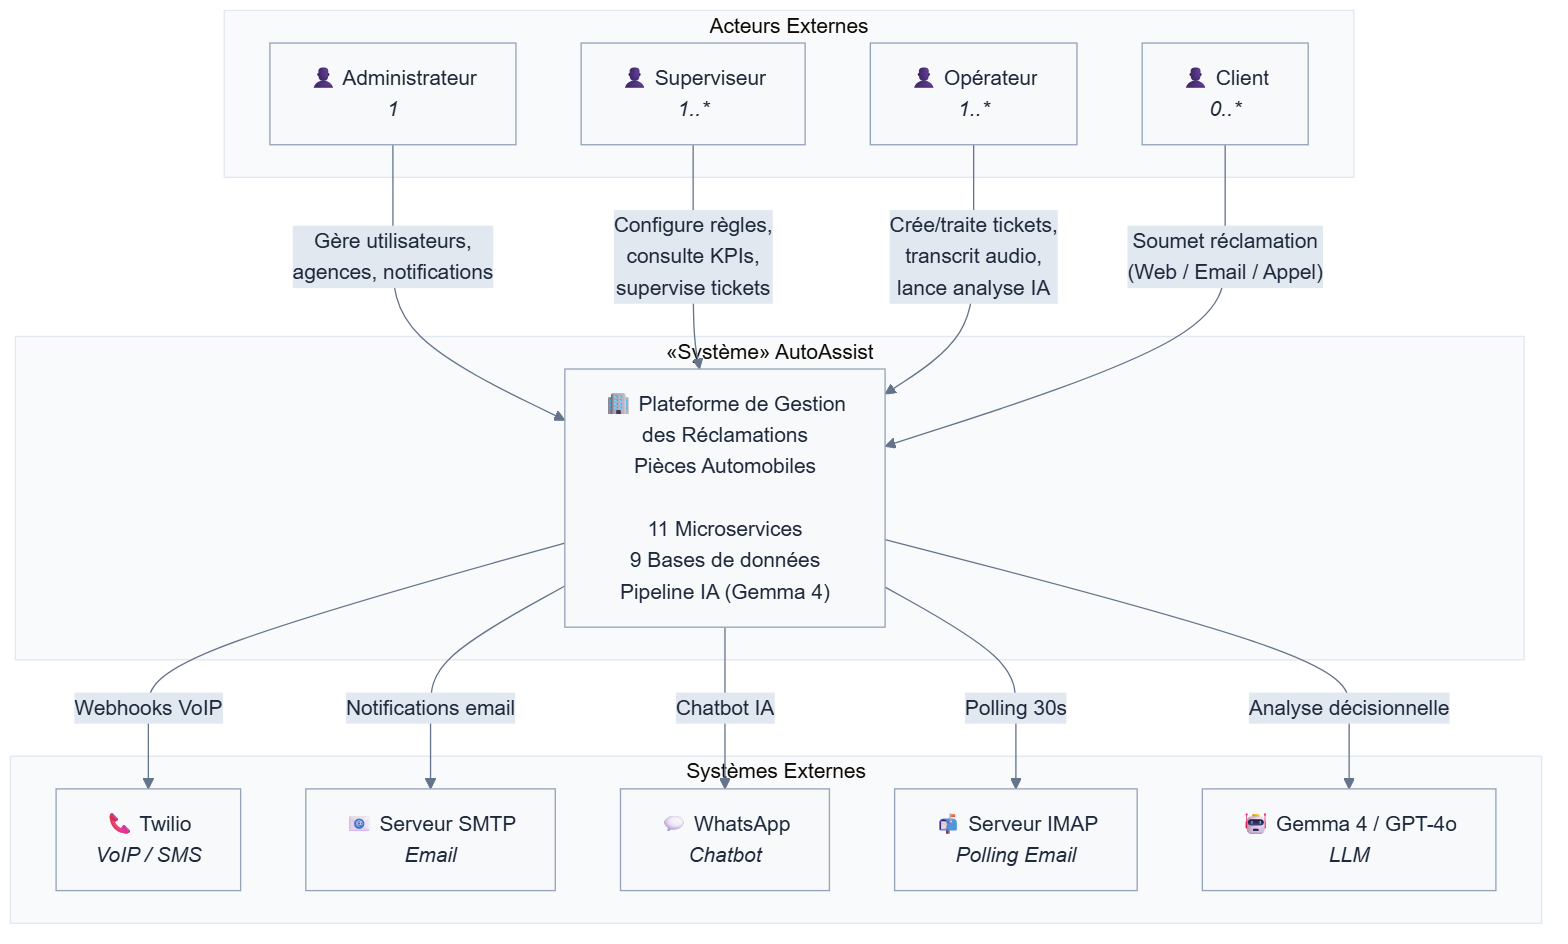
\includegraphics[width=0.95\textwidth]{figures_uml_finaux/00_diagramme_de_contexte_acteurs_systemes_externes.png}
    \caption{Diagramme de contexte du syst\`{e}me AutoAssist}
    \label{fig:contexte}
\end{figure}

\subsection{Diagrammes de cas d'utilisation}

Cette section pr\'{e}sente des diagrammes de cas d'utilisation, mettant en \'{e}vidence les diff\'{e}rentes interactions entre les utilisateurs et le syst\`{e}me.

\subsubsection{Diagramme de cas d'utilisation pour l'Administrateur et le Superviseur}

Le diagramme de cas d'utilisation, illustr\'{e} par la figure~\ref{fig:uc_admin}, met en \'{e}vidence les diff\'{e}rentes interactions possibles entre l'administrateur, le superviseur et le syst\`{e}me. Il offre une vue d'ensemble des actions que chaque acteur peut effectuer au sein de l'application, en fonction de son r\^{o}le.

\begin{figure}[htbp]
    \centering
    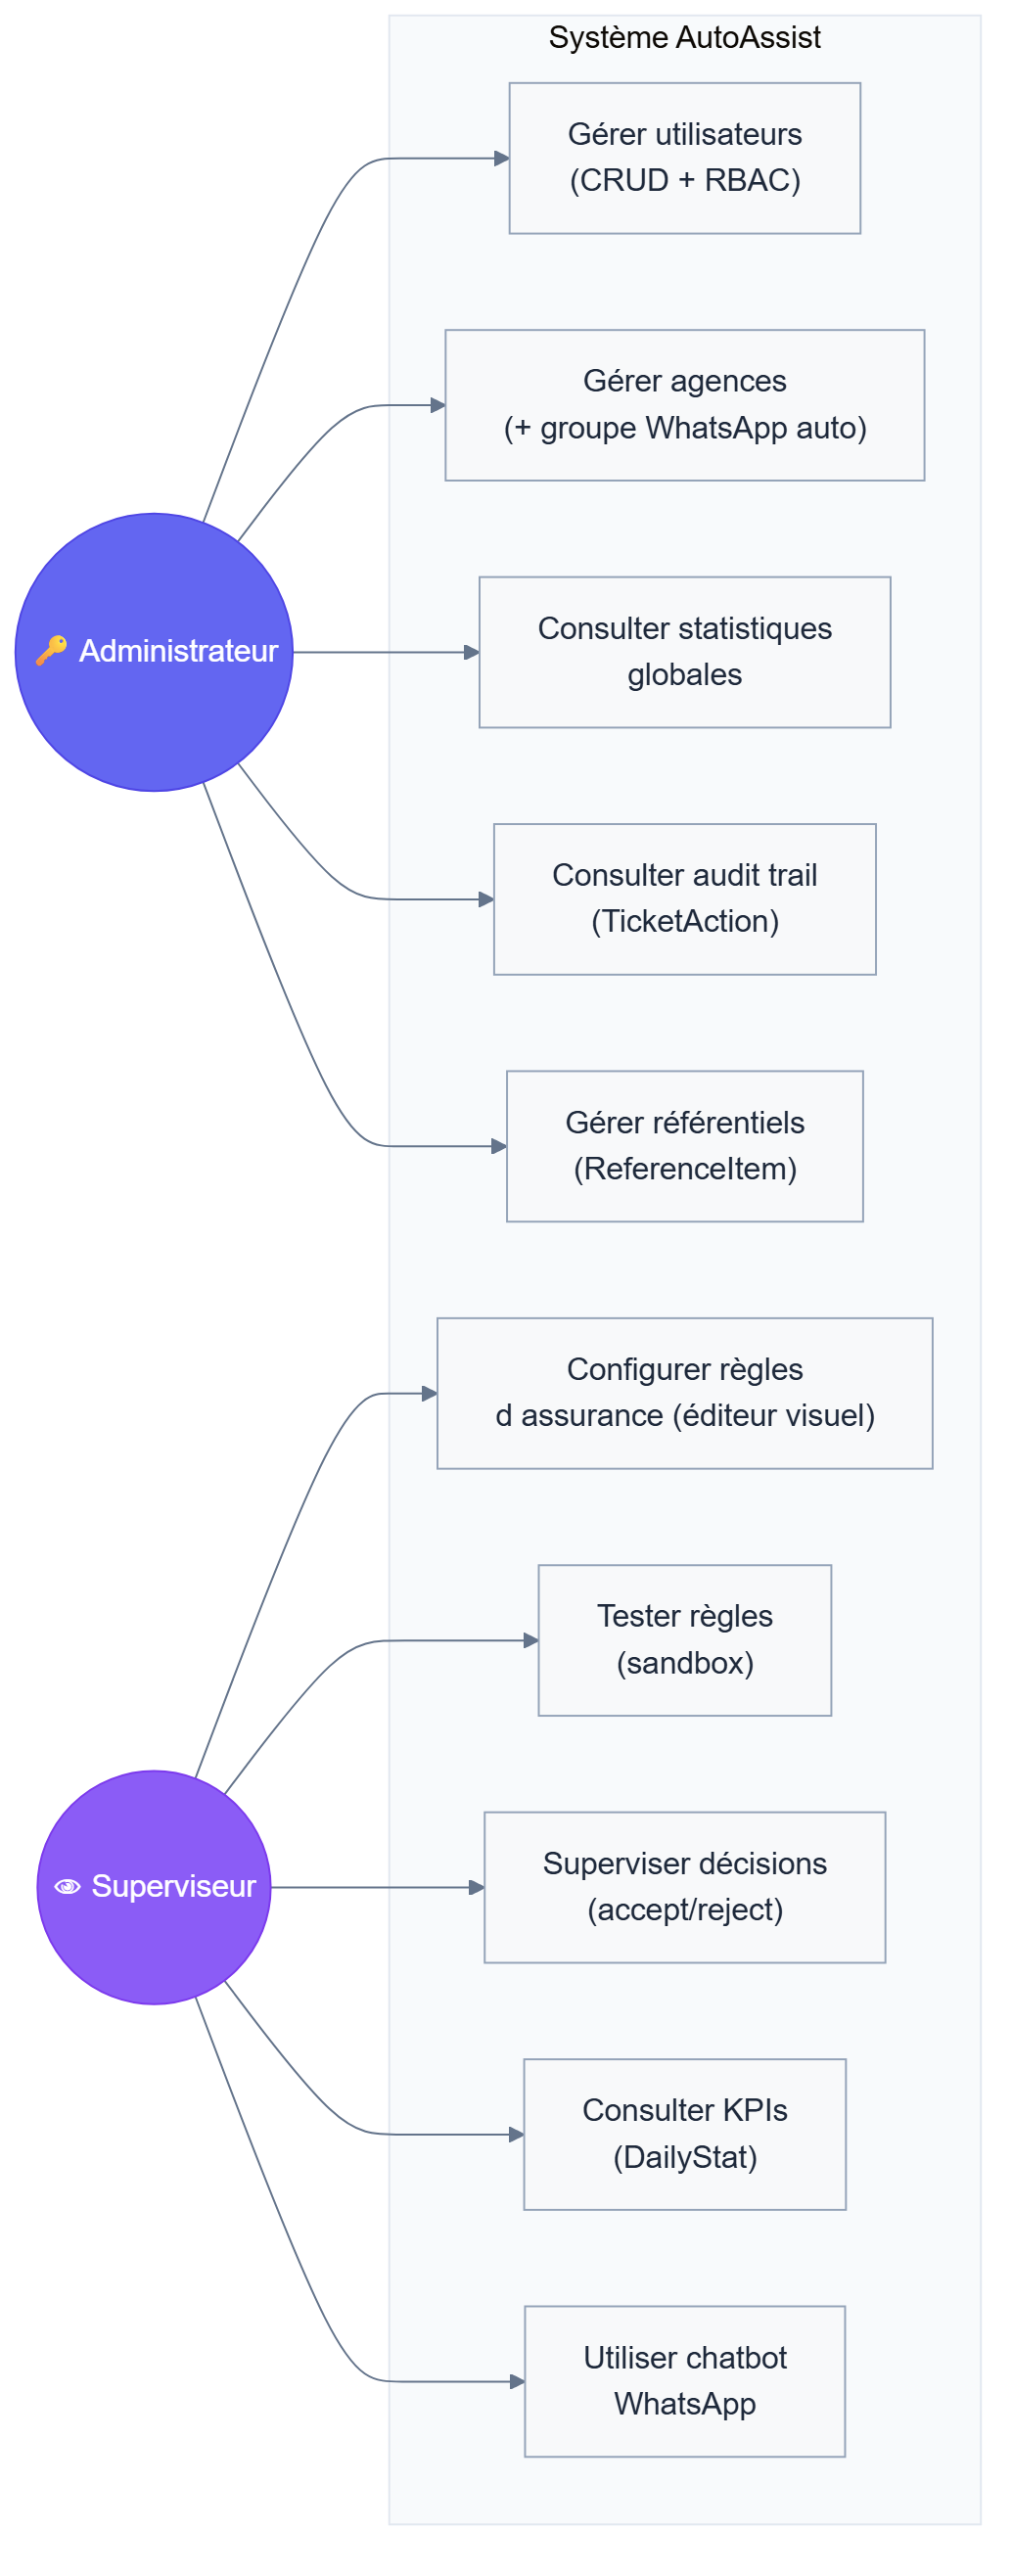
\includegraphics[height=0.78\textheight,keepaspectratio]{figures_uml_finaux/01_diagramme_de_cas_dutilisation_administrateur_superviseur.png}
    \caption{Diagramme de cas d'utilisation -- Administrateur et Superviseur}
    \label{fig:uc_admin}
\end{figure}

\subsubsection{Diagramme de cas d'utilisation pour l'Op\'{e}rateur}

Le diagramme de cas d'utilisation, illustr\'{e} par la figure~\ref{fig:uc_operator}, met en \'{e}vidence les diff\'{e}rentes interactions entre l'op\'{e}rateur et les fonctionnalit\'{e}s cl\'{e}s qui lui sont accessibles.

\begin{figure}[htbp]
    \centering
    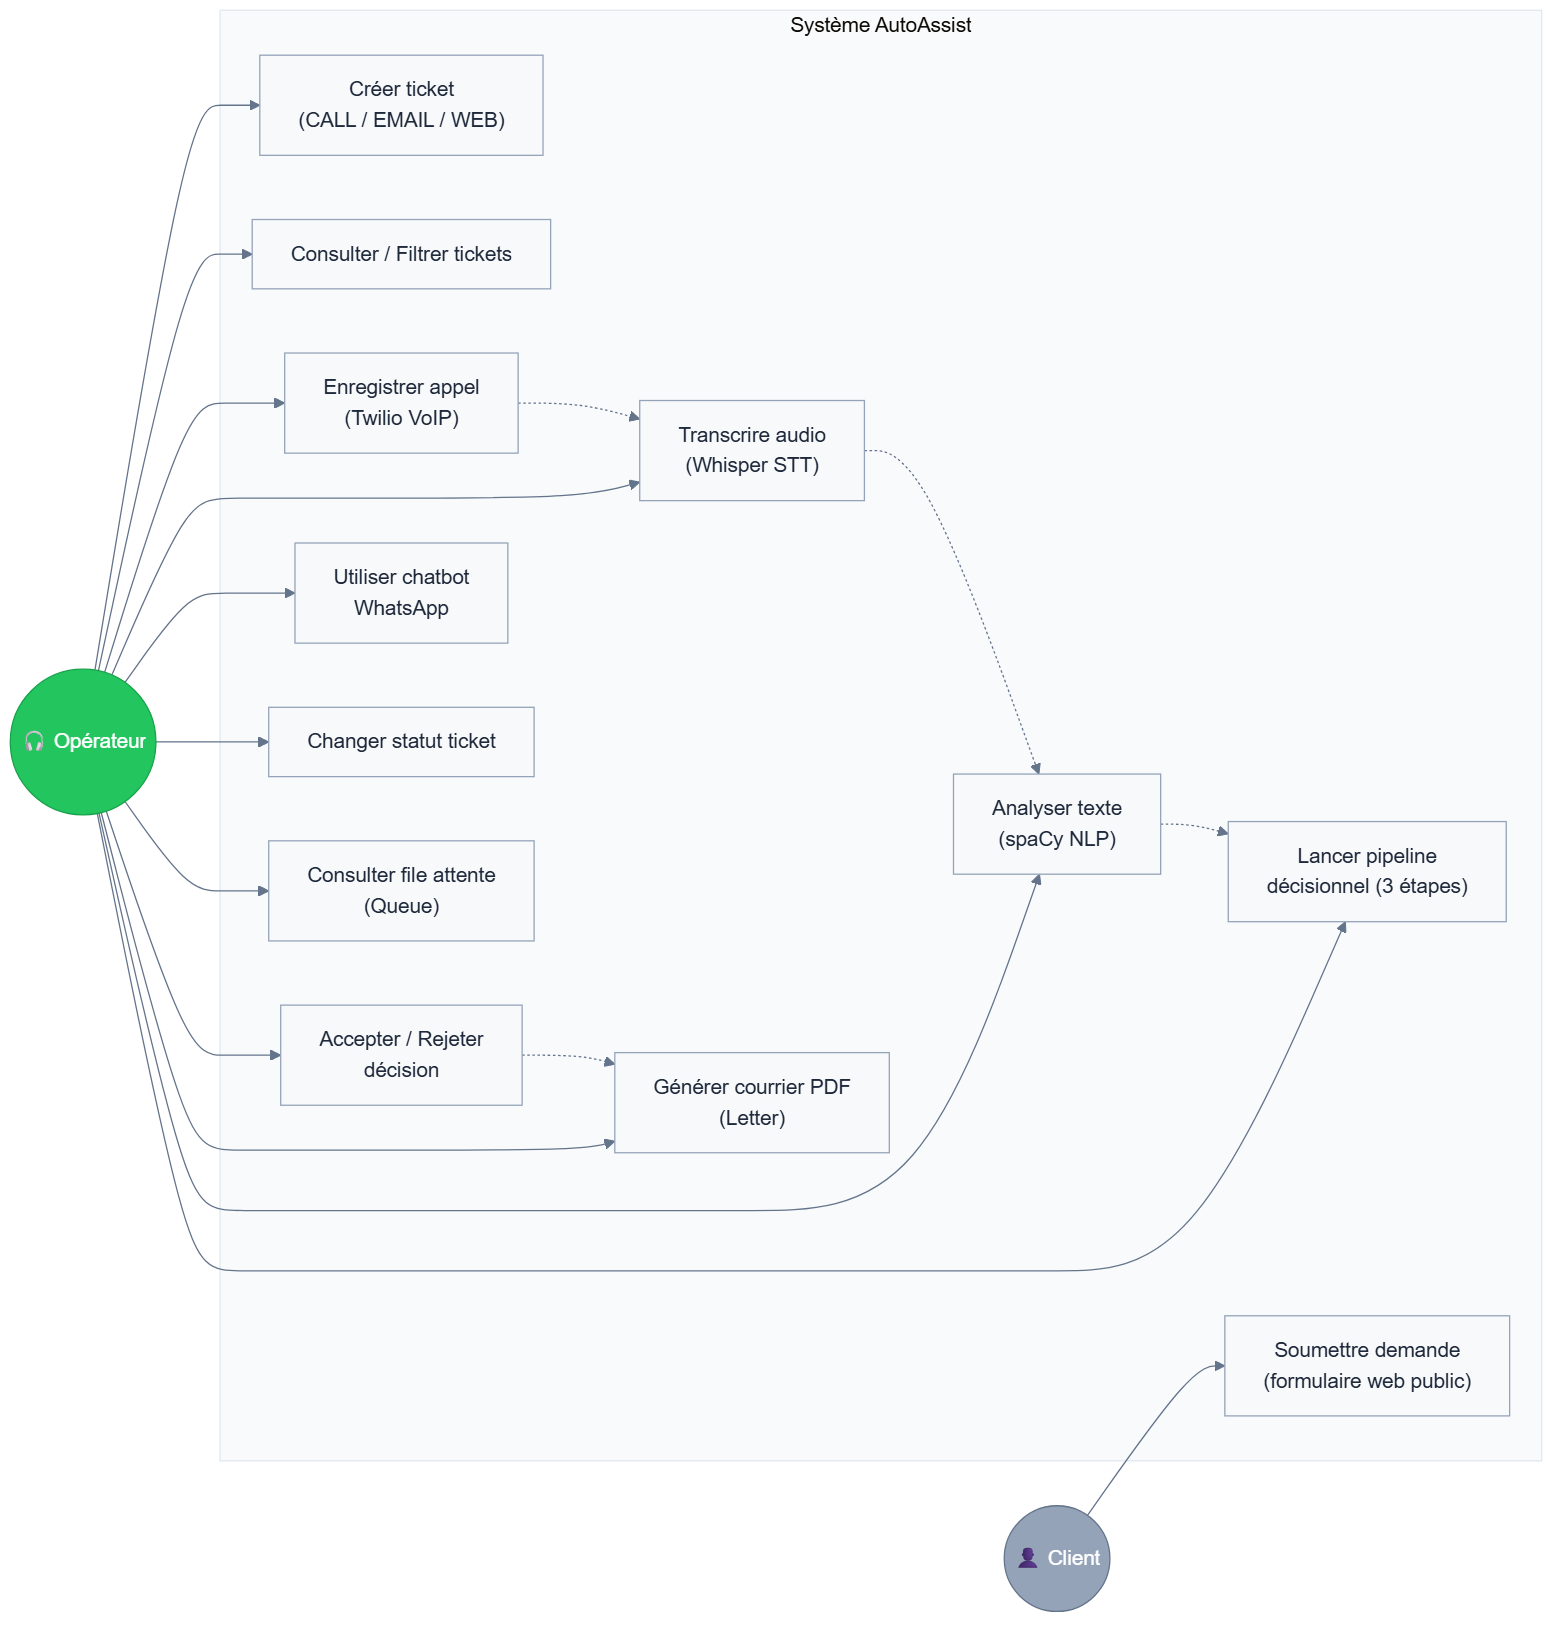
\includegraphics[width=\textwidth]{figures_uml_finaux/02_diagramme_de_cas_dutilisation_oprateur_client.png}
    \caption{Diagramme de cas d'utilisation -- Op\'{e}rateur}
    \label{fig:uc_operator}
\end{figure}

\subsubsection{Raffinement du cas d'utilisation \og Traiter un ticket avec aide IA \fg{}}

La figure~\ref{fig:uc_decision} pr\'{e}sente le diagramme de cas d'utilisation raffin\'{e} du cas d'utilisation \og Traiter un ticket avec aide IA \fg{}.

\begin{figure}[htbp]
    \centering
    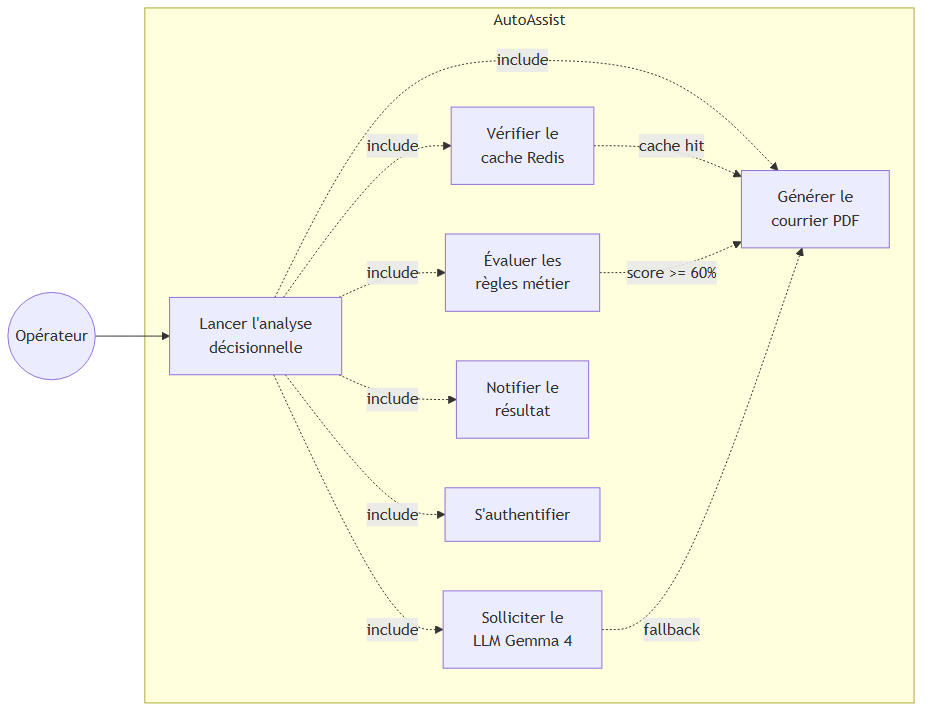
\includegraphics[width=0.80\textwidth]{figures/raffinement_decision.png}
    \caption{Raffinement du cas d'utilisation \og Traiter un ticket avec aide IA \fg{}}
    \label{fig:uc_decision}
\end{figure}

Le tableau~\ref{tab:uc_traiter} pr\'{e}sente la description textuelle du cas d'utilisation \og Traiter un ticket avec aide IA \fg{}.

\begin{table}[H]
\centering
\caption{Description textuelle du cas d'utilisation \og Traiter un ticket \fg{}}
\label{tab:uc_traiter}
\begin{tabular}{|p{3.5cm}|p{9.5cm}|}
\hline
\textbf{\'{E}l\'{e}ment} & \textbf{Description} \\
\hline
Cas d'utilisation & Traiter un ticket avec aide IA. \\
\hline
Acteur & Op\'{e}rateur \\
\hline
Objectif & Permettre \`{a} l'op\'{e}rateur de traiter une demande client en exploitant la transcription automatique, l'analyse NLP et le pipeline d\'{e}cisionnel hybride. \\
\hline
Pr\'{e}conditions & L'acteur doit \^{e}tre authentifi\'{e} dans l'application. Un ticket doit exister. \\
\hline
Postconditions & La d\'{e}cision est finalis\'{e}e, un courrier PDF est g\'{e}n\'{e}r\'{e} et le ticket est mis \`{a} jour. \\
\hline
Sc\'{e}nario nominal & 1. L'op\'{e}rateur s'authentifie sur l'application. \newline 2. Il ouvre le d\'{e}tail du ticket. \newline 3. Il uploade l'enregistrement audio. \newline 4. Whisper transcrit et spaCy analyse~: \newline \hspace{0.5cm} -- Extraction des mots-cl\'{e}s. \newline \hspace{0.5cm} -- D\'{e}tection du type de sinistre. \newline \hspace{0.5cm} -- Analyse du sentiment. \newline 5. Le formulaire est pr\'{e}-rempli. \newline 6. L'op\'{e}rateur lance l'analyse d\'{e}cisionnelle. \newline 7. Il accepte ou rejette la recommandation. \\
\hline
\end{tabular}
\end{table}

\subsubsection{Raffinement du cas d'utilisation \og Interroger le chatbot WhatsApp \fg{}}

La figure~\ref{fig:uc_chatbot} pr\'{e}sente le diagramme de cas d'utilisation raffin\'{e} du cas d'utilisation \og Interroger le chatbot WhatsApp \fg{}.

\begin{figure}[htbp]
    \centering
    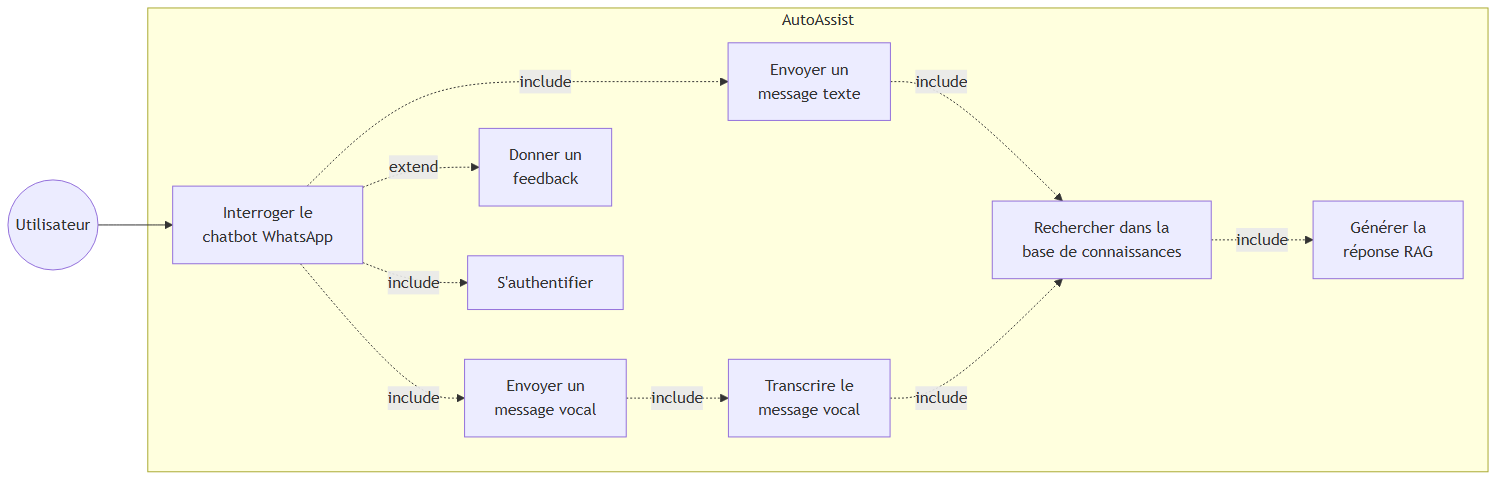
\includegraphics[width=\textwidth]{figures/raffinement_chatbot.png}
    \caption{Raffinement du cas d'utilisation \og Interroger le chatbot \fg{}}
    \label{fig:uc_chatbot}
\end{figure}

\begin{table}[H]
\centering
\caption{Description textuelle du cas d'utilisation \og Interroger le chatbot \fg{}}
\label{tab:uc_chatbot}
\begin{tabular}{|p{3.5cm}|p{9.5cm}|}
\hline
\textbf{\'{E}l\'{e}ment} & \textbf{Description} \\
\hline
Cas d'utilisation & Interroger le chatbot WhatsApp. \\
\hline
Acteur & Op\'{e}rateur / Superviseur \\
\hline
Objectif & Permettre aux utilisateurs d'obtenir des r\'{e}ponses pr\'{e}cises sur les proc\'{e}dures internes et les r\`{e}gles m\'{e}tier via un chatbot intelligent. \\
\hline
Pr\'{e}conditions & L'acteur doit \^{e}tre authentifi\'{e}. Le service RAG doit \^{e}tre op\'{e}rationnel. \\
\hline
Postconditions & Une r\'{e}ponse pertinente est envoy\'{e}e \`{a} l'utilisateur via WhatsApp. \\
\hline
Sc\'{e}nario nominal & 1. L'utilisateur envoie un message (texte ou vocal). \newline 2. Le syst\`{e}me identifie le type de message~: \newline \hspace{0.5cm} -- Message texte~: recherche hybride ChromaDB. \newline \hspace{0.5cm} -- Message vocal~: transcription Whisper puis RAG. \newline \hspace{0.5cm} -- Commande rapide~: ex\'{e}cution API directe. \newline 3. Le syst\`{e}me g\'{e}n\`{e}re et envoie la r\'{e}ponse. \\
\hline
\end{tabular}
\end{table}

\subsubsection{Raffinement du cas d'utilisation \og Configurer les r\`{e}gles d'assurance \fg{}}

La figure~\ref{fig:uc_rules_raff} pr\'{e}sente le diagramme de cas d'utilisation raffin\'{e} du cas d'utilisation \og Configurer les r\`{e}gles d'assurance \fg{}.

\begin{figure}[htbp]
    \centering
    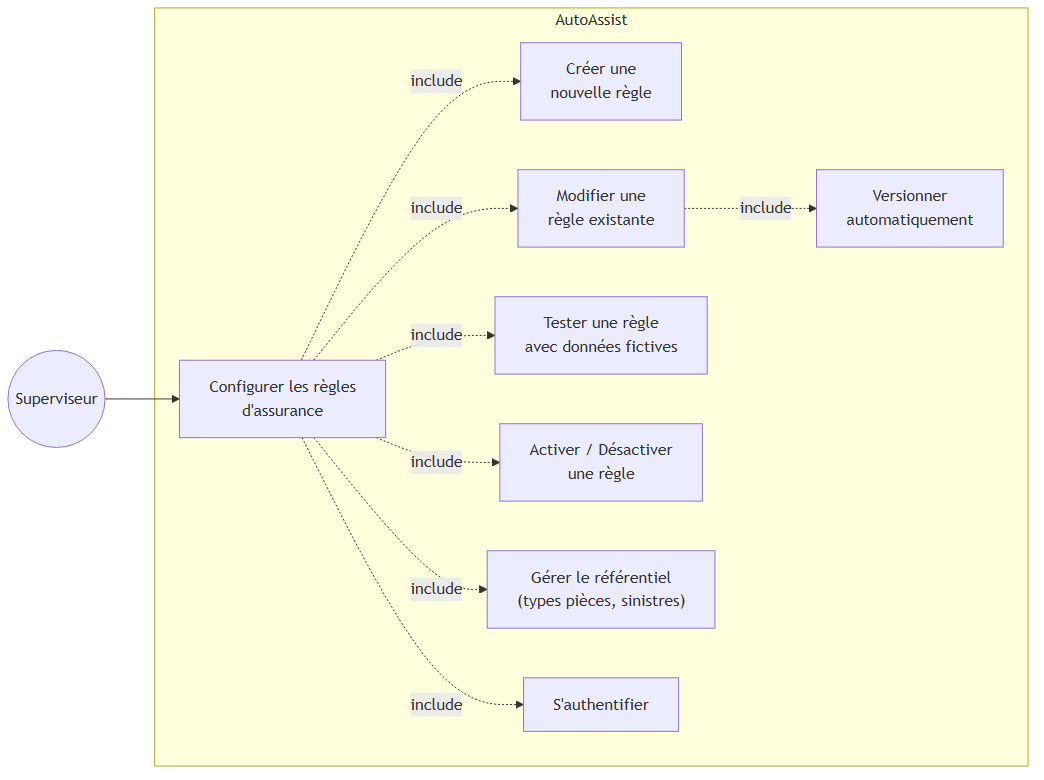
\includegraphics[width=0.80\textwidth]{figures/raffinement_rules.png}
    \caption{Raffinement du cas d'utilisation \og Configurer les r\`{e}gles \fg{}}
    \label{fig:uc_rules_raff}
\end{figure}

\begin{table}[H]
\centering
\caption{Description textuelle du cas d'utilisation \og Configurer les r\`{e}gles \fg{}}
\label{tab:uc_rules}
\begin{tabular}{|p{3.5cm}|p{9.5cm}|}
\hline
\textbf{\'{E}l\'{e}ment} & \textbf{Description} \\
\hline
Cas d'utilisation & Configurer les r\`{e}gles d'assurance. \\
\hline
Acteur & Superviseur \\
\hline
Objectif & Permettre au superviseur de cr\'{e}er, modifier et tester des r\`{e}gles d'assurance via un \'{e}diteur visuel, incluant le versioning. \\
\hline
Pr\'{e}conditions & L'acteur doit \^{e}tre authentifi\'{e} dans l'application. \\
\hline
Postconditions & Les r\`{e}gles sont cr\'{e}\'{e}es, modifi\'{e}es ou activ\'{e}es selon les actions r\'{e}alis\'{e}es. L'historique de versioning est mis \`{a} jour. \\
\hline
Sc\'{e}nario nominal & 1. Le superviseur s'authentifie sur l'application. \newline 2. Il acc\`{e}de \`{a} l'\'{e}diteur visuel de r\`{e}gles. \newline 3. Il peut~: \newline \hspace{0.5cm} -- Cr\'{e}er une nouvelle r\`{e}gle (conditions JSONB). \newline \hspace{0.5cm} -- Modifier une r\`{e}gle existante. \newline \hspace{0.5cm} -- Tester avec des donn\'{e}es fictives. \newline \hspace{0.5cm} -- Activer ou d\'{e}sactiver une r\`{e}gle. \newline 4. Le syst\`{e}me enregistre et versionne la r\`{e}gle. \\
\hline
\end{tabular}
\end{table}

\section{Cadre m\'{e}thodologique}
\label{sec:cadre}

\subsection{M\'{e}thodologie de d\'{e}veloppement~: Scrum}

Une m\'{e}thodologie de d\'{e}veloppement logiciel d\'{e}finit les diff\'{e}rentes \'{e}tapes et s\'{e}quences dans le processus de r\'{e}alisation d'une application. Face \`{a} la complexit\'{e} croissante des projets informatiques et \`{a} la n\'{e}cessit\'{e} de s'adapter rapidement aux \'{e}volutions des besoins, les approches agiles se sont impos\'{e}es comme une alternative plus flexible aux m\'{e}thodes traditionnelles de gestion de projet.

\indent Parmi les m\'{e}thodes de d\'{e}veloppement classiques, le \textbf{cycle en V} garantit une documentation exhaustive et une tra\c{c}abilit\'{e} rigoureuse des exigences, mais il pr\'{e}sente l'inconv\'{e}nient majeur de livrer le produit final en une seule fois, \`{a} la fin du projet. Toute erreur de conception d\'{e}tect\'{e}e tardivement engendre alors un co\^{u}t de correction \'{e}lev\'{e}. De m\^{e}me, \textbf{Kanban} offre une gestion visuelle efficace du flux de t\^{a}ches, mais sans cadre temporel d\'{e}fini ni m\'{e}canisme de planification des incr\'{e}ments fonctionnels.

\indent \textbf{Scrum}, en revanche, est un cadre de travail agile qui permet de relever ces d\'{e}fis en organisant le d\'{e}veloppement autour de cycles courts et it\'{e}ratifs appel\'{e}s \textit{sprints} \cite{scrum}. Il repose sur trois piliers fondamentaux~: la \textbf{transparence}, qui impose que les aspects significatifs du processus soient visibles de tous les acteurs concern\'{e}s~; l'\textbf{inspection}, qui exige une \'{e}valuation fr\'{e}quente des artefacts et de la progression vers les objectifs~; et l'\textbf{adaptation}, qui permet d'ajuster le processus d\`{e}s qu'un \'{e}cart est d\'{e}tect\'{e}.

\indent Chaque sprint, d'une dur\'{e}e fixe de deux \`{a} quatre semaines, comprend une phase de planification (\textit{Sprint Planning}), des r\'{e}unions quotidiennes de synchronisation (\textit{Daily Scrum}), une revue des fonctionnalit\'{e}s livr\'{e}es (\textit{Sprint Review}) et une r\'{e}trospective collective (\textit{Sprint Retrospective}).

\indent \textbf{Justification du choix de Scrum pour AutoAssist.} Le projet AutoAssist pr\'{e}sente plusieurs caract\'{e}ristiques qui rendent Scrum particuli\`{e}rement adapt\'{e}. D'une part, la complexit\'{e} technique est \'{e}lev\'{e}e~: onze microservices ind\'{e}pendants, trois langages de programmation (Java, Python, Dart) et plusieurs technologies d'IA (Whisper, spaCy, Gemma~4, RAG) impliquent des interd\'{e}pendances nombreuses qu'il est pr\'{e}f\'{e}rable de valider par it\'{e}rations successives plut\^{o}t que de sp\'{e}cifier exhaustivement en amont. D'autre part, certaines fonctionnalit\'{e}s --- notamment le pipeline d\'{e}cisionnel hybride et le chatbot WhatsApp --- n\'{e}cessitent des retours utilisateur r\'{e}guliers pour affiner les param\`{e}tres des mod\`{e}les IA et les seuils de d\'{e}cision. Enfin, la m\'{e}thode Scrum facilite la communication entre l'\'{e}quipe de d\'{e}veloppement et les parties prenantes m\'{e}tier, garantissant un alignement continu entre les fonctionnalit\'{e}s livr\'{e}es et les besoins r\'{e}els du terrain.

\subsection{Pilotage du projet par Scrum}

Pour le projet AutoAssist, les r\^{o}les Scrum sont attribu\'{e}s comme suit~:

\begin{itemize}[label=---]
    \item \textbf{M. Nezar Torche~:} Il occupe le r\^{o}le de Product Owner. En tant que principal point de contact au sein de l'entreprise, il d\'{e}finit les besoins et priorit\'{e}s du projet, g\`{e}re le Product Backlog et valide les livrables.
    \item \textbf{Mme Hedia Selmi~:} Elle joue le r\^{o}le de Scrum Master. En tant qu'encadreur professionnel, elle veille \`{a} la bonne application de la d\'{e}marche Scrum, facilite les r\'{e}unions et aide \`{a} la r\'{e}solution des obstacles rencontr\'{e}s par l'\'{e}quipe.
    \item \textbf{Rezgui Seif Eddine~:} Il joue le r\^{o}le d'un membre de l'\'{E}quipe de D\'{e}veloppement. Responsable de l'ex\'{e}cution des t\^{a}ches, du d\'{e}veloppement des fonctionnalit\'{e}s et de la livraison des incr\'{e}ments du produit \`{a} la fin de chaque Sprint. Il assure la conception, la r\'{e}alisation technique et la qualit\'{e} des fonctionnalit\'{e}s d\'{e}velopp\'{e}es.
\end{itemize}

\subsection{Backlog du produit}

Cette section met en lumi\`{e}re l'\'{e}l\'{e}ment central de la planification~: le backlog produit. Le tableau~\ref{tab:backlog} en pr\'{e}sente une version structur\'{e}e, regroupant l'ensemble des fonctionnalit\'{e}s dans notre projet.

\begin{longtable}{|c|p{2.5cm}|c|p{5.8cm}|c|}
\caption{Backlog du produit} \label{tab:backlog} \\
\hline
\textbf{ID-F} & \textbf{Features} & \textbf{ID-Us} & \textbf{User Stories} & \textbf{Priorit\'{e}} \\
\hline
\endfirsthead
\hline \textbf{ID-F} & \textbf{Features} & \textbf{ID-Us} & \textbf{User Stories} & \textbf{Priorit\'{e}} \\ \hline
\endhead
\multirow{2}{*}{1} & \multirow{2}{2.8cm}{Authentification} & 1.1 & En tant qu'utilisateur, je souhaite m'authentifier afin d'acc\'{e}der \`{a} la plateforme. & Haute \\
\cline{3-5}
 & & 1.2 & En tant qu'utilisateur, je souhaite pouvoir me d\'{e}connecter pour s\'{e}curiser mon compte. & Moyenne \\
\hline
\multirow{3}{*}{2} & \multirow{3}{2.8cm}{Gestion des utilisateurs et agences} & 2.1 & En tant qu'admin, je souhaite g\'{e}rer les utilisateurs en cr\'{e}ant des comptes et en attribuant les r\^{o}les. & Haute \\
\cline{3-5}
 & & 2.2 & En tant qu'admin, je souhaite g\'{e}rer les agences afin d'organiser la structure de l'entreprise. & Haute \\
\cline{3-5}
 & & 2.3 & En tant qu'utilisateur, je souhaite consulter et modifier mon profil. & Moyenne \\
\hline
\multirow{3}{*}{3} & \multirow{3}{2.8cm}{Gestion des tickets} & 3.1 & En tant qu'op\'{e}rateur, je souhaite cr\'{e}er un ticket \`{a} partir d'un appel, email ou formulaire. & Haute \\
\cline{3-5}
 & & 3.2 & En tant qu'op\'{e}rateur, je souhaite suivre le cycle de vie d'un ticket en temps r\'{e}el. & Haute \\
\cline{3-5}
 & & 3.3 & En tant que client, je souhaite soumettre ma demande via un formulaire web. & Moyenne \\
\hline
\multirow{2}{*}{4} & \multirow{2}{2.8cm}{Transcription et analyse IA} & 4.1 & En tant qu'op\'{e}rateur, je souhaite transcrire un enregistrement audio afin d'obtenir le texte de l'appel. & Haute \\
\cline{3-5}
 & & 4.2 & En tant que syst\`{e}me, je souhaite pr\'{e}-remplir le formulaire avec les donn\'{e}es extraites par NLP. & Haute \\
\hline
\multirow{2}{*}{5} & \multirow{2}{2.8cm}{Pipeline d\'{e}cisionnel} & 5.1 & En tant qu'op\'{e}rateur, je souhaite lancer l'analyse d\'{e}cisionnelle afin d'obtenir une recommandation. & Haute \\
\cline{3-5}
 & & 5.2 & En tant qu'op\'{e}rateur, je souhaite g\'{e}n\'{e}rer un courrier PDF apr\`{e}s la d\'{e}cision. & Haute \\
\hline
\multirow{2}{*}{6} & \multirow{2}{2.8cm}{Chatbot WhatsApp} & 6.1 & En tant qu'utilisateur, je souhaite interroger le chatbot sur les proc\'{e}dures internes. & Haute \\
\cline{3-5}
 & & 6.2 & En tant qu'utilisateur, je souhaite envoyer un message vocal au chatbot. & Moyenne \\
\hline
7 & R\`{e}gles m\'{e}tier & 7.1 & En tant que superviseur, je souhaite configurer les r\`{e}gles d'assurance via un \'{e}diteur visuel. & Haute \\
\hline
8 & Analytics & 8.1 & En tant que superviseur, je souhaite consulter les KPIs et tableaux de bord. & Moyenne \\
\hline
9 & Mobile & 9.1 & En tant qu'op\'{e}rateur, je souhaite g\'{e}rer les tickets depuis l'application mobile. & Basse \\
\hline
\end{longtable}

\subsection{Planification du projet avec sprints}

La planification des sprints constitue une \'{e}tape cl\'{e} dans l'organisation du d\'{e}veloppement du projet selon la m\'{e}thodologie Scrum. Pour garantir une progression structur\'{e}e et ma\^{i}tris\'{e}e, le projet a \'{e}t\'{e} d\'{e}coup\'{e} en six sprints successifs. Chaque sprint cible un ensemble coh\'{e}rent de fonctionnalit\'{e}s.

\indent Le d\'{e}coupage du projet se fait comme suit~:

\begin{table}[H]
\centering
\caption{Planification des sprints}
\label{tab:sprints}
\small
\begin{tabular}{|c|c|p{7cm}|c|}
\hline
\textbf{Sprint} & \textbf{Dur\'{e}e} & \textbf{Objectifs} & \textbf{ID-Us} \\
\hline
Sprint 0 & 3 sem. & Infrastructure, CI/CD et authentification & 1.1, 1.2 \\
\hline
Sprint 1 & 3 sem. & Organisations, tickets et canaux d'acquisition & 2.1--3.3 \\
\hline
Sprint 2 & 3 sem. & Service IA (transcription, NLP) et frontend & 4.1, 4.2 \\
\hline
Sprint 3 & 3 sem. & Moteur de r\`{e}gles, pipeline d\'{e}cisionnel, PDF & 5.1, 5.2, 7.1 \\
\hline
Sprint 4 & 3 sem. & Chatbot WhatsApp RAG et analytics & 6.1, 6.2, 8.1 \\
\hline
Sprint 5 & 2 sem. & Application mobile Flutter et tests & 9.1 \\
\hline
\end{tabular}
\end{table}

\section*{Conclusion}
\label{sec:conclusion}

Ce chapitre a permis d'analyser les besoins du projet, d'identifier les diff\'{e}rents acteurs, ainsi que de sp\'{e}cifier les besoins fonctionnels et non fonctionnels. Ces \'{e}l\'{e}ments ont \'{e}t\'{e} mod\'{e}lis\'{e}s \`{a} travers des diagrammes UML. La m\'{e}thodologie Scrum a structur\'{e} la planification en sprints pour une gestion agile et efficace. Le chapitre suivant se penchera sur la conception de la solution.


\chapter{Conception}
\label{chap:conception}

\vspace{2cm}

\noindent\textbf{\Large Plan}

\vspace{0.5cm}
\noindent\rule{\textwidth}{0.4pt}
\vspace{0.3cm}

\begin{list}{}{\setlength{\leftmargin}{1.5cm}\setlength{\itemsep}{6pt}}
  \item \textbf{1} \hspace{0.3cm} Architecture du syst\`{e}me \dotfill \pageref{sec:architecture}
  \item \textbf{2} \hspace{0.3cm} Conception d\'{e}taill\'{e}e \dotfill \pageref{sec:conception_detail}
  \item \textbf{3} \hspace{0.3cm} Conclusion \dotfill \pageref{sec:conclusion_ch2}
\end{list}

\vspace{0.3cm}
\noindent\rule{\textwidth}{0.4pt}

\newpage

\section*{Introduction}

Ce chapitre pr\'{e}sente la conception technique du syst\`{e}me AutoAssist. Nous commencerons par d\'{e}crire l'architecture globale du syst\`{e}me, puis nous d\'{e}taillerons la conception via les vues statique (diagrammes de classes) et dynamique (diagrammes de s\'{e}quence).

%% ═══════════════════════════════════════════════════
%% 2.1 ARCHITECTURE
%% (Réf: 2.1 Architecture physique)
%% ═══════════════════════════════════════════════════
\section{Architecture du système}
\label{sec:architecture}

\subsection{Architecture physique}

Le syst\`{e}me AutoAssist est d\'{e}ploy\'{e} sous forme de 17 conteneurs Docker \cite{docker} orchestr\'{e}s via Docker Compose, r\'{e}partis en cinq couches~:

\begin{figure}[htbp]
    \centering
    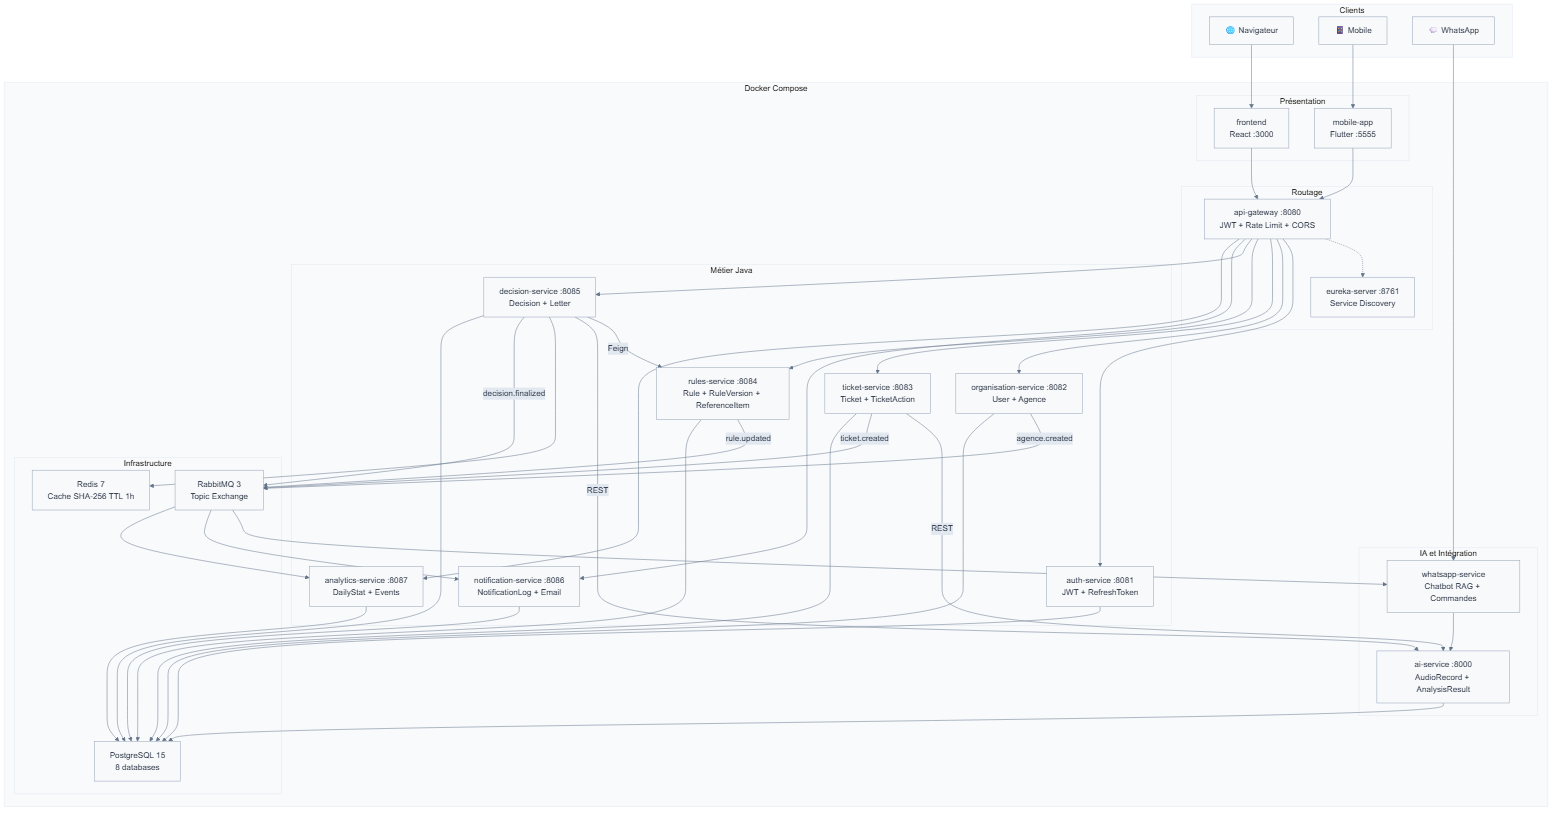
\includegraphics[width=\textwidth]{figures_uml_finaux/06_diagramme_de_dploiement_architecture_docker_14_conteneurs.png}
    \caption{Architecture physique du système AutoAssist}
    \label{fig:archi_physique}
\end{figure}

\begin{table}[H]
\centering
\caption{Conteneurs Docker du système AutoAssist}
\label{tab:conteneurs}
\begin{tabular}{|p{3.5cm}|p{3cm}|c|p{4cm}|}
\hline
\textbf{Service} & \textbf{Technologie} & \textbf{Port} & \textbf{Base de données} \\
\hline
\multicolumn{4}{|c|}{\textit{Couche Infrastructure}} \\
\hline
postgres & PostgreSQL 15 & 5432 & 8 bases (multi-tenant) \\
\hline
redis & Redis 7 & 6379 & Cache décisions \\
\hline
rabbitmq & RabbitMQ 3 & 5672 & Files de messages \\
\hline
\multicolumn{4}{|c|}{\textit{Couche Découverte et Routage}} \\
\hline
eureka-server & Spring Cloud & 8761 & -- \\
\hline
api-gateway & Spring Cloud Gateway & 8080 & Redis (rate limiting) \\
\hline
\multicolumn{4}{|c|}{\textit{Couche Services Métier (Java / Spring Boot 3)}} \\
\hline
auth-service & Java 21 & 8081 & auth\_db \\
\hline
organisation-service & Java 21 & 8082 & users\_db \\
\hline
ticket-service & Java 21 & 8083 & tickets\_db \\
\hline
rules-service & Java 21 & 8084 & rules\_db \\
\hline
decision-service & Java 21 & 8085 & decisions\_db \\
\hline
notification-service & Java 21 & 8086 & notif\_db \\
\hline
analytics-service & Java 21 & 8087 & analytics\_db \\
\hline
\multicolumn{4}{|c|}{\textit{Couche IA et Intégration}} \\
\hline
ai-service & Python FastAPI & 8000 & ai\_db + ChromaDB \\
\hline
whatsapp-service & Node.js & -- & ai\_db (RAG feedback) \\
\hline
\multicolumn{4}{|c|}{\textit{Couche Présentation}} \\
\hline
frontend & React 18 / Vite & 3000 & -- \\
\hline
mobile-app & Flutter Web & 5555 & -- \\
\hline
\end{tabular}
\end{table}

\subsection{Architecture logique}

L'architecture logique suit le patron microservices avec les principes suivants~:

\begin{itemize}
    \item \textbf{Service Discovery}~: chaque service s'enregistre auprès d'Eureka Server au démarrage. Le gateway résout les routes dynamiquement~;
    \item \textbf{Communication synchrone}~: via REST (OpenFeign pour les appels inter-services Java, HTTP pour les appels vers ai-service Python)~;
    \item \textbf{Communication asynchrone}~: via RabbitMQ (événements \texttt{ticket.created}, \texttt{decision.finalized}, \texttt{agence.created})~;
    \item \textbf{S\'{e}curit\'{e}}~: le gateway valide le JWT sur chaque requ\^{e}te entrante. Les services internes communiquent sur le r\'{e}seau Docker isol\'{e}. En perspective, l'ajout de mTLS (mutual TLS) ou d'un service mesh est envisag\'{e} pour renforcer la s\'{e}curit\'{e} inter-services en production~;
    \item \textbf{Cache}~: Redis stocke les décisions calculées (clé SHA-256, TTL 1h) pour éviter les recalculs coûteux~;
    \item \textbf{Résilience}~: Circuit Breaker Resilience4j sur l'appel au LLM Gemma~4, avec fallback automatique vers la décision ETUDE (source CIRCUIT\_BREAKER).
\end{itemize}

\begin{figure}[htbp]
    \centering
    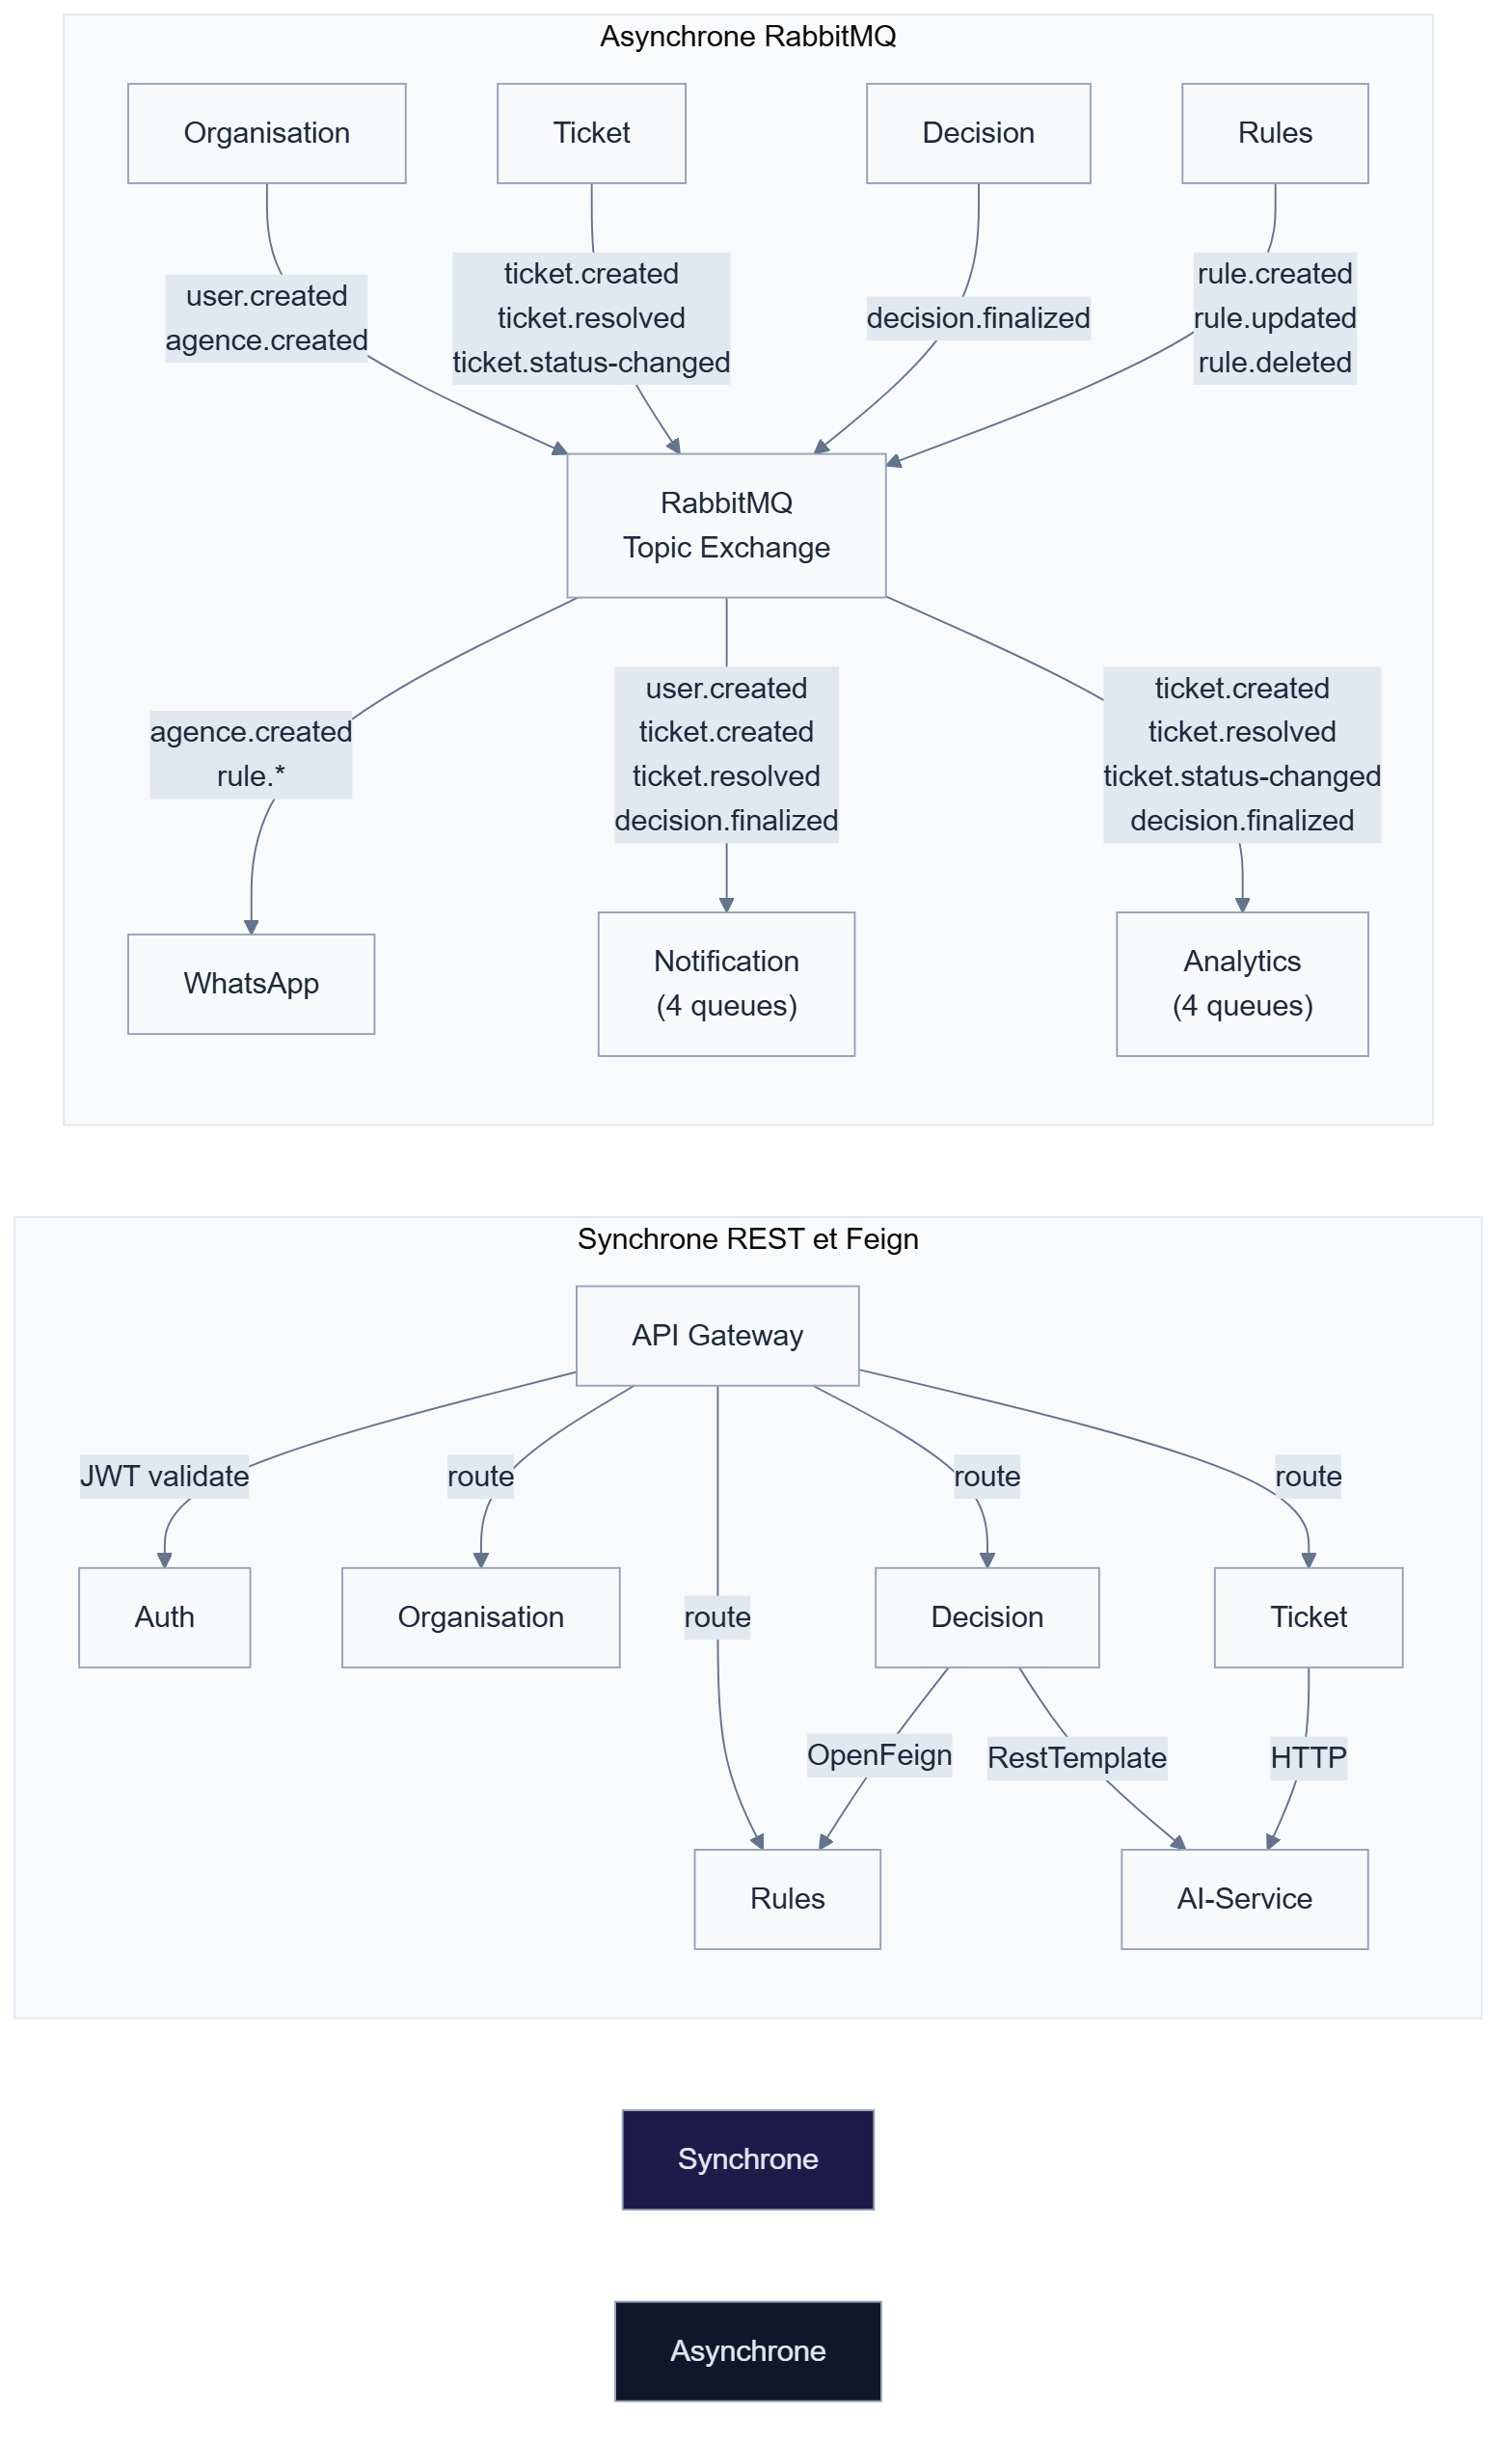
\includegraphics[width=0.95\textwidth]{figures_uml_finaux/07_diagramme_de_composants_communication_synchrone_vs_asynchrone.png}
    \caption{Architecture logique du système AutoAssist}
    \label{fig:archi_logique}
\end{figure}

\subsection{Architecture du pipeline d'aide à la décision}

Le pipeline de décision est l'innovation principale du système. Il évalue chaque demande en trois étapes successives~:

Le flux d\'{e}taill\'{e} de ce pipeline est illustr\'{e} par le diagramme de s\'{e}quence de la figure~\ref{fig:seq_decision} (section~\ref{sec:conception_detail}).

\begin{enumerate}
    \item \textbf{Étape 1 — Cache Redis}~: calcul d'un hash SHA-256 à partir des paramètres (typePiece, ageVehicule, kilometrage, categorieClient, typeSinistre). Si un résultat identique existe en cache (TTL = 3600s), il est retourné immédiatement ($<$ 50ms)~;
    \item \textbf{\'{E}tape 2 --- Moteur de r\`{e}gles}~: appel Feign vers le rules-service. Les r\`{e}gles JSONB actives sont \'{e}valu\'{e}es avec un score. Si le score $\geq$ 60\% et la d\'{e}cision n'est pas ambigu\"e, elle est retourn\'{e}e ($<$ 2s). Si le score est entre 40\% et 60\%, le cas est consid\'{e}r\'{e} ambigu et bascule vers l'\'{e}tape 3. Si le score est inf\'{e}rieur \`{a} 40\%, la d\'{e}cision est REFUS\'{E}E~;
    \item \textbf{\'{E}tape 3 --- LLM Gemma~4}~: pour les cas ambigus (score entre 40\% et 60\%), le mod\`{e}le local est sollicit\'{e} via Docker Model Runner. Un prompt structur\'{e} demande un JSON \{decision, score, motif\}. Un Circuit Breaker Resilience4j prot\`{e}ge contre les timeouts ($<$ 12s). En cas d'\'{e}chec du LLM, le syst\`{e}me retourne automatiquement une d\'{e}cision \'{E}TUDE avec la source CIRCUIT\_BREAKER.
\end{enumerate}

\subsection{Architecture du chatbot RAG}

Le chatbot WhatsApp utilise une architecture RAG (Retrieval-Augmented Generation) avec huit améliorations~:

Le flux d\'{e}taill\'{e} est pr\'{e}sent\'{e} dans le diagramme de s\'{e}quence de la figure~\ref{fig:seq_chatbot} (section~\ref{sec:conception_detail}).

\begin{table}[H]
\centering
\caption{Les 8 améliorations du pipeline RAG}
\label{tab:rag_improvements}
{\small
\begin{tabular}{|c|p{3.2cm}|p{8cm}|}
\hline
\textbf{\#} & \textbf{Amélioration} & \textbf{Description technique} \\
\hline
1 & Sync dynamique règles & Récupération des règles actives depuis rules-service via HTTP \\
\hline
2 & Embeddings multilingues & Modèle \texttt{paraphrase-multilingual-}\newline\texttt{MiniLM-L12-v2} (FR/AR/EN) \\
\hline
3 & Mémoire de conversation & Historique par groupe WhatsApp (deque, maxlen=10) \\
\hline
4 & Hybrid Search & Recherche sémantique ChromaDB + recherche par mots-clés \\
\hline
5 & Re-ranking & Re-classement combiné (score sémantique + keyword) \\
\hline
6 & Chunking & Découpage des longs documents (max 600 caractères) \\
\hline
7 & Feedback loop & Réactions 👍/👎 stockées en DB pour amélioration continue \\
\hline
8 & Auto-refresh & Endpoint de ré-indexation à chaud sans redémarrage \\
\hline
\end{tabular}
}
\end{table}

%% ═══════════════════════════════════════════════════
%% 2.2 CONCEPTION DÉTAILLÉE
%% (Réf: 2.2 Conception détaillée)
%% ═══════════════════════════════════════════════════
\section{Conception détaillée}
\label{sec:conception_detail}

La conception d\'{e}taill\'{e}e implique la vue statique et la vue dynamique de l'application con\c{c}ue.

\subsection{Vue Statique~: diagrammes de classes}

La vue statique permet de repr\'{e}senter le syst\`{e}me \`{a} travers ses composants et leurs relations, sans prendre en compte l'\'{e}volution dans le temps. Elle est principalement illustr\'{e}e par le diagramme de classes. Dans une architecture microservices avec le patron \textit{Database-per-Service}, chaque service poss\`{e}de son propre mod\`{e}le de donn\'{e}es.

\subsubsection{Diagramme de classes global}

La figure~\ref{fig:class_global} pr\'{e}sente une vue d'ensemble de toutes les entit\'{e}s du syst\`{e}me AutoAssist, regroup\'{e}es par base de donn\'{e}es. Ce diagramme illustre les 15 entit\'{e}s r\'{e}parties sur 8 bases de donn\'{e}es, conform\'{e}ment au patron \textit{Database-per-Service}.

\begin{figure}[htbp]
    \centering
    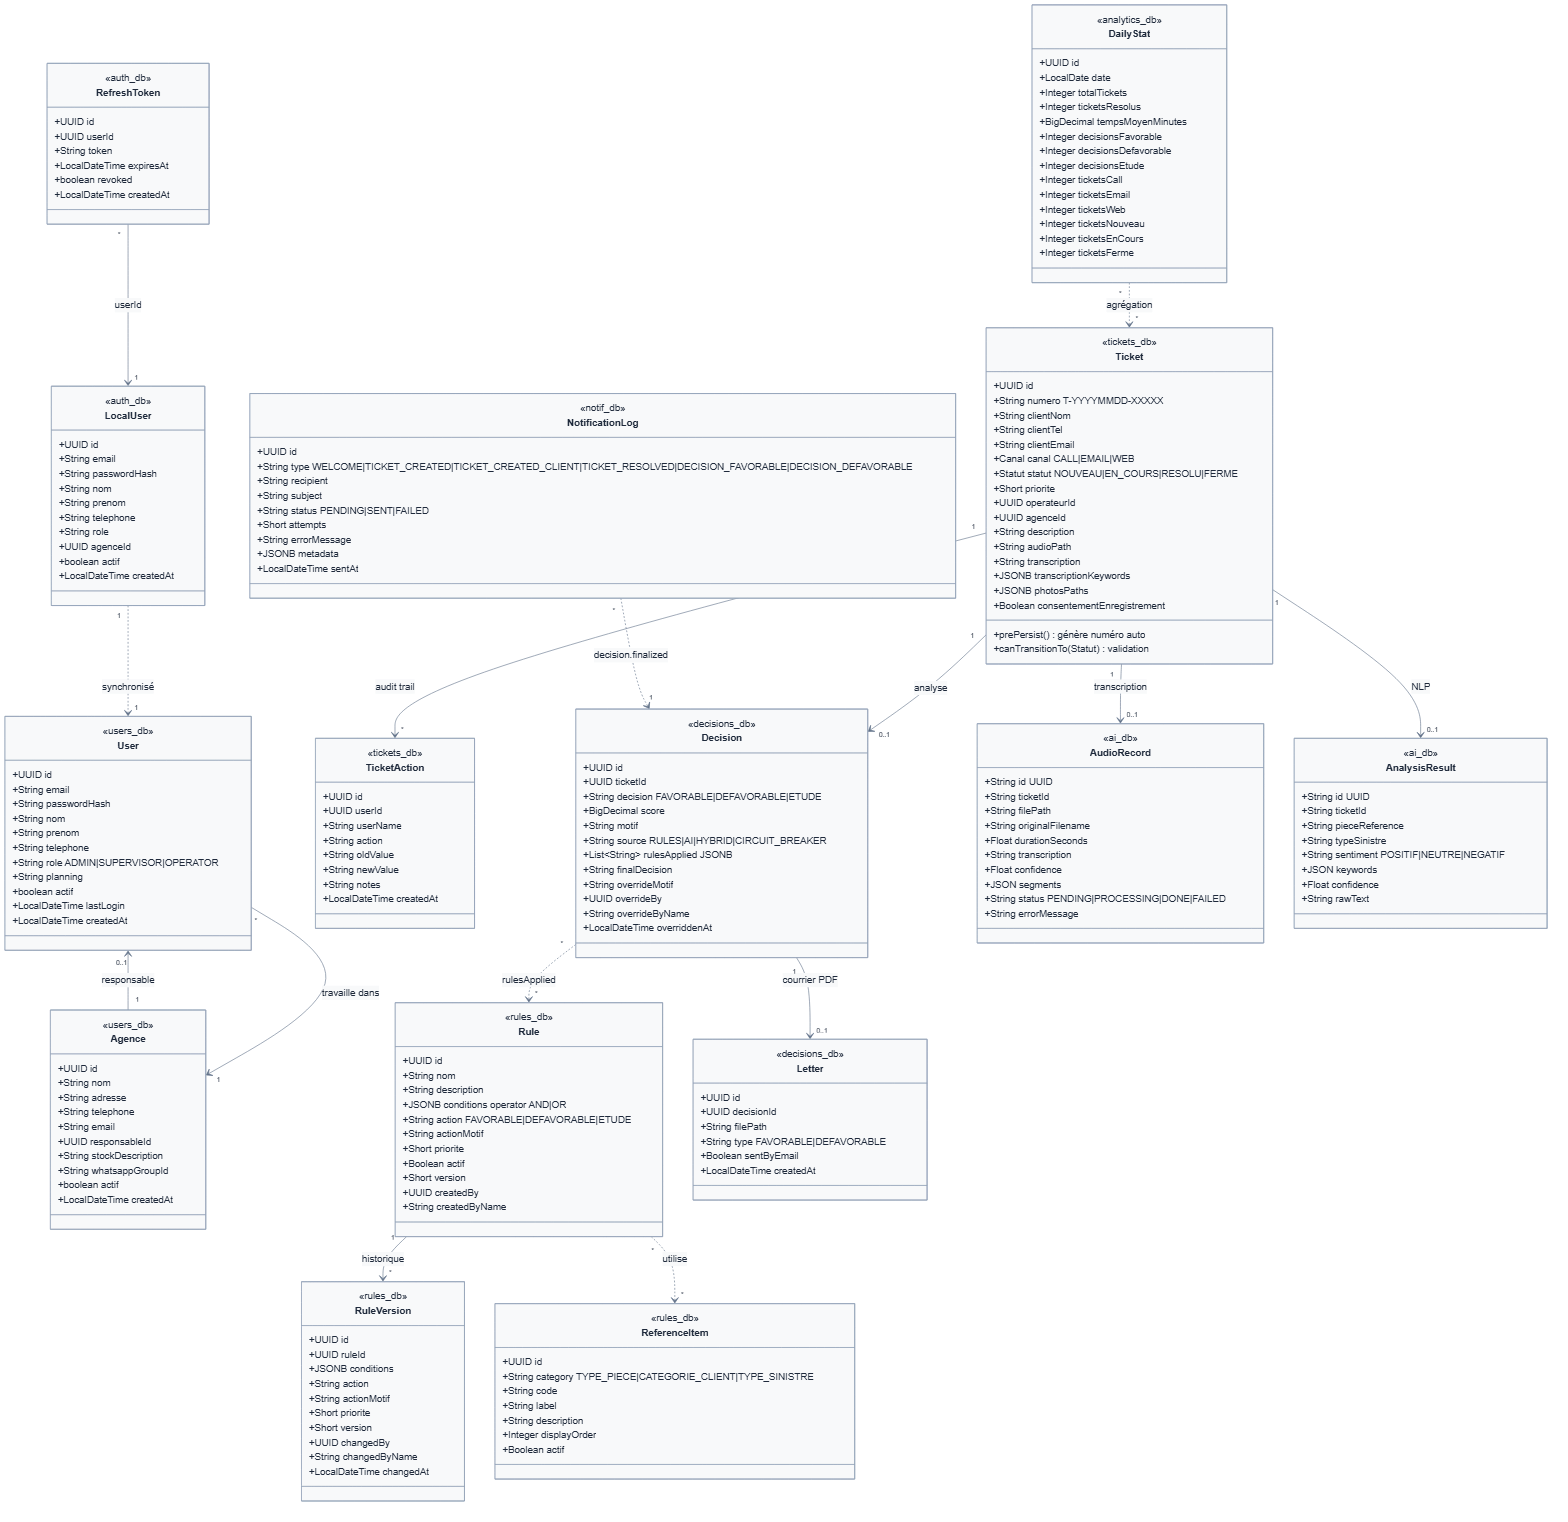
\includegraphics[width=\textwidth]{figures_uml_finaux/03_diagramme_de_classes_toutes_les_entits_15_entits_8_bases.png}
    \caption{Diagramme de classes global -- 15 entit\'{e}s sur 8 bases de donn\'{e}es}
    \label{fig:class_global}
\end{figure}

Nous d\'{e}taillons ci-dessous les diagrammes de classes des quatre services principaux.

\subsubsection{Diagramme de classes du auth-service}

\begin{figure}[htbp]
    \centering
    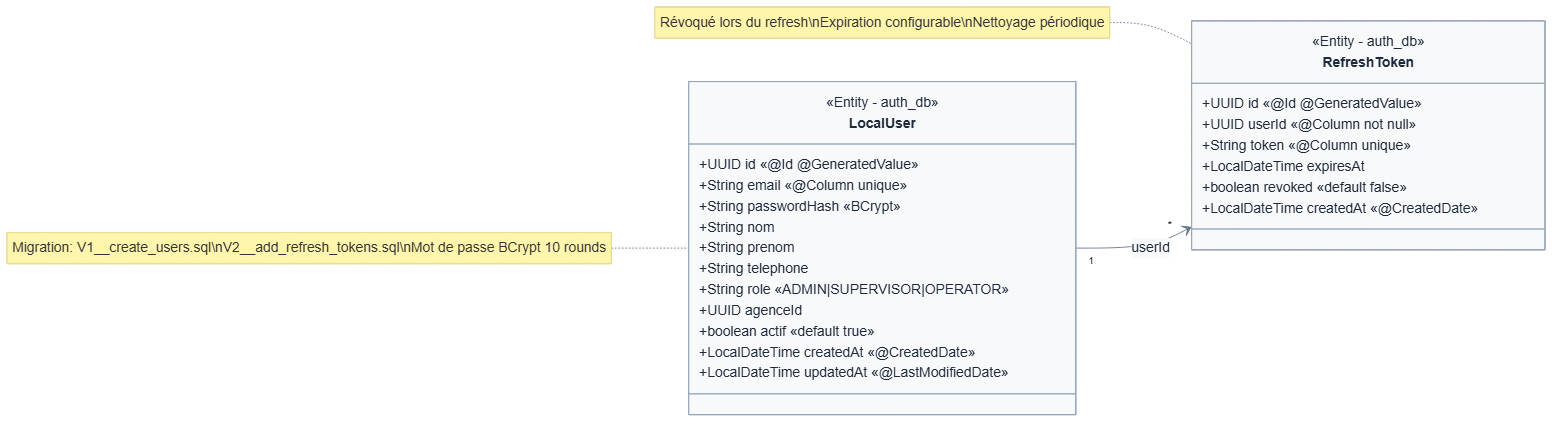
\includegraphics[width=0.85\textwidth]{figures_uml_finaux/38_diagramme_de_classes_entits_auth_db_auth-service.png}
    \caption{Diagramme de classes -- auth-service}
    \label{fig:class_auth}
\end{figure}

Le service d'authentification gère l'entité \texttt{LocalUser} avec les attributs~: id (UUID), email, passwordHash (BCrypt), nom, prenom, role (ADMIN/SUPERVISOR/OPERATOR), actif, agenceId. Il produit des tokens JWT (access 15min, refresh 7j) via la classe \texttt{JwtUtils}. L'entité \texttt{RefreshToken} stocke les jetons de rafraîchissement avec révocation.

\subsubsection{Diagramme de classes du ticket-service}

\begin{figure}[htbp]
    \centering
    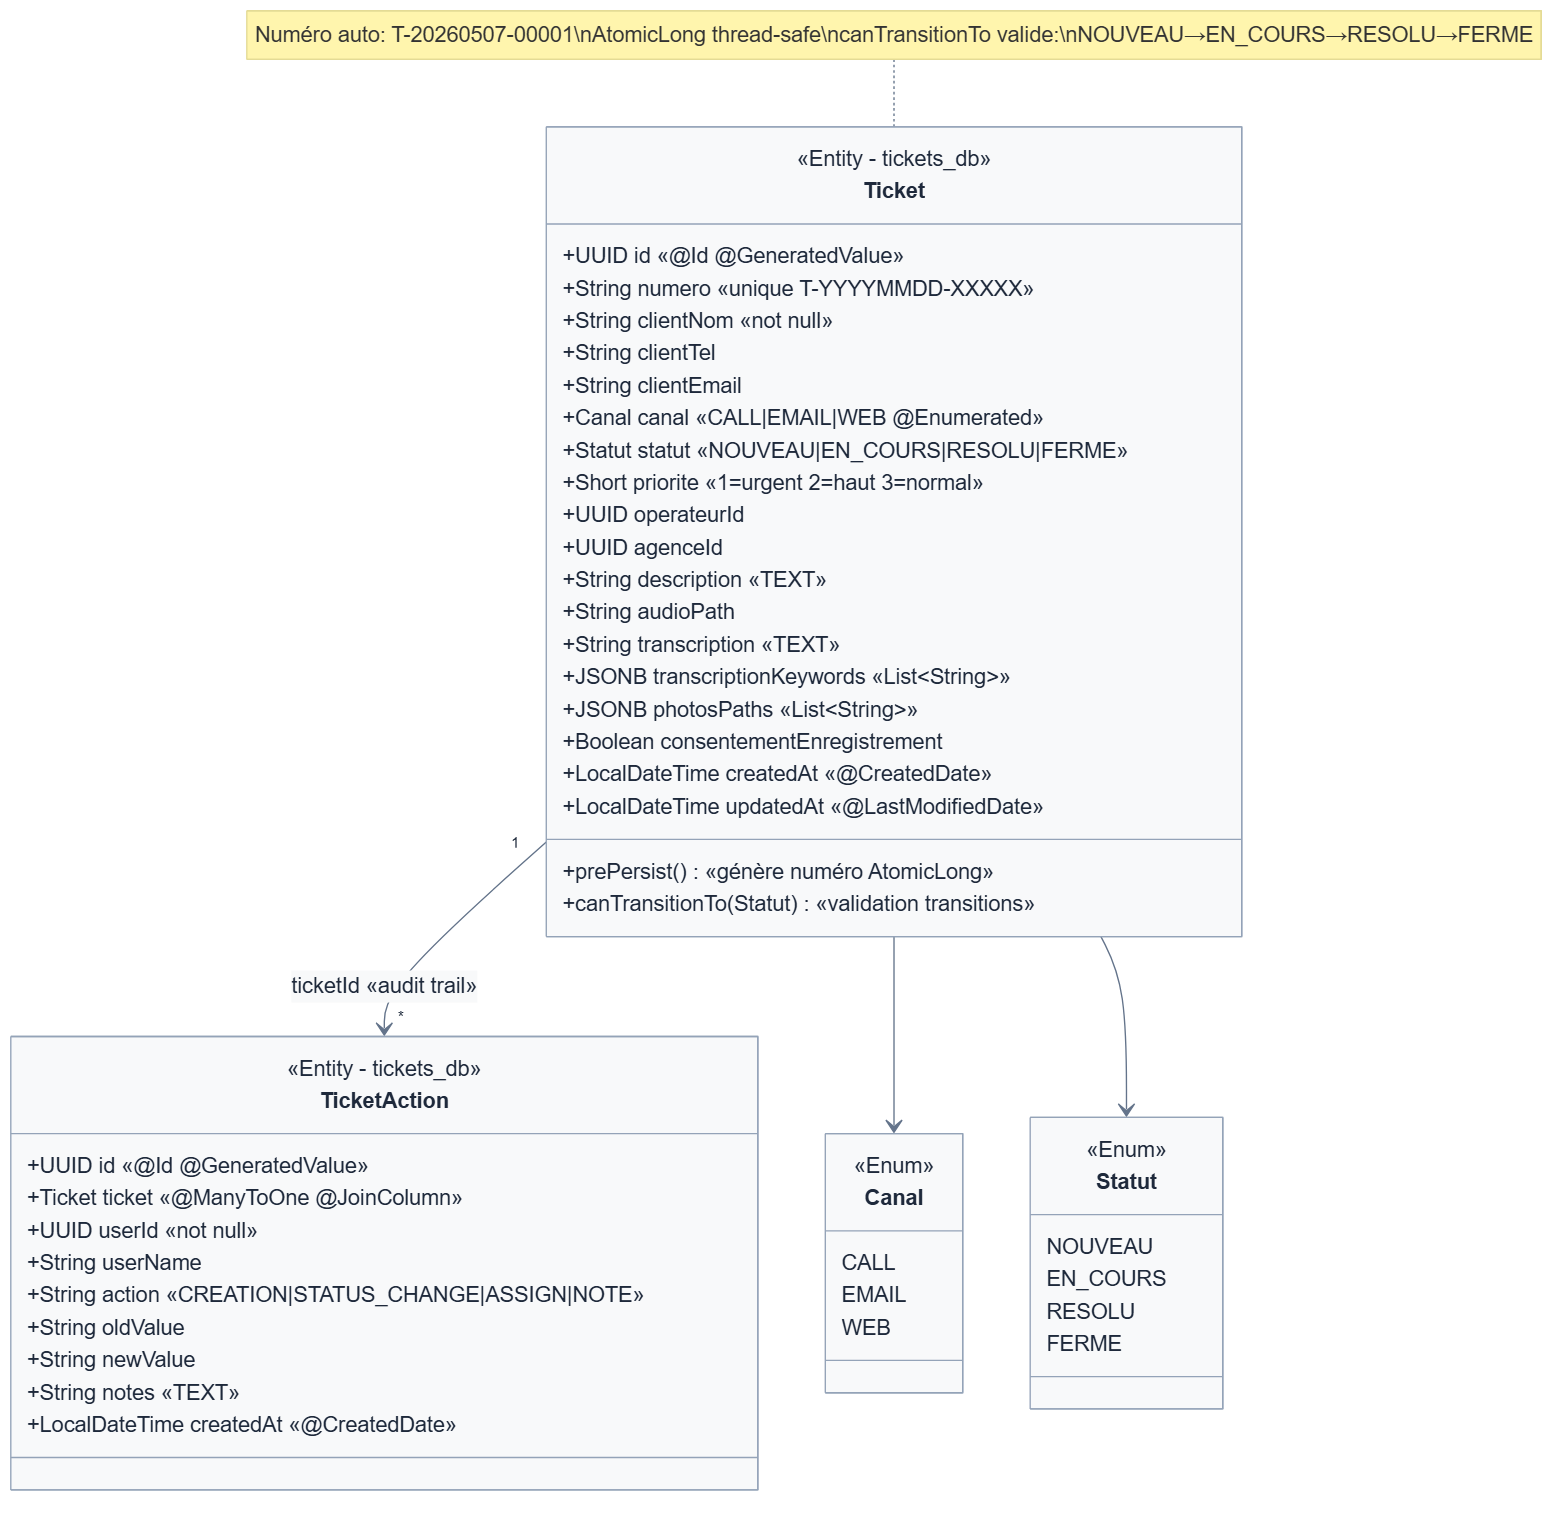
\includegraphics[width=0.85\textwidth]{figures_uml_finaux/40_diagramme_de_classes_entits_tickets_db_ticket-service.png}
    \caption{Diagramme de classes -- ticket-service}
    \label{fig:class_ticket}
\end{figure}

L'entité \texttt{Ticket} comprend~: id (UUID), numero (T-YYYYMMDD-XXXXX), canal (CALL/EMAIL/WEB), statut (NOUVEAU/EN\_COURS/RESOLU/FERME), priorite, clientNom, clientEmail, description, agenceId, operateurId, audioPath, transcription, transcriptionKeywords (JSONB), photosPaths (JSONB), consentementEnregistrement, timestamps. Le service gère également les \texttt{TicketAction} pour l'audit trail.

\subsubsection{Diagramme de classes du rules-service}

\begin{figure}[htbp]
    \centering
    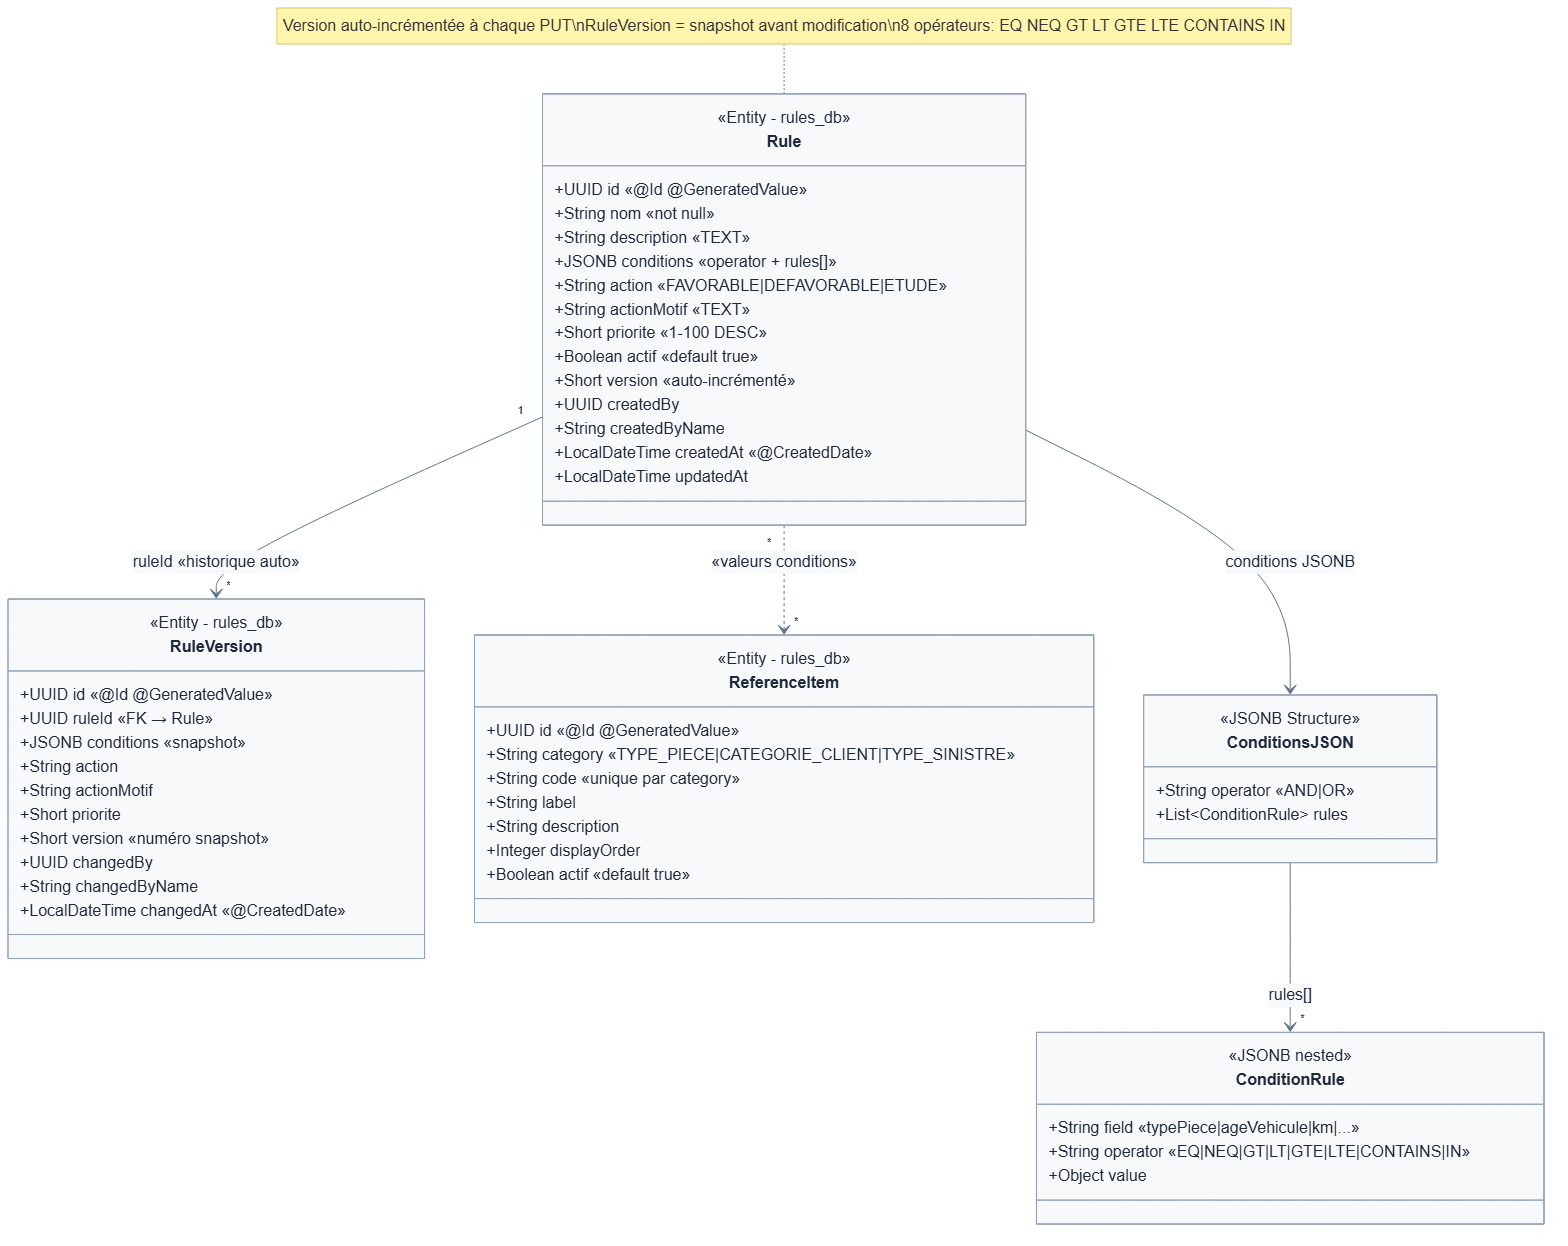
\includegraphics[width=0.85\textwidth]{figures_uml_finaux/41_diagramme_de_classes_entits_rules_db_rules-service.png}
    \caption{Diagramme de classes -- rules-service}
    \label{fig:class_rules}
\end{figure}

L'entité \texttt{Rule} contient~: id, nom, description, conditions (JSONB), action (FAVORABLE/DEFAVORABLE/ETUDE), actionMotif, priorite (1-10), actif, version, createdBy, createdByName, timestamps. Les conditions JSONB suivent le format~: \texttt{\{operator: "AND", conditions: [\{field, op, value\}]\}}. Le \texttt{RuleVersion} assure le versioning et le \texttt{ReferenceItem} gère le référentiel (types pièces, catégories clients, types sinistres).

\subsubsection{Diagramme de classes du decision-service}

\begin{figure}[htbp]
    \centering
    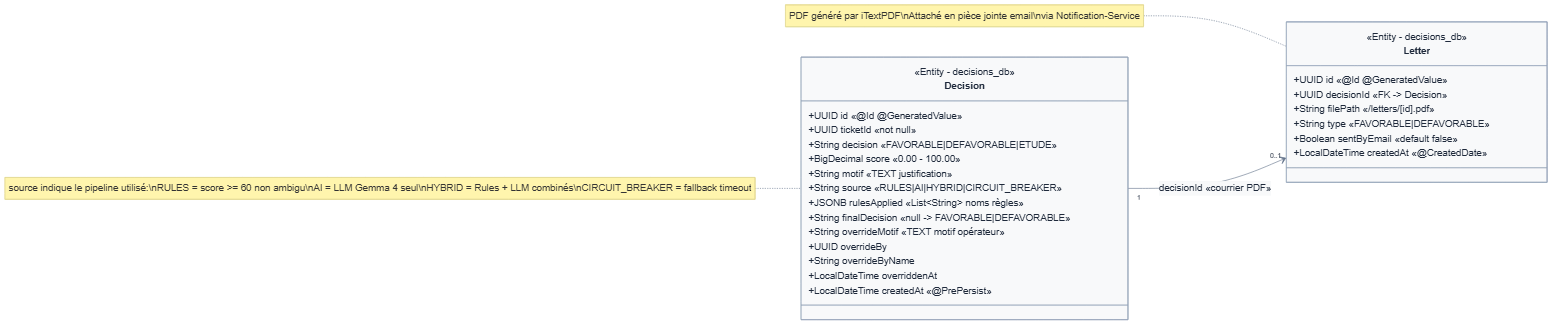
\includegraphics[width=0.85\textwidth]{figures_uml_finaux/42_diagramme_de_classes_entits_decisions_db_decision-service.png}
    \caption{Diagramme de classes -- decision-service}
    \label{fig:class_decision}
\end{figure}

L'entité \texttt{Decision} comprend~: id, ticketId, decision (FAVORABLE/DEFAVORABLE/ETUDE), score (BigDecimal), motif, source (RULES/AI/HYBRID/CIRCUIT\_BREAKER), rulesApplied (JSONB), finalDecision, overrideMotif, overrideBy, overrideByName, overriddenAt. L'entité \texttt{Letter} stocke les courriers PDF générés (relation 1:0..1 avec Decision). Le service utilise \texttt{StringRedisTemplate} pour le cache et \texttt{RabbitTemplate} pour publier les événements.

\subsection{Vue Dynamique~: diagrammes de s\'{e}quence}

La vue dynamique d\'{e}crit le comportement du syst\`{e}me, c'est-\`{a}-dire la fa\c{c}on dont les objets interagissent et \'{e}voluent au fil du temps. Elle est principalement illustr\'{e}e par le diagramme de s\'{e}quence, qui met en \'{e}vidence les \'{e}changes entre les diff\'{e}rents composants du syst\`{e}me. Dans notre architecture microservices, chaque diagramme fait intervenir plusieurs services communiquant via REST ou RabbitMQ.

\subsubsection{Diagramme de s\'{e}quence \og~Authentification~\fg{}}

\begin{figure}[htbp]
    \centering
    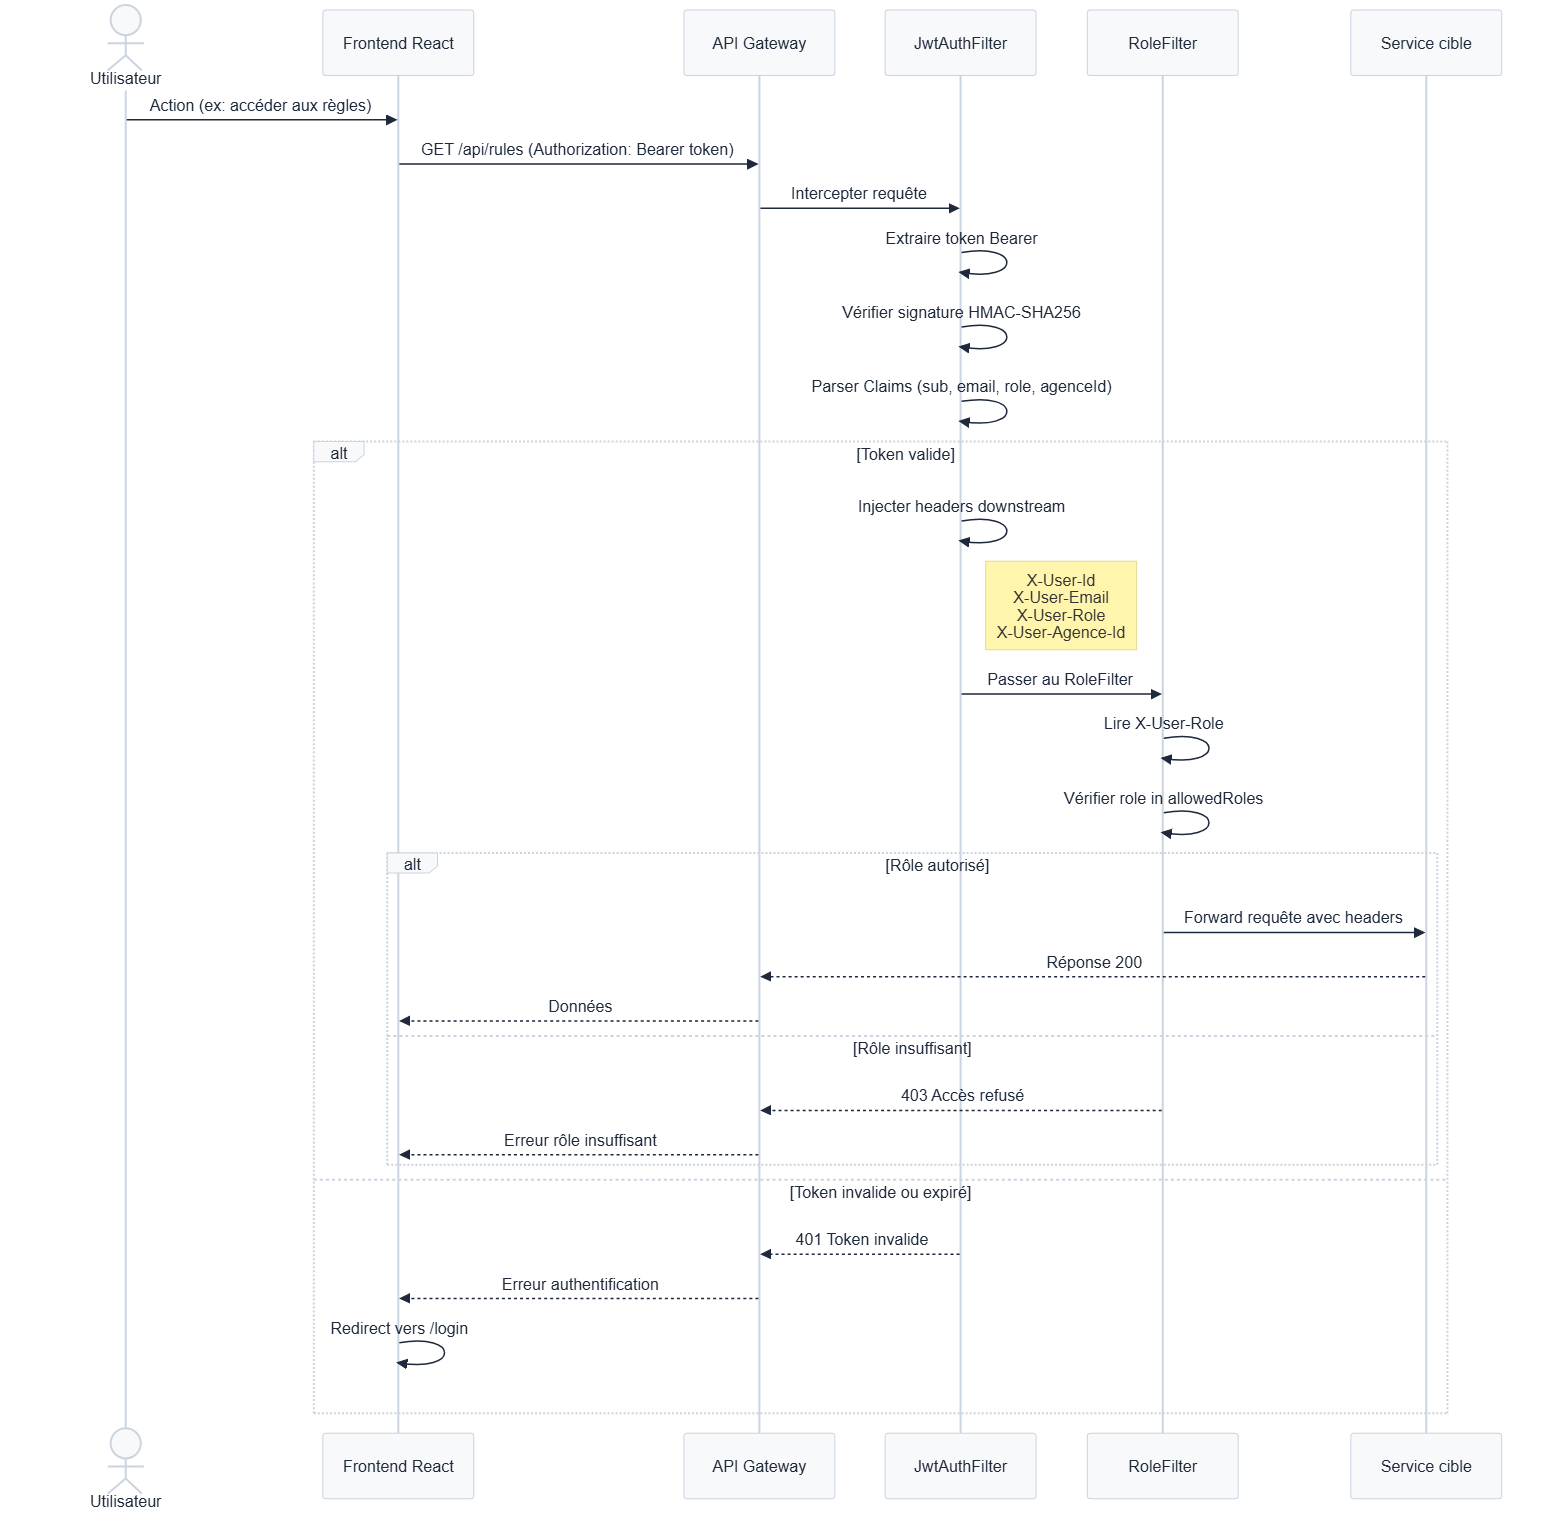
\includegraphics[width=0.90\textwidth]{figures_uml_finaux/12_diagramme_de_squence_scurit_jwt_rbac_gateway.png}
    \caption{Diagramme de séquence -- Authentification JWT}
    \label{fig:seq_auth}
\end{figure}

Ce diagramme illustre le flux d'authentification JWT. L'utilisateur envoie ses identifiants au gateway, qui les transmet au auth-service. Apr\`{e}s v\'{e}rification BCrypt, un token d'acc\`{e}s (15 min) et un token de rafra\^{i}chissement (7 jours) sont g\'{e}n\'{e}r\'{e}s. Les requ\^{e}tes suivantes sont valid\'{e}es par le gateway via le filtre RBAC.

\subsubsection{Diagramme de s\'{e}quence \og~Cr\'{e}er un ticket multicanal~\fg{}}

\begin{figure}[htbp]
    \centering
    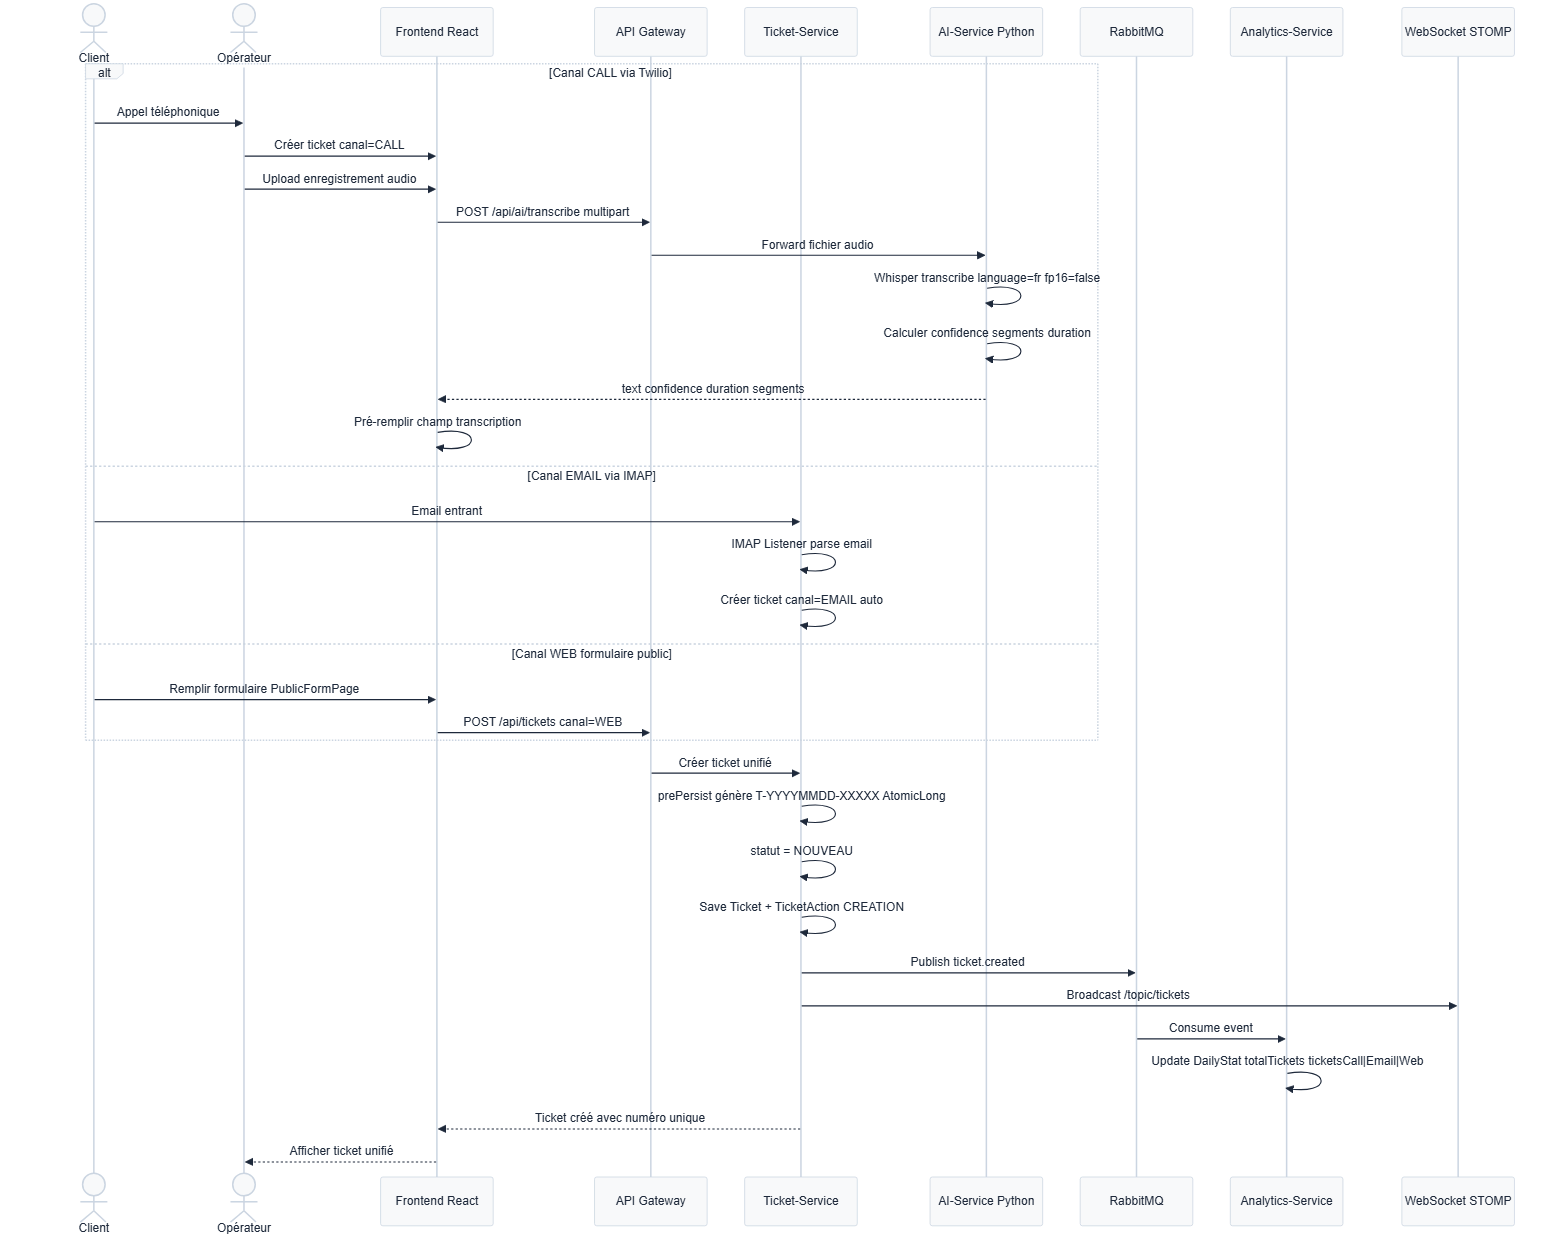
\includegraphics[width=0.90\textwidth]{figures_uml_finaux/05_diagramme_de_squence_cration_ticket_multicanal_centralis.png}
    \caption{Diagramme de séquence -- Création de ticket multicanal}
    \label{fig:seq_ticket}
\end{figure}

Ce diagramme montre la cr\'{e}ation d'un ticket \`{a} partir des trois canaux (appel Twilio, email IMAP, formulaire web). Le ticket-service centralise les demandes, g\'{e}n\`{e}re un num\'{e}ro unique (T-YYYYMMDD-XXXXX), puis publie l'\'{e}v\'{e}nement \texttt{ticket.created} sur RabbitMQ pour d\'{e}clencher les traitements asynchrones.

\subsubsection{Diagramme d'activit\'{e} \og~Transcription audio et analyse NLP~\fg{}}

\begin{figure}[htbp]
    \centering
    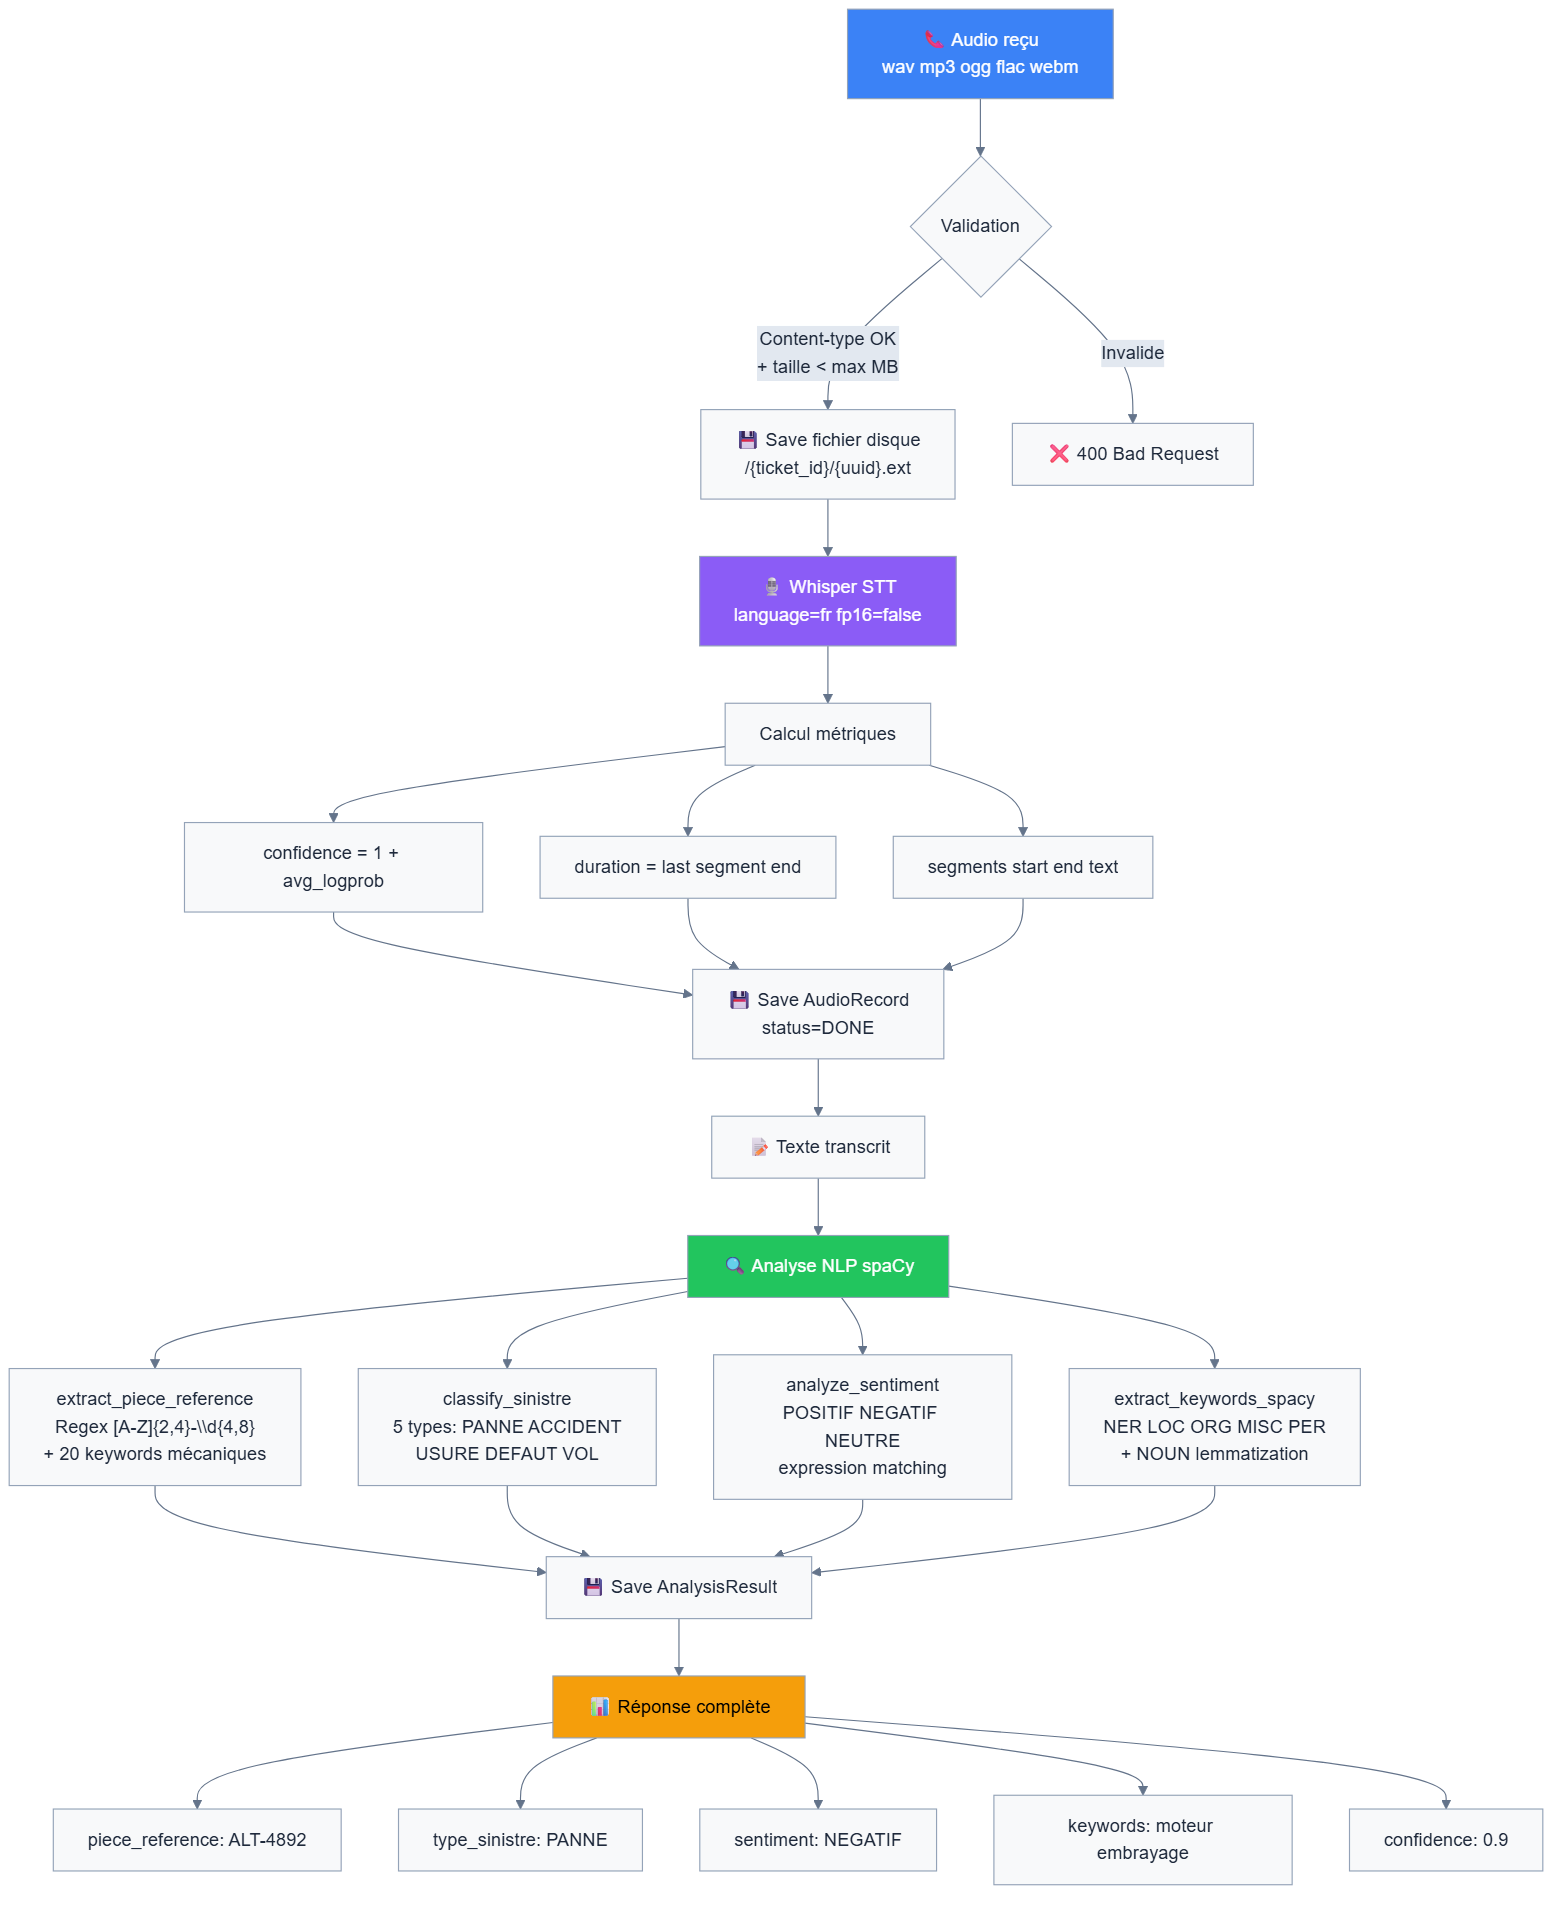
\includegraphics[width=0.90\textwidth]{figures_uml_finaux/20_diagramme_dactivit_pipeline_nlp_complet_whisper_spacy.png}
    \caption{Diagramme d'activit\'{e} -- Transcription audio et analyse NLP}
    \label{fig:seq_transcription}
\end{figure}

Ce diagramme d\'{e}taille le pipeline NLP complet~: l'audio est envoy\'{e} au ai-service qui utilise Whisper pour la transcription, puis spaCy pour l'extraction des mots-cl\'{e}s, la d\'{e}tection du type de sinistre et l'analyse de sentiment. Les r\'{e}sultats sont retourn\'{e}s au ticket-service pour pr\'{e}-remplir le formulaire.

\subsubsection{Diagramme de s\'{e}quence \og~Analyse d\'{e}cisionnelle (pipeline 3 \'{e}tapes)~\fg{}}

\begin{figure}[htbp]
    \centering
    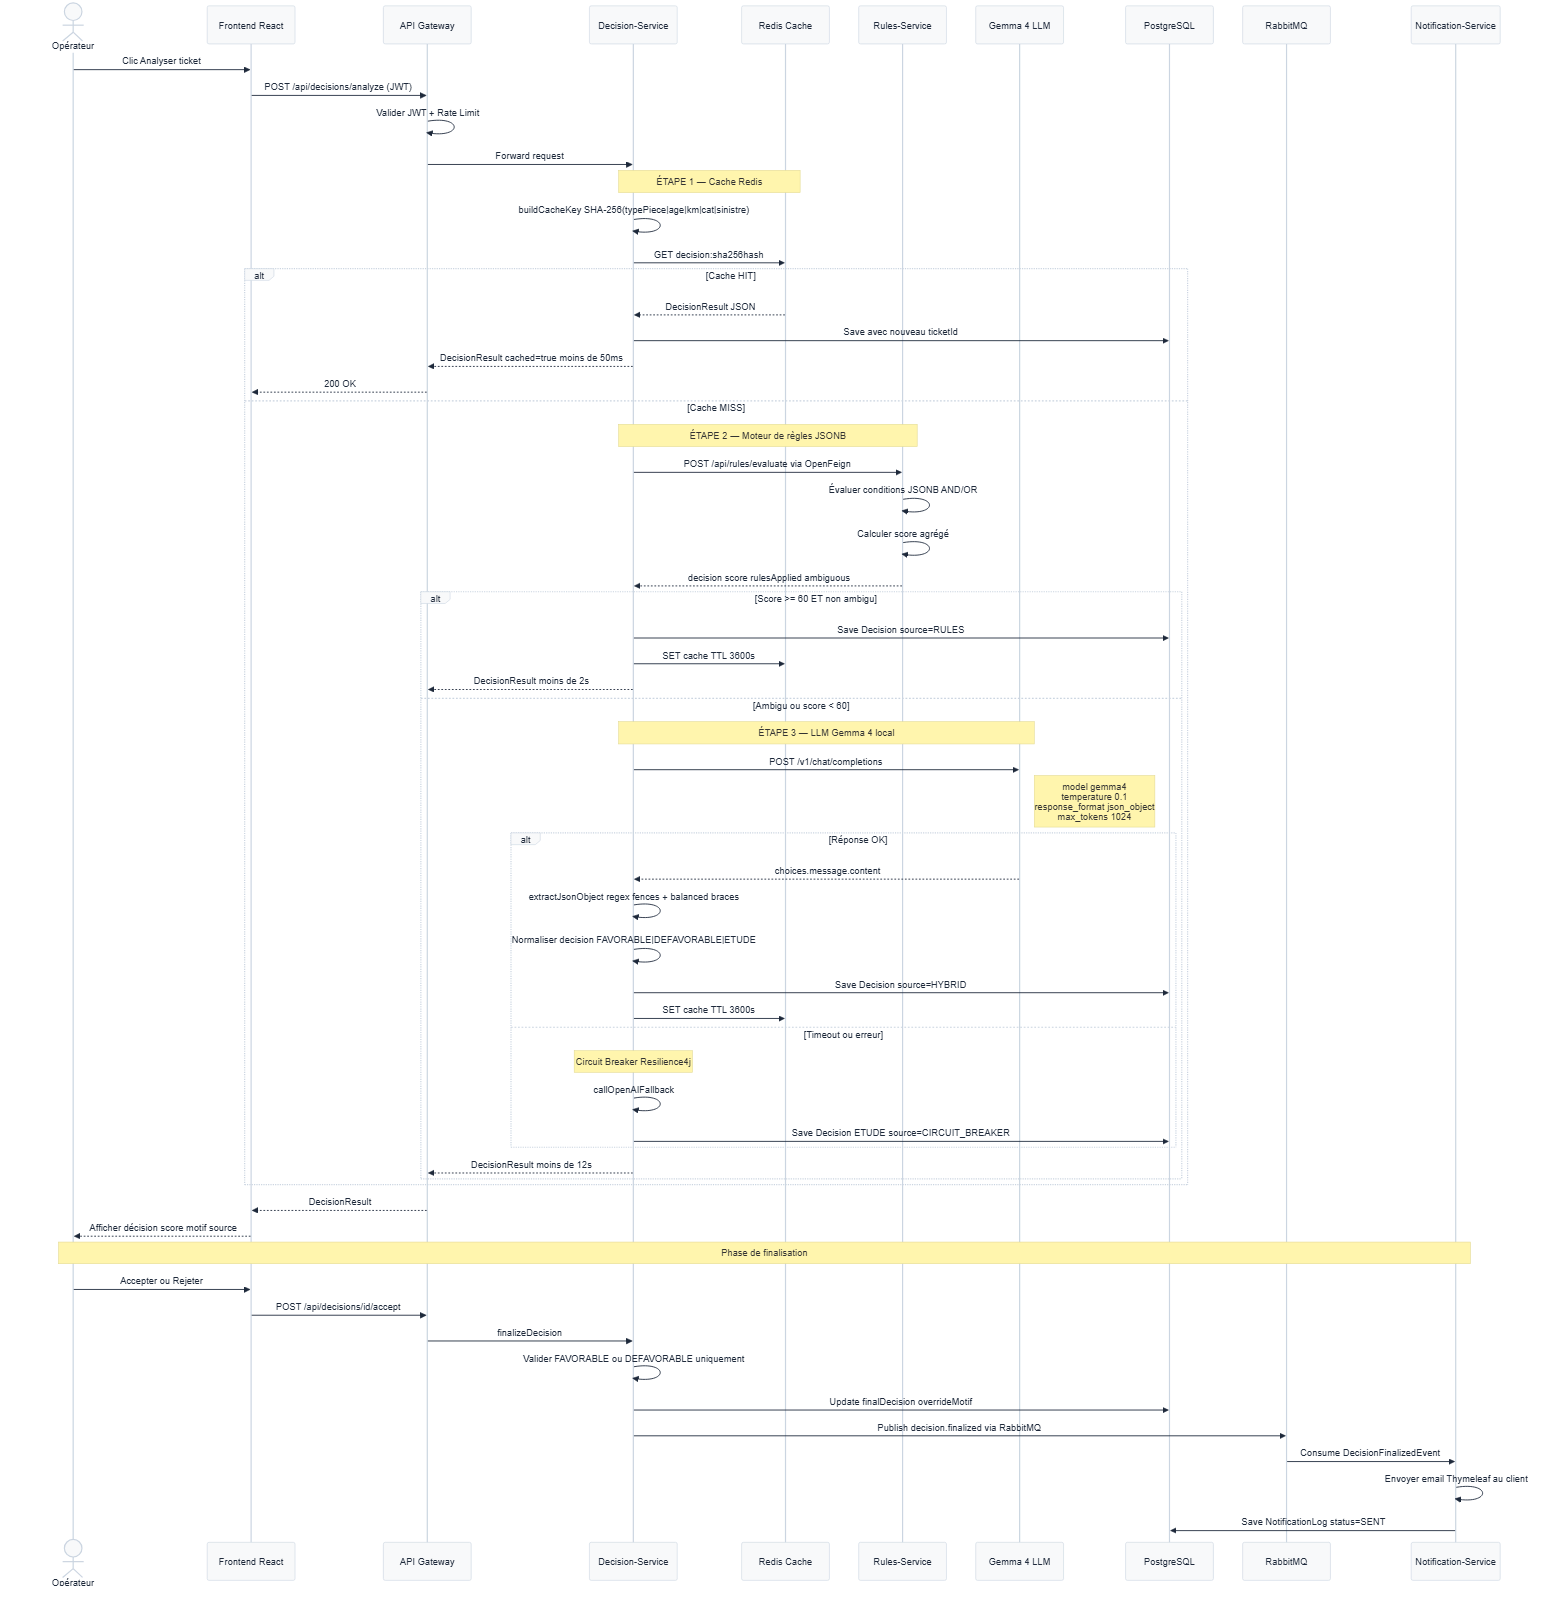
\includegraphics[width=0.95\textwidth]{figures_uml_finaux/04_diagramme_de_squence_pipeline_dcisionnel_3_tapes.png}
    \caption{Diagramme de séquence -- Pipeline de décision en 3 étapes}
    \label{fig:seq_decision}
\end{figure}

Ce diagramme pr\'{e}sente le flux du pipeline d\'{e}cisionnel en trois \'{e}tapes successives (cache Redis, moteur de r\`{e}gles, LLM). Chaque \'{e}tape est tent\'{e}e s\'{e}quentiellement~: si le cache retourne un r\'{e}sultat, les \'{e}tapes suivantes sont ignor\'{e}es. La d\'{e}cision finale est stock\'{e}e en base et publi\'{e}e via RabbitMQ.

\subsubsection{Diagramme de s\'{e}quence \og~Chatbot WhatsApp RAG~\fg{}}

\begin{figure}[htbp]
    \centering
    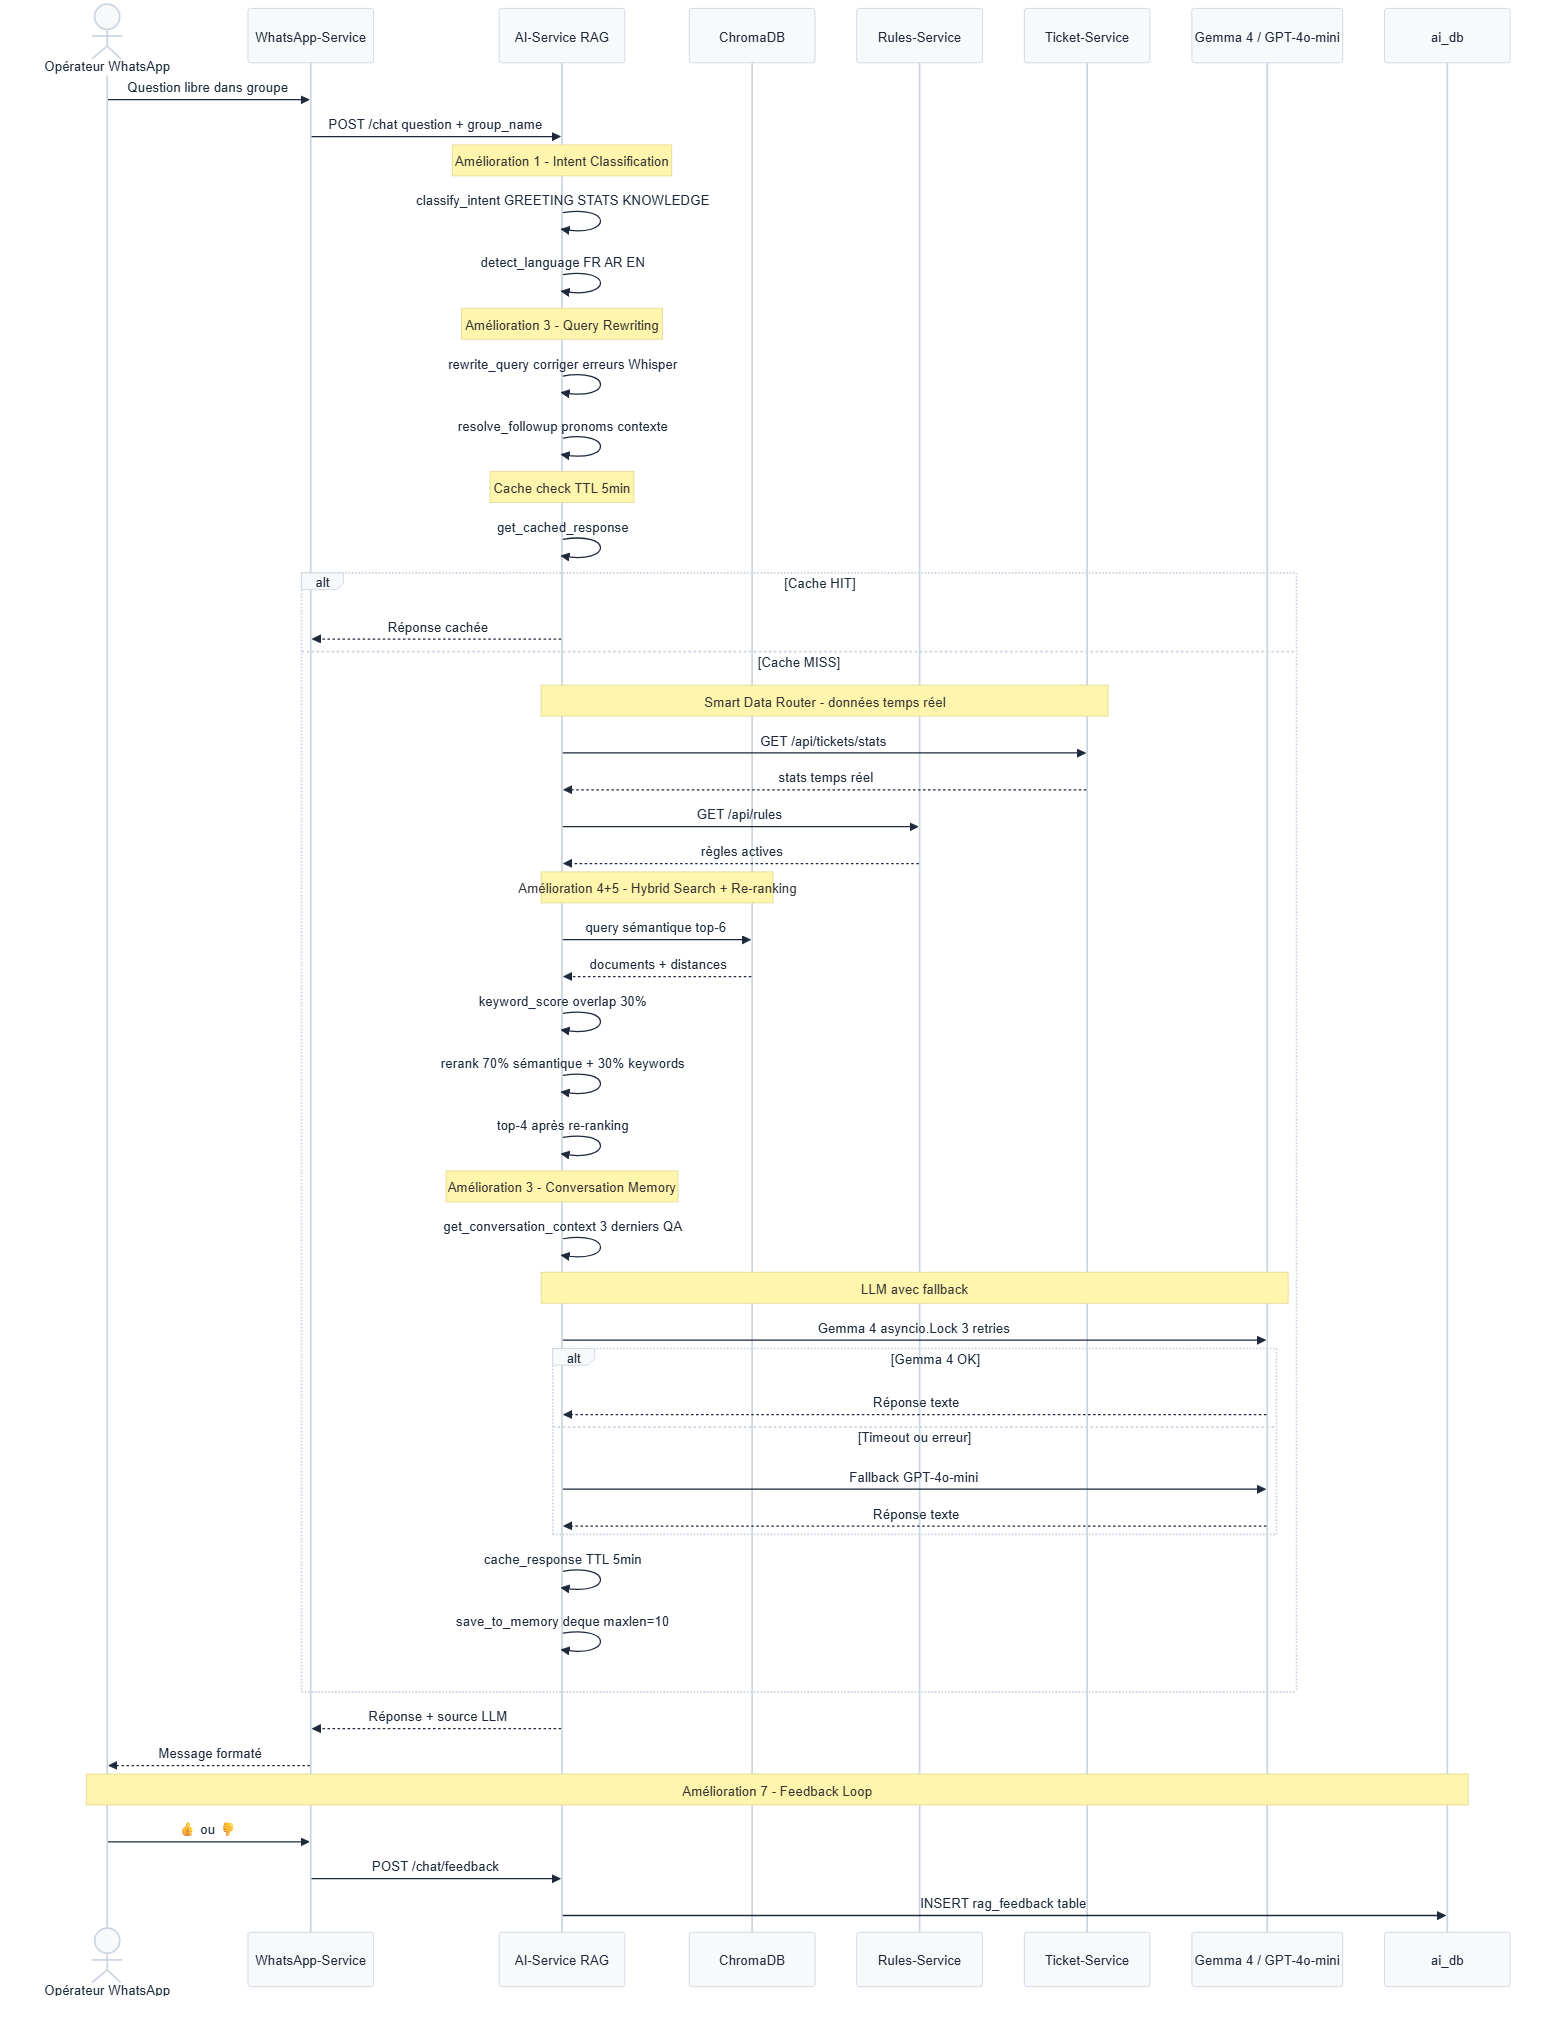
\includegraphics[width=0.95\textwidth]{figures_uml_finaux/19_diagramme_de_squence_pipeline_rag_chatbot_8_amliorations_ia.png}
    \caption{Diagramme de séquence -- Interrogation du chatbot WhatsApp}
    \label{fig:seq_chatbot}
\end{figure}

Ce diagramme illustre le flux RAG du chatbot~: le message WhatsApp est re\c{c}u par le whatsapp-service, transmis au ai-service qui effectue une recherche hybride (s\'{e}mantique + mots-cl\'{e}s) dans ChromaDB, puis g\'{e}n\`{e}re une r\'{e}ponse contextuelle via le LLM.

\subsubsection{Diagramme de s\'{e}quence \og~Configurer une r\`{e}gle d'assurance~\fg{}}

\begin{figure}[htbp]
    \centering
    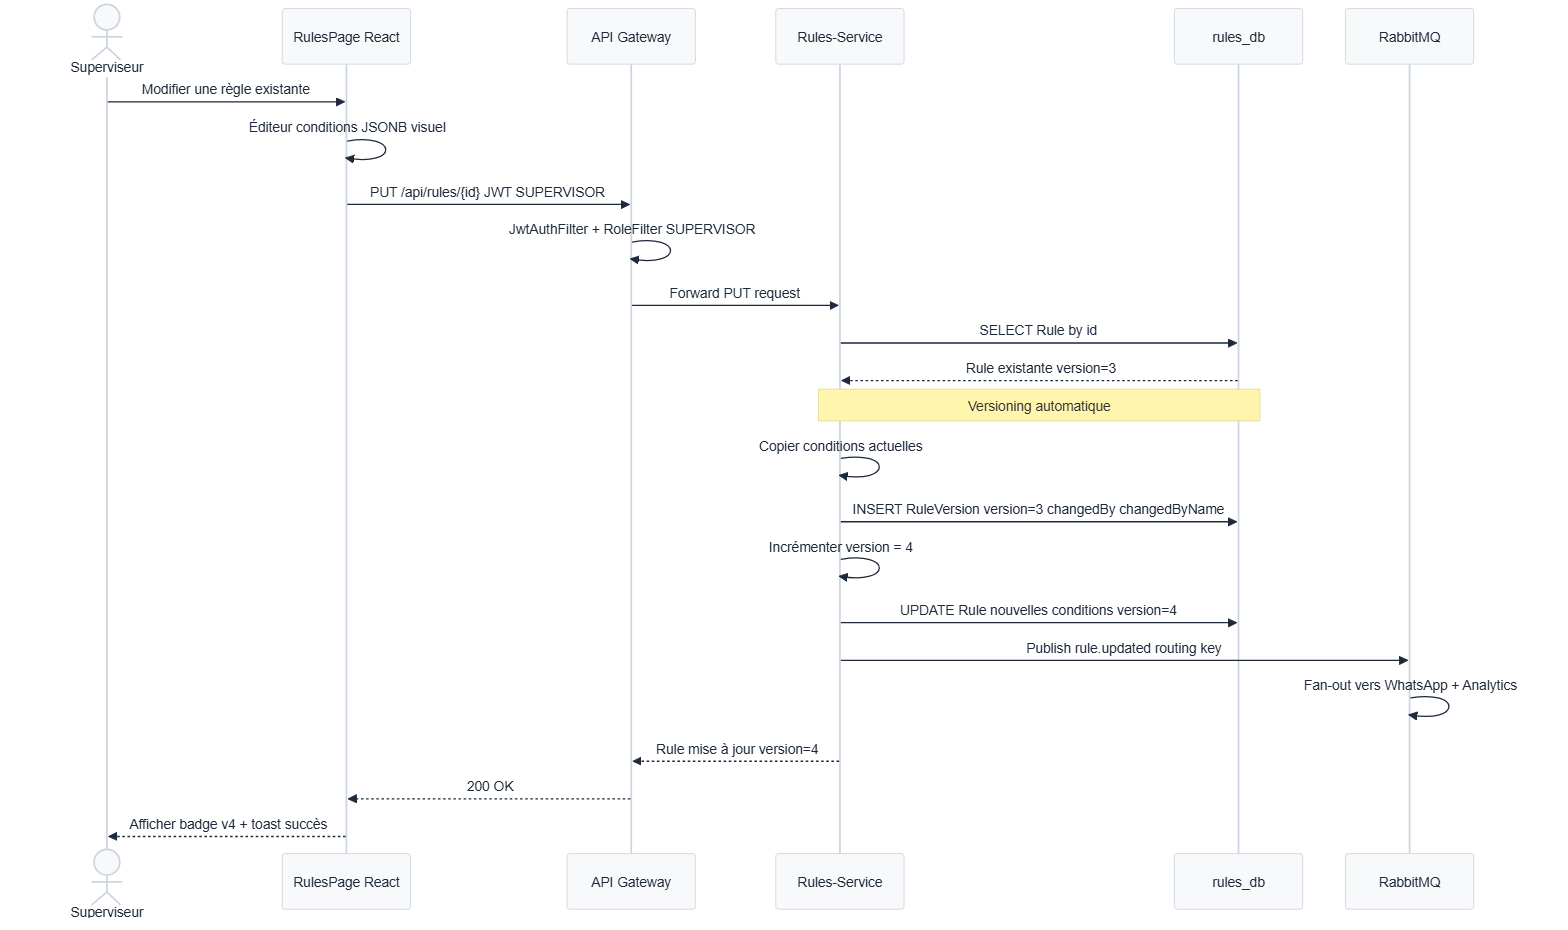
\includegraphics[width=0.90\textwidth]{figures_uml_finaux/26_diagramme_de_squence_rule_crud_versioning_automatique.png}
    \caption{Diagramme de séquence -- Configuration d'une règle d'assurance}
    \label{fig:seq_rules}
\end{figure}

Ce diagramme montre le flux CRUD d'une r\`{e}gle d'assurance avec versioning automatique. Lorsqu'un superviseur modifie une r\`{e}gle, l'ancienne version est archiv\'{e}e dans \texttt{rule\_versions} et la nouvelle version est enregistr\'{e}e avec un num\'{e}ro incr\'{e}ment\'{e}.

\subsubsection{Diagramme de s\'{e}quence \og~Notification et envoi de courrier~\fg{}}

\begin{figure}[htbp]
    \centering
    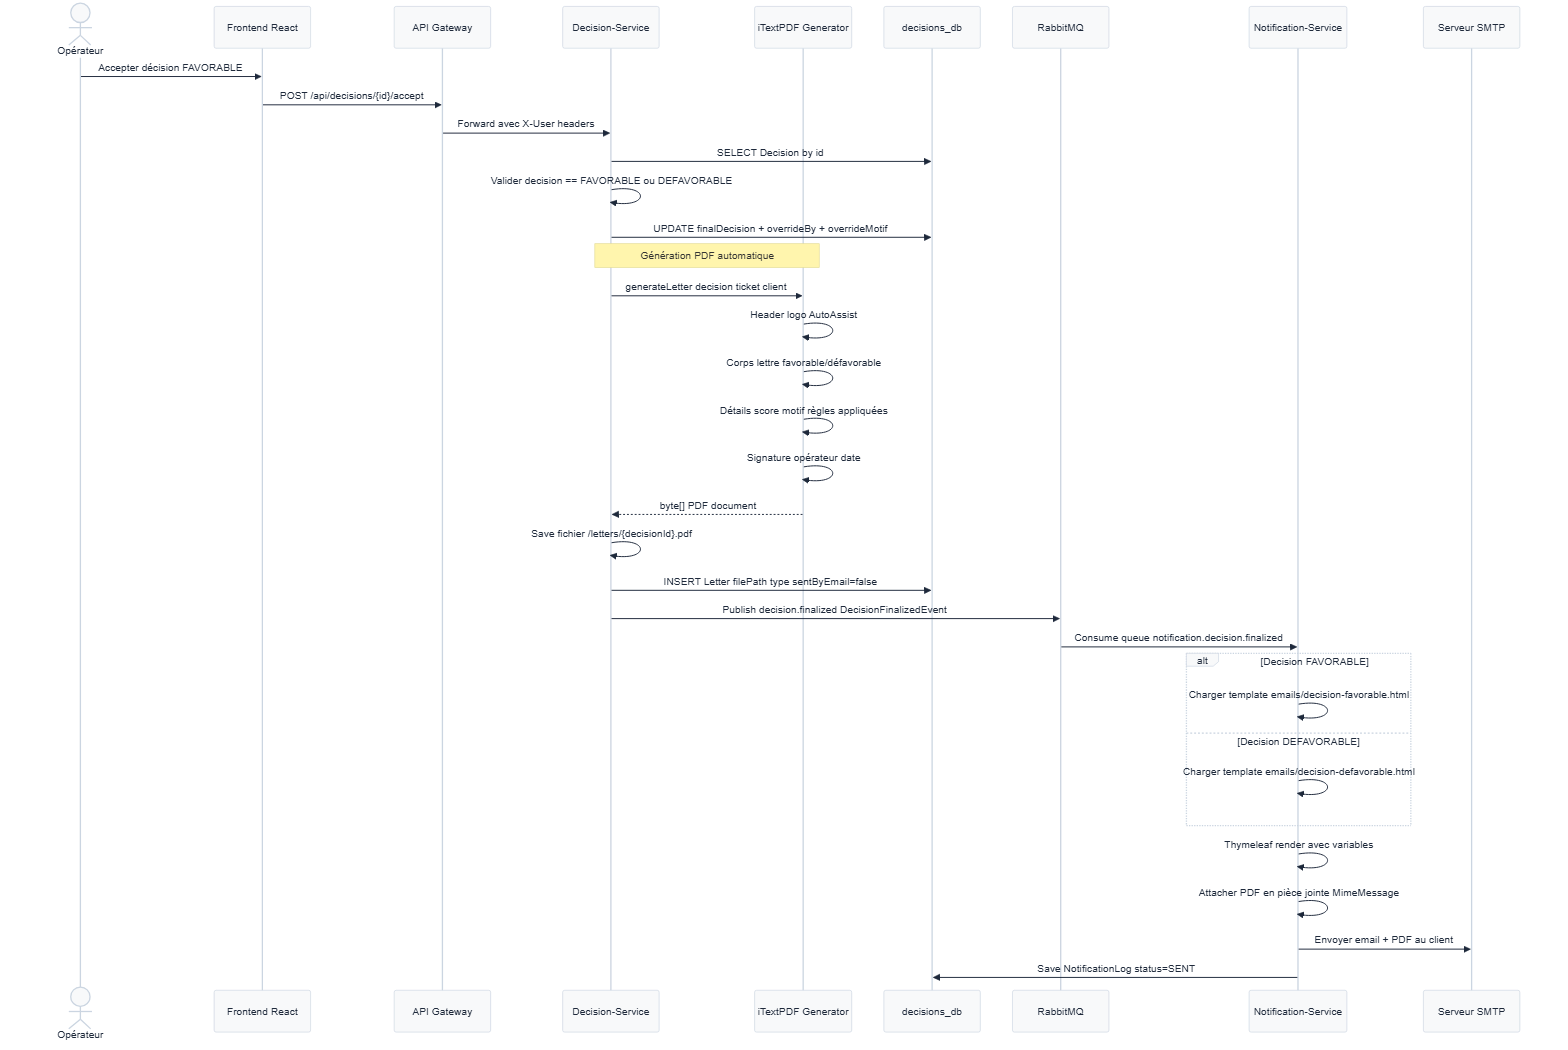
\includegraphics[width=0.90\textwidth]{figures_uml_finaux/30_diagramme_de_squence_gnration_courrier_pdf_letter.png}
    \caption{Diagramme de séquence -- Notification et envoi de courrier PDF}
    \label{fig:seq_notification}
\end{figure}

Ce diagramme d\'{e}taille le flux de notification~: apr\`{e}s la finalisation d'une d\'{e}cision, le notification-service g\'{e}n\`{e}re un courrier PDF via un template Thymeleaf, l'envoie par email avec pi\`{e}ce jointe, et enregistre la notification dans \texttt{notification\_logs}.

\subsection{Conception de la base de donn\'{e}es}

Le syst\`{e}me utilise une approche \textbf{Database-per-Service}, chaque microservice poss\'{e}dant sa propre base PostgreSQL.

\begin{sidewaysfigure}
    \centering
    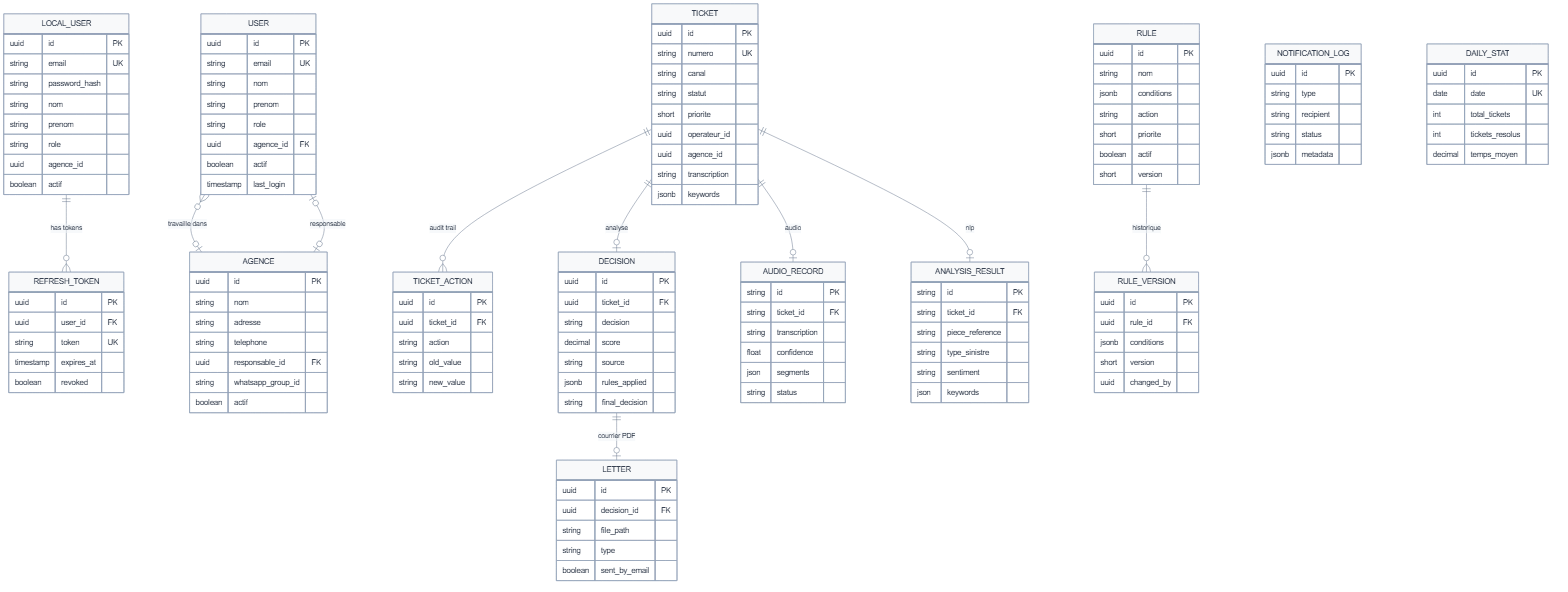
\includegraphics[width=\textheight]{figures_uml_finaux/29_diagramme_er_schma_base_de_donnes_9_dbs.png}
    \caption{Schéma global de la base de données (Database-per-Service)}
    \label{fig:bdd}
\end{sidewaysfigure}

\begin{table}[H]
\centering
\caption{Bases de données par microservice}
\label{tab:bdd}
\begin{tabular}{|p{3cm}|p{2.5cm}|p{7.5cm}|}
\hline
\textbf{Service} & \textbf{Base} & \textbf{Tables principales} \\
\hline
auth-service & auth\_db & local\_users, refresh\_tokens \\
\hline
organisation-service & users\_db & users, agences \\
\hline
ticket-service & tickets\_db & tickets, ticket\_actions \\
\hline
rules-service & rules\_db & rules, rule\_versions, reference\_items \\
\hline
decision-service & decisions\_db & decisions, letters \\
\hline
notification-service & notif\_db & notification\_logs \\
\hline
analytics-service & analytics\_db & daily\_stats \\
\hline
ai-service & ai\_db & audio\_records, analysis\_results \\
\hline
\end{tabular}
\end{table}


\subsection{Pile technologique}

Le syst\`{e}me AutoAssist repose sur une architecture polyglotte adapt\'{e}e aux besoins de chaque couche. Le tableau~\ref{tab:techstack} pr\'{e}sente les technologies utilis\'{e}es et leur justification.

\begin{table}[H]
\centering
\caption{Pile technologique du syst\`{e}me AutoAssist}
\label{tab:techstack}
\small
\begin{tabular}{|p{2.5cm}|p{3cm}|p{7cm}|}
\hline
\textbf{Composant} & \textbf{Technologie} & \textbf{Justification} \\
\hline
Services m\'{e}tier (x7) & Java 21 / Spring Boot 3 & Robustesse, \'{e}cosyst\`{e}me Spring Cloud (Eureka, Feign, Gateway), typage statique \\
\hline
Service IA & Python FastAPI & Support natif de l'asynchrone, int\'{e}gration Whisper/spaCy/PyTorch, performance HTTP \\
\hline
Service WhatsApp & Node.js & Biblioth\`{e}que \texttt{whatsapp-web.js}, traitement \'{e}v\'{e}nementiel asynchrone \\
\hline
Frontend Web & React 18 / Vite & Flexibilit\'{e} pour le tableau de bord d'administration, composants r\'{e}utilisables \\
\hline
Application Mobile & Flutter & D\'{e}veloppement cross-platform pour les op\'{e}rateurs nomades \\
\hline
Base de donn\'{e}es & PostgreSQL 15 & Transactions ACID, support JSONB pour les conditions des r\`{e}gles m\'{e}tier \\
\hline
Base vectorielle & ChromaDB & Stockage des embeddings pour la recherche s\'{e}mantique RAG \\
\hline
Transcription audio & OpenAI Whisper & Transcription pr\'{e}cise des appels clients en fran\c{c}ais et arabe \\
\hline
Analyse NLP & spaCy & Extraction d'entit\'{e}s et analyse de sentiment rapide et efficace \\
\hline
LLM & Gemma~4 (local) & Mod\`{e}le open-source ex\'{e}cut\'{e} via Docker Model Runner, confidentialit\'{e} des donn\'{e}es \\
\hline
Cache & Redis 7 & Stockage TTL des d\'{e}cisions calcul\'{e}es pour \'{e}viter les recalculs co\^{u}teux \\
\hline
Messagerie & RabbitMQ 3 & D\'{e}couplage asynchrone entre services, garantie de livraison des \'{e}v\'{e}nements \\
\hline
\end{tabular}
\end{table}

\subsection{Strat\'{e}gie de tests}

Pour garantir la qualit\'{e} du syst\`{e}me, une strat\'{e}gie de tests multi-niveaux est pr\'{e}vue~:

\begin{itemize}
    \item \textbf{Tests unitaires}~: chaque service Java est couvert par des tests JUnit~5 avec Mockito pour les mocks. Le service IA Python utilise pytest. L'objectif est une couverture sup\'{e}rieure \`{a} 75\%~;
    \item \textbf{Tests d'int\'{e}gration}~: v\'{e}rification des appels inter-services (Feign), de la communication RabbitMQ et des acc\`{e}s base de donn\'{e}es~;
    \item \textbf{Tests de contr\^{o}leurs}~: validation des endpoints REST avec MockMvc (codes HTTP, corps de r\'{e}ponse, gestion des erreurs)~;
    \item \textbf{Int\'{e}gration continue}~: GitHub Actions ex\'{e}cute automatiquement tous les tests \`{a} chaque push, bloquant le merge en cas d'\'{e}chec.
\end{itemize}

\section*{Conclusion}
\label{sec:conclusion_ch2}

Dans ce chapitre, nous avons pr\'{e}sent\'{e} la conception technique du syst\`{e}me AutoAssist. L'architecture microservices, organis\'{e}e en cinq couches avec dix-sept conteneurs Docker, combine une communication synchrone (REST/OpenFeign) et asynchrone (RabbitMQ), renforc\'{e}e par des m\'{e}canismes de r\'{e}silience (cache Redis, Circuit Breaker). Les deux innovations majeures --- le pipeline d\'{e}cisionnel en trois \'{e}tapes et l'architecture RAG du chatbot --- ont \'{e}t\'{e} d\'{e}taill\'{e}es. La conception a \'{e}t\'{e} mod\'{e}lis\'{e}e via des diagrammes de classes et de s\'{e}quence. Le chapitre suivant sera consacr\'{e} \`{a} la r\'{e}alisation et aux r\'{e}sultats obtenus.

% --- Chapitres suivants masqués (soutenance mi-parcours) ---
% \chapter{R\'{e}alisation}
\label{chap:realisation}

\vspace{2cm}

\noindent\textbf{\Large Plan}

\vspace{0.5cm}
\noindent\rule{\textwidth}{0.4pt}
\vspace{0.3cm}

\begin{list}{}{\setlength{\leftmargin}{1.5cm}\setlength{\itemsep}{6pt}}
  \item \textbf{1} \hspace{0.3cm} Environnement de travail \dotfill \pageref{sec:env}
  \item \textbf{2} \hspace{0.3cm} R\'{e}alisation des sprints \dotfill \pageref{sec:sprints}
  \item \textbf{3} \hspace{0.3cm} Tests et qualit\'{e} \dotfill \pageref{sec:tests}
  \item \textbf{4} \hspace{0.3cm} Conclusion \dotfill \pageref{sec:concl3}
\end{list}

\vspace{0.3cm}
\noindent\rule{\textwidth}{0.4pt}

\newpage

\section*{Introduction}

Ce chapitre pr\'{e}sente la mise en \oe uvre concr\`{e}te du syst\`{e}me AutoAssist. Apr\`{e}s avoir d\'{e}fini l'environnement mat\'{e}riel et logiciel dans lequel le projet a \'{e}t\'{e} d\'{e}velopp\'{e}, nous d\'{e}taillons la r\'{e}alisation de chacun des six sprints en illustrant les r\'{e}sultats par des captures d'\'{e}cran et des diagrammes. Pour chaque sprint, nous pr\'{e}sentons les choix d'impl\'{e}mentation, les difficult\'{e}s rencontr\'{e}es et les solutions adopt\'{e}es. Enfin, nous exposons la strat\'{e}gie de test et les outils de qualit\'{e} int\'{e}gr\'{e}s au pipeline de livraison continue.


% ╔══════════════════════════════════════════════════════════════╗
%                SECTION 1 : ENVIRONNEMENT DE TRAVAIL
% ╚══════════════════════════════════════════════════════════════╝
\section{Environnement de travail}
\label{sec:env}

\subsection{Environnement mat\'{e}riel}

Le d\'{e}veloppement a \'{e}t\'{e} r\'{e}alis\'{e} sur la machine suivante~:

\begin{table}[H]
\centering
\caption{Configuration mat\'{e}rielle}
\label{tab:materiel}
\begin{tabular}{|p{4cm}|p{8cm}|}
\hline
\textbf{Composant} & \textbf{Sp\'{e}cification} \\
\hline
Ordinateur & HP ZBook \\
\hline
Processeur & Intel Core i7 \\
\hline
M\'{e}moire vive & 16 Go RAM \\
\hline
Stockage & SSD 512 Go \\
\hline
Syst\`{e}me d'exploitation & Windows 11 \\
\hline
\end{tabular}
\end{table}

\subsection{Environnement logiciel}

Cette sous-section pr\'{e}sente de mani\`{e}re d\'{e}taill\'{e}e l'ensemble des technologies, frameworks, bases de donn\'{e}es et outils utilis\'{e}s tout au long du d\'{e}veloppement de la plateforme AutoAssist.

\subsubsection{Langages de programmation}

Le tableau~\ref{tab:langages} r\'{e}capitule les langages utilis\'{e}s dans le projet. Le choix de combiner Java, Python, JavaScript/TypeScript et Dart r\'{e}pond \`{a} la n\'{e}cessit\'{e} d'adresser des domaines m\'{e}tier diff\'{e}rents (backend transactionnel, intelligence artificielle, frontend r\'{e}actif et application mobile).

\begin{table}[H]
\centering
\caption{Langages de programmation utilis\'{e}s}
\label{tab:langages}
\begin{tabular}{|p{3.5cm}|p{2cm}|p{7.5cm}|}
\hline
\textbf{Langage} & \textbf{Version} & \textbf{Utilisation} \\
\hline
Java (JDK) & 21 & Backend principal -- 7 microservices Spring Boot \\
\hline
Python & 3.11 & Service IA (FastAPI, Whisper, spaCy, RAG) \\
\hline
JavaScript (Node.js) & 20 & Service WhatsApp (chatbot, gestion de groupes) \\
\hline
TypeScript & 5.x & Typage statique du frontend React \\
\hline
Dart & 3.x & Application mobile Flutter \\
\hline
SQL & -- & Requ\^{e}tes PostgreSQL, migrations, agr\'{e}gations \\
\hline
\end{tabular}
\end{table}

\subsubsection{Frameworks et librairies}

Le tableau~\ref{tab:frameworks} pr\'{e}sente les frameworks et librairies cl\'{e}s du projet.

\begin{longtable}{|p{3.5cm}|p{2cm}|p{7.5cm}|}
\caption{Frameworks et librairies utilis\'{e}s} \label{tab:frameworks} \\
\hline
\textbf{Framework / Librairie} & \textbf{Version} & \textbf{Utilisation} \\
\hline
\endfirsthead
\hline \textbf{Framework / Librairie} & \textbf{Version} & \textbf{Utilisation} \\ \hline
\endhead
Spring Boot \cite{springboot} & 3.3 & Framework backend (REST, JPA, Security, Mail) \\
\hline
Spring Cloud & 2024.0 & Eureka Discovery, Gateway, OpenFeign \\
\hline
Resilience4j & 2.x & Circuit Breaker pour le LLM (fallback automatique) \\
\hline
FastAPI & 0.110 & API REST asynchrone du service IA (Python) \\
\hline
React & 18 & Frontend web SPA (12 pages, 9 services API) \\
\hline
Vite & 5.x & Bundler rapide du frontend React \\
\hline
Flutter \cite{flutter} & 3.x & Application mobile multiplateforme (11 \'{e}crans) \\
\hline
whatsapp-web.js & 1.x & Chatbot WhatsApp (Node.js + Puppeteer) \\
\hline
OpenAI Whisper & small & Transcription audio automatique (STT) \\
\hline
spaCy & 3.x & Analyse NLP (\texttt{fr\_core\_news\_sm}) \\
\hline
ChromaDB & 0.4 & Base de donn\'{e}es vectorielle pour le RAG \\
\hline
SentenceTransformers & 2.x & Embeddings multilingues (MiniLM-L12-v2) \\
\hline
Thymeleaf & 3.x & Moteur de templates emails HTML \\
\hline
Axios / Dio & -- & Clients HTTP (React / Flutter) avec interceptors JWT \\
\hline
fl\_chart & 0.x & Graphiques analytiques dans Flutter \\
\hline
\end{longtable}

\subsubsection{Biblioth\`{e}ques et packages}

Le tableau~\ref{tab:packages} pr\'{e}sente les biblioth\`{e}ques et packages sp\'{e}cifiques utilis\'{e}s dans le projet, qui jouent un r\^{o}le essentiel dans le d\'{e}veloppement et la gestion des donn\'{e}es.

\begin{longtable}{|p{4cm}|p{2cm}|p{6.5cm}|}
\caption{Biblioth\`{e}ques et packages importants} \label{tab:packages} \\
\hline
\textbf{Package} & \textbf{Plateforme} & \textbf{Utilisation} \\
\hline
\endfirsthead
\hline \textbf{Package} & \textbf{Plateforme} & \textbf{Utilisation} \\ \hline
\endhead
spring-boot-starter-data-jpa & Maven & ORM JPA/Hibernate pour PostgreSQL \\
\hline
spring-cloud-starter-openfeign & Maven & Communication synchrone inter-services \\
\hline
iText PDF & Maven & G\'{e}n\'{e}ration de courriers PDF (d\'{e}cisions) \\
\hline
hypersistence-utils & Maven & Support JSONB natif pour PostgreSQL \\
\hline
rouge-score & pip & Calcul de la m\'{e}trique ROUGE-1 pour l'\'{e}valuation RAG \\
\hline
sentence-transformers & pip & Embeddings multilingues (MiniLM-L12-v2) \\
\hline
uvicorn & pip & Serveur ASGI pour FastAPI \\
\hline
pydub & pip & Manipulation audio (conversion, d\'{e}coupage) \\
\hline
react-router-dom & npm & Routage SPA avec guards RBAC \\
\hline
recharts & npm & Graphiques interactifs (dashboard, analytics) \\
\hline
stompjs / sockjs-client & npm & WebSocket STOMP pour notifications temps r\'{e}el \\
\hline
puppeteer & npm & Navigateur headless pour whatsapp-web.js \\
\hline
provider & pub.dev & Gestion d'\'{e}tat r\'{e}active dans Flutter \\
\hline
dio & pub.dev & Client HTTP avec interceptors JWT (Flutter) \\
\hline
\end{longtable}

\subsubsection{Bases de donn\'{e}es et middleware}

Le syst\`{e}me AutoAssist utilise neuf bases de donn\'{e}es PostgreSQL isol\'{e}es (une par microservice), une base de donn\'{e}es vectorielle et deux services de middleware.

\begin{table}[H]
\centering
\caption{Bases de donn\'{e}es et middleware}
\label{tab:bdd_middleware}
\begin{tabular}{|p{3.5cm}|p{2cm}|p{7.5cm}|}
\hline
\textbf{Technologie} & \textbf{Version} & \textbf{Utilisation} \\
\hline
PostgreSQL & 15-alpine & 9 bases isol\'{e}es (auth, users, tickets, rules, decisions, notif, analytics, ai, n8n) \\
\hline
pgvector & 0.7 & Extension vectorielle pour les embeddings RAG \\
\hline
Redis & 7-alpine & Cache des d\'{e}cisions (SHA-256, TTL 1h), rate limiting \\
\hline
RabbitMQ & 3-management & Bus \'{e}v\'{e}nementiel asynchrone (4 exchanges, 7 events, 10+ queues) \\
\hline
ChromaDB & 0.4 & Stockage vectoriel pour la recherche s\'{e}mantique RAG \\
\hline
\end{tabular}
\end{table}

\subsubsection{Outils DevOps et d\'{e}ploiement}

\begin{table}[H]
\centering
\caption{Outils DevOps}
\label{tab:devops}
\begin{tabular}{|p{3.5cm}|p{2cm}|p{7.5cm}|}
\hline
\textbf{Outil} & \textbf{Version} & \textbf{Utilisation} \\
\hline
Docker & 27+ & Conteneurisation (17 conteneurs) \\
\hline
Docker Compose & 2.x & Orchestration locale avec healthchecks \\
\hline
Jenkins & 2.x & Pipeline CI/CD (9 \'{e}tapes automatis\'{e}es) \\
\hline
SonarCloud & -- & Analyse statique et qualit\'{e} du code \\
\hline
n8n & 1.x & Automatisation (8 workflows : alertes, rapports, backups) \\
\hline
Nginx & 1.25 & Reverse proxy, CORS, WebSocket upgrade \\
\hline
Git / GitHub & -- & Gestion de version et collaboration \\
\hline
\end{tabular}
\end{table}

\subsubsection{Environnements de d\'{e}veloppement (IDEs)}

\begin{table}[H]
\centering
\caption{Environnements de d\'{e}veloppement}
\label{tab:ides}
\begin{tabular}{|p{3.5cm}|p{2cm}|p{7.5cm}|}
\hline
\textbf{IDE} & \textbf{Version} & \textbf{Utilisation} \\
\hline
IntelliJ IDEA & 2024 & D\'{e}veloppement Java / Spring Boot \\
\hline
VS Code & 1.90+ & D\'{e}veloppement Python, React, Flutter \\
\hline
Postman & 11 & Tests manuels des API REST \\
\hline
DBeaver & 24 & Administration et requ\^{e}tes PostgreSQL \\
\hline
\end{tabular}
\end{table}


% ╔══════════════════════════════════════════════════════════════╗
%                SECTION 2 : REALISATION DES SPRINTS
% ╚══════════════════════════════════════════════════════════════╝
\section{R\'{e}alisation des sprints}
\label{sec:sprints}

Cette section d\'{e}taille la r\'{e}alisation de chaque sprint, en pr\'{e}sentant les fonctionnalit\'{e}s d\'{e}velopp\'{e}es, les choix techniques et les r\'{e}sultats obtenus.

% ══════════════════════════════════════
% SPRINT 1
% ══════════════════════════════════════
\subsection{Sprint 1~: Infrastructure, CI/CD et authentification}

\subsubsection{Mise en place de l'infrastructure Docker}

L'infrastructure du syst\`{e}me AutoAssist repose sur 17 conteneurs Docker orchestr\'{e}s via Docker Compose (469 lignes de configuration). Chaque microservice dispose de son propre conteneur, de sa propre base de donn\'{e}es et de son propre healthcheck. L'ordre de d\'{e}marrage respecte les d\'{e}pendances~: les services d'infrastructure (PostgreSQL, Redis, RabbitMQ) d\'{e}marrent en premier, suivis d'Eureka Server, de l'API Gateway, puis des services m\'{e}tier. Un r\'{e}seau Docker d\'{e}di\'{e} (\texttt{callmgmt-net}) assure l'isolation et la communication entre les conteneurs.

\begin{figure}[H]
    \centering
    % \includegraphics[width=0.95\textwidth]{figures/docker_ps.png}
    \fbox{\parbox{0.9\textwidth}{\centering\vspace{2cm}\textit{[Capture -- docker ps montrant les 17 conteneurs]}\vspace{2cm}}}
    \caption{Les 17 conteneurs Docker du syst\`{e}me AutoAssist}
    \label{fig:docker_ps}
\end{figure}

\subsubsection{Pipeline CI/CD Jenkins}

Un pipeline Jenkins d\'{e}claratif complet a \'{e}t\'{e} mis en place avec 9 \'{e}tapes automatis\'{e}es~: Checkout, Build \& Test (parall\`{e}le Java + Python + Frontend), SonarCloud Analysis, Docker Build, Registry Push, Deploy Staging, Smoke Tests, Database Backup et Notification. Le pipeline int\`{e}gre un backup automatique de la base de donn\'{e}es avant chaque d\'{e}ploiement et envoie une notification par email en cas d'\'{e}chec.

\begin{figure}[H]
    \centering
    % \includegraphics[width=0.95\textwidth]{figures/jenkins_pipeline.png}
    \fbox{\parbox{0.9\textwidth}{\centering\vspace{2.5cm}\textit{[Capture -- Pipeline Jenkins avec les 9 \'{e}tapes]}\vspace{2.5cm}}}
    \caption{Pipeline CI/CD Jenkins -- vue d'ensemble}
    \label{fig:jenkins}
\end{figure}

\subsubsection{Authentification JWT et RBAC}

Le service d'authentification impl\'{e}mente un syst\`{e}me JWT complet avec access token (contenant userId, email, role et agenceId) et refresh token (persist\'{e} en base, r\'{e}vocable). Le contr\^{o}le d'acc\`{e}s RBAC distingue trois r\^{o}les~: \textbf{Administrateur} (gestion globale), \textbf{Superviseur} (validation des d\'{e}cisions, r\`{e}gles) et \textbf{Op\'{e}rateur} (traitement des tickets). Les mots de passe sont hach\'{e}s via BCrypt et le refresh token supporte la rotation automatique.

L'interface de connexion, pr\'{e}sent\'{e}e dans la figure~\ref{fig:login}, assure l'authentification s\'{e}curis\'{e}e des utilisateurs. L'\'{e}cran affiche un formulaire avec les champs email et mot de passe. Si les identifiants sont valides, l'utilisateur est redirig\'{e} vers le tableau de bord correspondant \`{a} son r\^{o}le~; sinon, un message d'erreur s'affiche pour l'inviter \`{a} corriger sa saisie.

\begin{figure}[H]
    \centering
    % \includegraphics[width=0.85\textwidth]{figures/login_page.png}
    \fbox{\parbox{0.8\textwidth}{\centering\vspace{2.5cm}\textit{[Capture -- Page de connexion AutoAssist]}\vspace{2.5cm}}}
    \caption{Interface de connexion avec authentification JWT}
    \label{fig:login}
\end{figure}

\subsubsection{Service Discovery et API Gateway}

Eureka Server assure la d\'{e}couverte automatique des services au d\'{e}marrage. L'API Gateway Spring Cloud expose 12 routes prot\'{e}g\'{e}es par trois filtres en cascade~: \texttt{JwtAuthFilter} (validation du token), \texttt{RoleFilter} (v\'{e}rification du r\^{o}le RBAC) et \texttt{RateLimiterFilter} (limitation \`{a} 100 requ\^{e}tes par seconde par IP via Redis). La Gateway g\`{e}re \'{e}galement la politique CORS et le WebSocket upgrade pour les notifications temps r\'{e}el.

\begin{figure}[H]
    \centering
    % \includegraphics[width=0.85\textwidth]{figures/eureka_dashboard.png}
    \fbox{\parbox{0.8\textwidth}{\centering\vspace{2cm}\textit{[Capture -- Dashboard Eureka avec les services enregistr\'{e}s]}\vspace{2cm}}}
    \caption{Dashboard Eureka -- services enregistr\'{e}s}
    \label{fig:eureka}
\end{figure}


% ══════════════════════════════════════
% SPRINT 2
% ══════════════════════════════════════
\subsection{Sprint 2~: Gestion des organisations et des tickets}

\subsubsection{Gestion des utilisateurs et agences}

Le module d'organisation permet la gestion compl\`{e}te des utilisateurs (CRUD, attribution des r\^{o}les RBAC, activation/d\'{e}sactivation) et des agences (cr\'{e}ation, assignation d'un responsable). Lors de la cr\'{e}ation d'une agence, un \'{e}v\'{e}nement RabbitMQ \texttt{agence.created} est publi\'{e}, d\'{e}clenchant automatiquement la cr\'{e}ation d'un groupe WhatsApp d\'{e}di\'{e} dans le service de messagerie.

L'interface de gestion des utilisateurs, pr\'{e}sent\'{e}e dans la figure~\ref{fig:users}, permet \`{a} l'administrateur de consulter la liste compl\`{e}te des utilisateurs enregistr\'{e}s, de modifier leurs informations personnelles, d'attribuer ou de changer leurs r\^{o}les (Administrateur, Superviseur, Op\'{e}rateur), et de d\'{e}sactiver un compte. La suppression est s\'{e}curis\'{e}e par une confirmation pr\'{e}alable pour \'{e}viter toute action accidentelle.

\begin{figure}[H]
    \centering
    % \includegraphics[width=0.95\textwidth]{figures/users_page.png}
    \fbox{\parbox{0.9\textwidth}{\centering\vspace{2.5cm}\textit{[Capture -- Page de gestion des utilisateurs]}\vspace{2.5cm}}}
    \caption{Interface de gestion des utilisateurs (RBAC)}
    \label{fig:users}
\end{figure}

L'interface de gestion des agences, illustr\'{e}e par la figure~\ref{fig:agences}, permet \`{a} l'administrateur de cr\'{e}er de nouvelles agences, d'y assigner un responsable et de consulter les informations de chaque agence (nom, adresse, responsable, num\'{e}ro de t\'{e}l\'{e}phone). Lors de la cr\'{e}ation, le syst\`{e}me d\'{e}clenche automatiquement la cr\'{e}ation d'un groupe WhatsApp d\'{e}di\'{e} \`{a} l'agence.

\begin{figure}[H]
    \centering
    % \includegraphics[width=0.95\textwidth]{figures/agences_page.png}
    \fbox{\parbox{0.9\textwidth}{\centering\vspace{2.5cm}\textit{[Capture -- Page de gestion des agences]}\vspace{2.5cm}}}
    \caption{Interface de gestion des agences}
    \label{fig:agences}
\end{figure}

\subsubsection{Gestion des tickets multicanaux}

Le syst\`{e}me de tickets supporte trois canaux d'acquisition distincts, chacun impl\'{e}ment\'{e} via un contr\^{o}leur d\'{e}di\'{e} dans le \texttt{ChannelAcquisitionController}~:

\begin{itemize}
    \item \textbf{Canal CALL (Twilio VoIP)} -- Le contr\^{o}leur \texttt{TwilioWebhookController} (286 lignes) expose quatre webhooks~: \texttt{/voice} (menu IVR TwiML avec consentement), \texttt{/recording} (r\'{e}ception de l'URL audio), \texttt{/recording-done} (d\'{e}clenchement du pipeline IA) et \texttt{/status} (\'{e}v\'{e}nements d'appel). La signature Twilio est valid\'{e}e via \texttt{RequestValidator} pour garantir l'authenticit\'{e} des requ\^{e}tes.
    \item \textbf{Canal EMAIL (IMAP)} -- Le service \texttt{EmailListenerService} (313 lignes) interroge le serveur IMAP toutes les 30 secondes (\texttt{@Scheduled(fixedRate=30000)}). Les emails sont filtr\'{e}s par mots-cl\'{e}s m\'{e}tier (\og r\'{e}clamation \fg, \og panne \fg, \og sinistre \fg) et un m\'{e}canisme anti-boucle ignore les messages provenant de l'adresse syst\`{e}me.
    \item \textbf{Canal WEB (formulaire public)} -- Un formulaire accessible sans authentification permet aux clients de soumettre une demande avec consentement explicite (checkbox). Le ticket est cr\'{e}\'{e} directement en file d'attente.
\end{itemize}

Chaque ticket re\c{c}oit un num\'{e}ro unique au format \texttt{T-YYYYMMDD-XXXX} et suit un cycle de vie complet~: NOUVEAU $\rightarrow$ EN\_COURS $\rightarrow$ RESOLU $\rightarrow$ FERME. La transition entre les statuts est valid\'{e}e par la m\'{e}thode \texttt{canTransitionTo()} et chaque changement est trac\'{e} dans un audit trail (\texttt{TicketAction}). Le syst\`{e}me supporte \'{e}galement l'upload de photos de sinistre (multi-fichiers, validation MIME \texttt{image/*}, taille max 10 Mo par fichier) stock\'{e}es en format JSONB et servies avec un cache de 24 heures.

L'interface de gestion des tickets, pr\'{e}sent\'{e}e dans la figure~\ref{fig:tickets}, permet aux op\'{e}rateurs de consulter l'ensemble des tickets avec un syst\`{e}me de filtrage avanc\'{e} par statut (Nouveau, En cours, R\'{e}solu, Ferm\'{e}), par canal d'acquisition (Appel, Email, Web) et par priorit\'{e}. Un clic sur un ticket ouvre sa page de d\'{e}tail compl\`{e}te, incluant la transcription audio, l'analyse NLP, l'historique des actions et la d\'{e}cision associ\'{e}e.

\begin{figure}[H]
    \centering
    % \includegraphics[width=0.95\textwidth]{figures/ticket_list.png}
    \fbox{\parbox{0.9\textwidth}{\centering\vspace{2.5cm}\textit{[Capture -- Liste des tickets avec filtres]}\vspace{2.5cm}}}
    \caption{Liste des tickets avec filtrage par statut et canal}
    \label{fig:tickets}
\end{figure}

\subsubsection{Softphone web int\'{e}gr\'{e}}

Pour les appels en interne, un softphone web (606 lignes) est int\'{e}gr\'{e} directement au service IA. Son interface glassmorphism inclut un visualiseur audio FFT en temps r\'{e}el. Le softphone utilise l'API \texttt{MediaRecorder} du navigateur (format WebM/Opus, 16 kHz, mono) et ex\'{e}cute le pipeline complet de mani\`{e}re transparente~: enregistrement $\rightarrow$ cr\'{e}ation du ticket CALL $\rightarrow$ upload de l'audio $\rightarrow$ transcription Whisper $\rightarrow$ analyse NLP.

\begin{figure}[H]
    \centering
    % \includegraphics[width=0.85\textwidth]{figures/softphone.png}
    \fbox{\parbox{0.8\textwidth}{\centering\vspace{2.5cm}\textit{[Capture -- Softphone web avec visualiseur audio]}\vspace{2.5cm}}}
    \caption{Softphone web -- enregistrement et visualiseur audio FFT}
    \label{fig:softphone}
\end{figure}

\subsubsection{Formulaire public et file d'attente}

Le formulaire public permet aux clients de soumettre une demande sans authentification. Les tickets cr\'{e}\'{e}s par les canaux EMAIL et WEB sont plac\'{e}s dans une file d'attente tri\'{e}e par priorit\'{e} (ASC) puis par date de cr\'{e}ation (FIFO). Les op\'{e}rateurs peuvent prendre un ticket depuis la file, d\'{e}clenchant automatiquement la transition de statut NOUVEAU $\rightarrow$ EN\_COURS.

\begin{figure}[H]
    \centering
    % \includegraphics[width=0.85\textwidth]{figures/public_form.png}
    \fbox{\parbox{0.8\textwidth}{\centering\vspace{2.5cm}\textit{[Capture -- Formulaire public de soumission]}\vspace{2.5cm}}}
    \caption{Formulaire public de soumission de demande (canal WEB)}
    \label{fig:public_form}
\end{figure}


% ══════════════════════════════════════
% SPRINT 3
% ══════════════════════════════════════
\subsection{Sprint 3~: Service IA et d\'{e}veloppement frontend}

\subsubsection{Transcription audio avec Whisper}

Le service IA (Python FastAPI) int\`{e}gre le mod\`{e}le OpenAI Whisper (variante \texttt{small}) pour la transcription automatique des enregistrements audio en fran\c{c}ais. Le processus g\'{e}n\`{e}re le texte transcrit, les segments temporels avec horodatage, un score de confiance calcul\'{e} \`{a} partir de la moyenne logarithmique des probabilit\'{e}s ($1 + \text{avg\_logprob}$) et la dur\'{e}e totale de l'audio. Les formats accept\'{e}s sont~: WAV, MP3, OGG, MP4, WebM, FLAC, M4A et AAC, avec une taille maximale de 50 Mo.

\begin{figure}[H]
    \centering
    % \includegraphics[width=0.95\textwidth]{figures/transcription.png}
    \fbox{\parbox{0.9\textwidth}{\centering\vspace{2.5cm}\textit{[Capture -- Transcription audio dans le d\'{e}tail du ticket]}\vspace{2.5cm}}}
    \caption{R\'{e}sultat de la transcription Whisper dans le d\'{e}tail du ticket}
    \label{fig:transcription}
\end{figure}

\subsubsection{Transcription en streaming via WebSocket}

En compl\'{e}ment de la transcription par fichier, un mode streaming temps r\'{e}el a \'{e}t\'{e} impl\'{e}ment\'{e} via WebSocket (\texttt{/ws/transcribe/\{ticket\_id\}}). Le client envoie des chunks audio binaires en continu~; le serveur renvoie des r\'{e}sultats partiels (\texttt{\{type: "partial", text, elapsed\}}) puis un r\'{e}sultat final (\texttt{\{type: "final", text, duration\}}). Le buffer accumule entre 48 Ko ($\approx$ 3 secondes) et 960 Ko ($\approx$ 30 secondes) d'audio avant de lancer une transcription partielle, offrant ainsi un retour visuel quasi instantan\'{e} \`{a} l'op\'{e}rateur pendant l'appel.

\subsubsection{Analyse NLP avec spaCy}

L'analyse NLP locale utilise le mod\`{e}le spaCy \texttt{fr\_core\_news\_sm} et des heuristiques linguistiques pour extraire automatiquement quatre types d'informations~:

\begin{itemize}
    \item \textbf{R\'{e}f\'{e}rence pi\`{e}ce}~: regex \texttt{[A-Z]\{2,4\}-\textbackslash d\{4,8\}} combin\'{e} avec un dictionnaire de 20 mots-cl\'{e}s m\'{e}caniques.
    \item \textbf{Type de sinistre}~: classification en 5 cat\'{e}gories (PANNE, ACCIDENT, USURE, D\'{E}FAUT\_FABRICATION, VOL) par correspondance de mots-cl\'{e}s pond\'{e}r\'{e}s.
    \item \textbf{Sentiment client}~: POSITIF, N\'{E}GATIF ou NEUTRE par analyse d'expressions et de fronti\`{e}res lexicales.
    \item \textbf{Mots-cl\'{e}s}~: extraction des entit\'{e}s nomm\'{e}es (LOC, ORG, MISC, PER) et lemmatisation des noms, top 10.
\end{itemize}

Le score de confiance est de 0.9 si la pi\`{e}ce et le sinistre sont d\'{e}tect\'{e}s, 0.6 sinon. Ces donn\'{e}es pr\'{e}-remplissent automatiquement le formulaire de d\'{e}cision.

\begin{figure}[H]
    \centering
    % \includegraphics[width=0.95\textwidth]{figures/nlp_analysis.png}
    \fbox{\parbox{0.9\textwidth}{\centering\vspace{2.5cm}\textit{[Capture -- R\'{e}sultat analyse NLP : sinistre, sentiment, mots-cl\'{e}s]}\vspace{2.5cm}}}
    \caption{R\'{e}sultat de l'analyse NLP (spaCy) -- extraction automatique}
    \label{fig:nlp}
\end{figure}

\subsubsection{Tableau de bord principal et notifications temps r\'{e}el}

Le dashboard React offre une vue synth\'{e}tique de l'activit\'{e}~: nombre total de tickets, taux de r\'{e}solution, temps de traitement moyen, r\'{e}partition par canal et par statut, ainsi que les derniers tickets cr\'{e}\'{e}s.

Les mises \`{a} jour du tableau de bord sont pouss\'{e}es en \textbf{temps r\'{e}el via le protocole WebSocket STOMP}. Le ticket-service publie des messages sur deux topics d\'{e}di\'{e}s~:
\begin{itemize}
    \item \texttt{/topic/tickets.new} -- notifie instantan\'{e}ment tous les op\'{e}rateurs connect\'{e}s de la cr\'{e}ation d'un nouveau ticket.
    \item \texttt{/topic/tickets.update} -- diffuse les changements de statut et d'assignation en temps r\'{e}el.
\end{itemize}
C\^{o}t\'{e} client, la biblioth\`{e}que \texttt{stompjs} (avec \texttt{sockjs-client} comme fallback) \'{e}tablit une connexion persistante via l'API Gateway, qui g\`{e}re le WebSocket upgrade. Cette architecture \'{e}v\'{e}nementielle \'{e}limine le besoin de polling et garantit une r\'{e}activit\'{e} optimale de l'interface.

\begin{figure}[H]
    \centering
    % \includegraphics[width=0.95\textwidth]{figures/dashboard.png}
    \fbox{\parbox{0.9\textwidth}{\centering\vspace{2.5cm}\textit{[Capture -- Dashboard principal avec KPIs et graphiques]}\vspace{2.5cm}}}
    \caption{Tableau de bord principal -- KPIs et statistiques en temps r\'{e}el}
    \label{fig:dashboard}
\end{figure}

\subsubsection{Page de d\'{e}tail du ticket}

La page de d\'{e}tail du ticket (\texttt{TicketDetailPage}, 992 lignes, 51 Ko) constitue l'interface la plus riche du syst\`{e}me. Comme l'illustre la figure~\ref{fig:ticket_detail}, elle centralise l'ensemble des informations et des actions relatives \`{a} un ticket en une vue unifi\'{e}e~:

\begin{itemize}
    \item \textbf{Informations g\'{e}n\'{e}rales}~: num\'{e}ro du ticket, canal d'acquisition, statut actuel, priorit\'{e}, nom et coordonn\'{e}es du client, op\'{e}rateur assign\'{e}, horodatage de cr\'{e}ation.
    \item \textbf{Transcription audio en direct}~: pour les tickets CALL, la transcription Whisper s'affiche en temps r\'{e}el via le flux WebSocket, avec un indicateur de progression et un score de confiance.
    \item \textbf{R\'{e}sultat de l'analyse NLP}~: type de sinistre d\'{e}tect\'{e}, r\'{e}f\'{e}rence pi\`{e}ce, sentiment client, mots-cl\'{e}s extraits.
    \item \textbf{Photos du sinistre}~: galerie interactive des photos t\'{e}l\'{e}vers\'{e}es par le client, avec possibilit\'{e} d'ajouter de nouvelles photos.
    \item \textbf{D\'{e}cision IA}~: affichage du r\'{e}sultat du pipeline d\'{e}cisionnel (FAVORABLE / D\'{E}FAVORABLE / \'{E}TUDE), du score, du motif et de la source (CACHE, RULES ou AI). Le superviseur peut accepter ou rejeter la d\'{e}cision via des boutons d\'{e}di\'{e}s.
    \item \textbf{T\'{e}l\'{e}chargement du courrier PDF}~: bouton permettant de g\'{e}n\'{e}rer et t\'{e}l\'{e}charger le courrier officiel de d\'{e}cision.
    \item \textbf{Timeline d'activit\'{e}}~: historique chronologique de toutes les actions effectu\'{e}es sur le ticket (audit trail complet).
\end{itemize}

\begin{figure}[H]
    \centering
    % \includegraphics[width=0.95\textwidth]{figures/ticket_detail.png}
    \fbox{\parbox{0.9\textwidth}{\centering\vspace{3cm}\textit{[Capture -- Page de d\'{e}tail du ticket avec transcription, NLP, d\'{e}cision et timeline]}\vspace{3cm}}}
    \caption{Page de d\'{e}tail du ticket -- vue unifi\'{e}e (992 lignes)}
    \label{fig:ticket_detail}
\end{figure}

Outre ces pages principales, le frontend React int\`{e}gre \'{e}galement une \textbf{page de param\`{e}tres} permettant \`{a} chaque utilisateur de personnaliser son profil et ses pr\'{e}f\'{e}rences, ainsi qu'une \textbf{page de notifications} (r\'{e}serv\'{e}e aux administrateurs) offrant l'historique complet des notifications envoy\'{e}es avec leur statut d'envoi (EN\_ATTENTE, ENVOY\'{E}, \'{E}CHOU\'{E}).


% ══════════════════════════════════════
% SPRINT 4
% ══════════════════════════════════════
\subsection{Sprint 4~: Moteur de r\`{e}gles et pipeline d\'{e}cisionnel}

\subsubsection{\'{E}diteur visuel de r\`{e}gles d'assurance}

Le superviseur dispose d'un \'{e}diteur visuel pour configurer les r\`{e}gles d'assurance sans intervention technique. Chaque r\`{e}gle d\'{e}finit des conditions au format JSONB (op\'{e}rateurs logiques AND/OR, 8 comparateurs~: EQ, NEQ, LT, GT, LTE, GTE, CONTAINS, IN), une action (FAVORABLE, D\'{E}FAVORABLE, \'{E}TUDE) et un score num\'{e}rique. Le syst\`{e}me g\`{e}re le versioning automatique des r\`{e}gles et les champs dynamiques (\texttt{FieldDef}) permettent d'\'{e}tendre le formulaire sans modification du code.

L'interface de l'\'{e}diteur de r\`{e}gles, pr\'{e}sent\'{e}e dans la figure~\ref{fig:rules}, offre au superviseur une vue structur\'{e}e de toutes les r\`{e}gles actives. Pour chaque r\`{e}gle, il peut consulter les conditions, modifier les seuils, changer l'action associ\'{e}e et visualiser l'historique des versions. Le bouton \og Ajouter une r\`{e}gle \fg ouvre un formulaire dynamique dont les champs s'adaptent automatiquement aux types de donn\'{e}es d\'{e}finis dans le r\'{e}f\'{e}rentiel.

\begin{figure}[H]
    \centering
    % \includegraphics[width=0.95\textwidth]{figures/rules_editor.png}
    \fbox{\parbox{0.9\textwidth}{\centering\vspace{2.5cm}\textit{[Capture -- \'{E}diteur visuel de r\`{e}gles avec conditions JSONB]}\vspace{2.5cm}}}
    \caption{\'{E}diteur visuel de r\`{e}gles d'assurance}
    \label{fig:rules}
\end{figure}

\subsubsection{Pipeline d\'{e}cisionnel en 3 \'{e}tapes}

Le pipeline d'aide \`{a} la d\'{e}cision constitue l'innovation principale du syst\`{e}me. Il \'{e}value chaque demande en trois \'{e}tapes successives, illustr\'{e}es par la figure~\ref{fig:pipeline_tikz}~:

\begin{enumerate}
    \item \textbf{\'{E}tape 1 -- Cache Redis}~: un hash SHA-256 est calcul\'{e} \`{a} partir des param\`{e}tres de la demande (type de pi\`{e}ce, \^{a}ge du v\'{e}hicule, kilom\'{e}trage, cat\'{e}gorie client, type de sinistre). Si un r\'{e}sultat identique existe en cache (TTL configurable, 3600s par d\'{e}faut), il est retourn\'{e} imm\'{e}diatement (source~: \texttt{CACHE}, latence $<$ 50 ms).
    \item \textbf{\'{E}tape 2 -- Moteur de r\`{e}gles}~: appel synchrone via OpenFeign vers le \texttt{rules-service}. L'\'{e}valuateur JSONB applique les r\`{e}gles actives avec un score agr\'{e}g\'{e}. Si le score $\geq$ 60\% et la d\'{e}cision est non ambigu\"{e}, elle est retourn\'{e}e (source~: \texttt{RULES}, latence $<$ 2 s).
    \item \textbf{\'{E}tape 3 -- LLM Gemma~4}~: pour les cas ambigus, le mod\`{e}le local Gemma~4 est sollicit\'{e} via Docker Model Runner (llama.cpp). Un prompt structur\'{e} demande un JSON \{decision, score, motif\}. Un Circuit Breaker Resilience4j (\texttt{@CircuitBreaker(name="llm")}) prot\`{e}ge contre les timeouts avec un fallback automatique vers GPT-4o-mini puis vers la d\'{e}cision \'{E}TUDE.
\end{enumerate}

% ── Diagramme TikZ : Pipeline décisionnel ──
\begin{figure}[H]
\centering
\begin{tikzpicture}[
    node distance=1.8cm,
    box/.style={rectangle, draw, rounded corners=4pt, minimum width=3.8cm, minimum height=1.2cm, align=center, font=\small},
    decision/.style={diamond, draw, aspect=2.5, align=center, font=\small, inner sep=1pt},
    arrow/.style={->, thick, >=stealth}
]
% Nodes
\node[box, fill=blue!15] (input) {Demande\\d'\'{e}valuation};
\node[box, fill=orange!20, below of=input] (cache) {\textbf{\'{E}tape 1}\\Cache Redis\\SHA-256};
\node[decision, below of=cache, yshift=-0.5cm] (hit) {Hit ?};
\node[box, fill=green!15, right of=hit, xshift=3cm] (cached) {R\'{e}sultat\\CACHE\\$<$50 ms};
\node[box, fill=yellow!20, below of=hit, yshift=-0.8cm] (rules) {\textbf{\'{E}tape 2}\\Moteur de R\`{e}gles\\JSONB};
\node[decision, below of=rules, yshift=-0.5cm] (score) {Score\\$\geq$60\% ?};
\node[box, fill=green!15, right of=score, xshift=3cm] (ruled) {D\'{e}cision\\RULES\\$<$2 s};
\node[box, fill=red!15, below of=score, yshift=-0.8cm] (llm) {\textbf{\'{E}tape 3}\\LLM Gemma 4\\Circuit Breaker};
\node[box, fill=green!15, below of=llm] (ai) {D\'{e}cision\\AI / HYBRID};

% Arrows
\draw[arrow] (input) -- (cache);
\draw[arrow] (cache) -- (hit);
\draw[arrow] (hit) -- node[above] {Oui} (cached);
\draw[arrow] (hit) -- node[right] {Non} (rules);
\draw[arrow] (rules) -- (score);
\draw[arrow] (score) -- node[above] {Oui} (ruled);
\draw[arrow] (score) -- node[right] {Non} (llm);
\draw[arrow] (llm) -- (ai);
\end{tikzpicture}
\caption{Pipeline d\'{e}cisionnel en 3 \'{e}tapes -- flux de traitement}
\label{fig:pipeline_tikz}
\end{figure}

Apr\`{e}s la d\'{e}cision automatique, le superviseur peut accepter ou rejeter la d\'{e}cision avec un motif obligatoire.

\subsubsection{G\'{e}n\'{e}ration automatique de courrier PDF}

Le \texttt{LetterGenerationService} (169 lignes) utilise la biblioth\`{e}que \textbf{iText PDF} pour g\'{e}n\'{e}rer automatiquement un courrier officiel lors de la finalisation d'une d\'{e}cision. Le document inclut~: un en-t\^{e}te \og ASSURANCE PI\`{E}CES AUTO \fg (bleu fonc\'{e}), le corps dynamique avec la d\'{e}cision color\'{e}e (vert pour FAVORABLE, rouge pour REFUS\'{E}E), le motif d\'{e}taill\'{e}, la date, la r\'{e}f\'{e}rence du ticket et des marges de 2 cm. Le PDF est sauvegard\'{e} sur le syst\`{e}me de fichiers et attach\'{e} automatiquement \`{a} l'email de notification via l'\'{e}v\'{e}nement \texttt{decision.finalized}.

\begin{figure}[H]
    \centering
    % \includegraphics[width=0.95\textwidth]{figures/decision_result.png}
    \fbox{\parbox{0.9\textwidth}{\centering\vspace{2.5cm}\textit{[Capture -- R\'{e}sultat du pipeline d\'{e}cisionnel et courrier PDF]}\vspace{2.5cm}}}
    \caption{R\'{e}sultat du pipeline d\'{e}cisionnel -- d\'{e}cision, score, motif et courrier PDF}
    \label{fig:decision}
\end{figure}


% ══════════════════════════════════════
% SPRINT 5
% ══════════════════════════════════════
\subsection{Sprint 5~: Chatbot WhatsApp RAG, notifications et analytics}

\subsubsection{Chatbot WhatsApp intelligent}

Le chatbot WhatsApp (Node.js + \texttt{whatsapp-web.js}, 693 lignes) offre deux modes d'interaction~:

\begin{itemize}
    \item \textbf{Commandes rapides} (sans IA)~: \texttt{/stats}, \texttt{/ticket T-xxx}, \texttt{/queue}, \texttt{/decision T-xxx}, \texttt{/agence}, \texttt{/aide}.
    \item \textbf{Langage naturel} (via RAG + Gemma~4)~: le chatbot comprend les questions en fran\c{c}ais, arabe et anglais. Il peut \'{e}galement transcrire les messages vocaux via Whisper (\texttt{/transcribe/quick}) avant de les analyser.
\end{itemize}

Le chatbot cr\'{e}e automatiquement un groupe WhatsApp pour chaque nouvelle agence (via \'{e}v\'{e}nement RabbitMQ \texttt{agence.created}) et y ajoute les op\'{e}rateurs lors de leur cr\'{e}ation (\texttt{user.created}).

\begin{figure}[H]
    \centering
    % \includegraphics[width=0.5\textwidth]{figures/whatsapp_chat.png}
    \fbox{\parbox{0.45\textwidth}{\centering\vspace{3cm}\textit{[Capture -- Conversation WhatsApp avec le chatbot]}\vspace{3cm}}}
    \caption{Chatbot WhatsApp -- interaction en langage naturel}
    \label{fig:whatsapp}
\end{figure}

\subsubsection{Architecture RAG -- Pipeline complet}

Le pipeline RAG (Retrieval-Augmented Generation, 1352 lignes de code Python) constitue le c\oe ur intelligent du chatbot. Il int\`{e}gre \textbf{huit am\'{e}liorations techniques} d\'{e}taill\'{e}es ci-dessous. La figure~\ref{fig:rag_pipeline} illustre le fonctionnement global du pipeline.

% ── Diagramme TikZ : Pipeline RAG ──
\begin{figure}[H]
\centering
\begin{tikzpicture}[
    node distance=1.5cm,
    box/.style={rectangle, draw, rounded corners=4pt, minimum width=3cm, minimum height=0.9cm, align=center, font=\footnotesize},
    arrow/.style={->, thick, >=stealth}
]
% Row 1: Input
\node[box, fill=blue!15] (question) {Question\\utilisateur};
\node[box, fill=orange!15, right of=question, xshift=2.5cm] (detect) {D\'{e}tection\\langue (FR/AR/EN)};
\node[box, fill=orange!15, right of=detect, xshift=2.5cm] (rewrite) {R\'{e}\'{e}criture\\requ\^{e}te};

% Row 2: Search
\node[box, fill=yellow!20, below of=question, yshift=-0.5cm] (embed) {Embedding\\MiniLM-L12-v2};
\node[box, fill=yellow!20, right of=embed, xshift=2.5cm] (semantic) {Recherche\\s\'{e}mantique};
\node[box, fill=yellow!20, right of=semantic, xshift=2.5cm] (keyword) {Recherche\\mots-cl\'{e}s};

% Row 3: Ranking + Generation
\node[box, fill=green!15, below of=semantic, yshift=-0.5cm] (rerank) {Re-ranking\\70\%/30\%};
\node[box, fill=red!15, right of=rerank, xshift=2.5cm] (llm) {Gemma 4\\(+ m\'{e}moire)};
\node[box, fill=blue!20, below of=rerank, yshift=-0.5cm] (response) {R\'{e}ponse\\+ sources};

% Arrows
\draw[arrow] (question) -- (detect);
\draw[arrow] (detect) -- (rewrite);
\draw[arrow] (rewrite) |- (embed);
\draw[arrow] (embed) -- (semantic);
\draw[arrow] (embed) |- (keyword);
\draw[arrow] (semantic) -- (rerank);
\draw[arrow] (keyword) |- (rerank);
\draw[arrow] (rerank) -- (llm);
\draw[arrow] (llm) |- (response);
\end{tikzpicture}
\caption{Pipeline RAG -- de la question utilisateur \`{a} la r\'{e}ponse contextualis\'{e}e}
\label{fig:rag_pipeline}
\end{figure}

\paragraph{Extraction et pr\'{e}paration des documents.}
La base de connaissances (763 lignes, module \texttt{knowledge\_base.py}) contient plus de 40 documents r\'{e}partis en 8 cat\'{e}gories~: guide, processus, IA, r\`{e}gles, r\'{e}f\'{e}rentiel, organisation, s\'{e}curit\'{e} et FAQ. Ces documents couvrent l'ensemble des proc\'{e}dures m\'{e}tier~: cr\'{e}ation de ticket, assignation, upload audio/photos, analyse IA, anonymisation RGPD, statuts, canaux, scoring, r\`{e}gles d'assurance, types de pi\`{e}ces et sinistres, gestion des agences, r\^{o}les utilisateurs, notifications, analytics, WhatsApp, application mobile, Twilio, IMAP, export CSV, SLA, garanties et exclusions.

\paragraph{Chunking intelligent.}
Les documents longs sont d\'{e}coup\'{e}s en chunks de 600 caract\`{e}res maximum, avec un chevauchement de 100 caract\`{e}res pour pr\'{e}server le contexte aux fronti\`{e}res. Ce d\'{e}coupage garantit que chaque chunk reste suffisamment court pour une repr\'{e}sentation vectorielle pr\'{e}cise tout en conservant la coh\'{e}rence s\'{e}mantique.

\paragraph{Embeddings multilingues.}
Le mod\`{e}le \texttt{paraphrase-multilingual-MiniLM-L12-v2} de SentenceTransformers g\'{e}n\`{e}re des vecteurs de 384 dimensions supportant plus de 50 langues (fran\c{c}ais, arabe et anglais dans notre cas). Ces embeddings sont stock\'{e}s dans ChromaDB pour une recherche vectorielle rapide.

\paragraph{Recherche hybride et re-ranking.}
La recherche combine deux approches~:
\begin{itemize}
    \item \textbf{Recherche s\'{e}mantique} via ChromaDB~: similarit\'{e} cosinus entre le vecteur de la question et les vecteurs des chunks.
    \item \textbf{Recherche par mots-cl\'{e}s}~: score de chevauchement lexical (\textit{overlap score}) entre la requ\^{e}te et le contenu des chunks.
\end{itemize}
Le re-ranking combine les deux scores avec une pond\'{e}ration de 70\% s\'{e}mantique et 30\% mots-cl\'{e}s pour s\'{e}lectionner les chunks les plus pertinents.

\paragraph{Synchronisation dynamique des r\`{e}gles.}
\`{A} chaque requ\^{e}te, le RAG synchronise les r\`{e}gles d'assurance actives depuis le \texttt{rules-service} (\texttt{/api/rules} et \texttt{/api/rules/reference-items}). Lors d'une modification de r\`{e}gle, l'endpoint \texttt{POST /chat/refresh} d\'{e}clenche une r\'{e}-indexation \`{a} chaud sans red\'{e}marrage du service.

\paragraph{M\'{e}moire de conversation et fonctionnalit\'{e}s avanc\'{e}es.}
Chaque groupe WhatsApp dispose d'une m\'{e}moire de conversation (\texttt{deque(maxlen=10)}) permettant au chatbot de comprendre les questions de suivi et de r\'{e}soudre les pronoms contextuels. Le syst\`{e}me int\`{e}gre \'{e}galement~: la classification d'intentions (6 intents), la d\'{e}tection automatique de langue (FR/AR/EN), la r\'{e}\'{e}criture de requ\^{e}tes (13 corrections d'erreurs Whisper) et un cache de r\'{e}ponses (TTL 5 min, max 50 entr\'{e}es).

\paragraph{Feedback loop.}
Les utilisateurs peuvent \'{e}valuer les r\'{e}ponses du chatbot via des r\'{e}actions WhatsApp (Like/Dislike). Ces retours sont persist\'{e}s dans la table \texttt{rag\_feedback} de PostgreSQL pour permettre une am\'{e}lioration continue du syst\`{e}me.

\paragraph{Smart Data Router et donn\'{e}es temps r\'{e}el.}
Le chatbot ne se limite pas aux documents statiques~: un \textbf{routeur intelligent} d\'{e}tecte les intentions n\'{e}cessitant des donn\'{e}es en temps r\'{e}el et interroge directement les 5 services concern\'{e}s (ticket, decision, rules, organisation, analytics) via leurs API REST. Par exemple, une question comme \og combien de tickets sont ouverts aujourd'hui~? \fg d\'{e}clenche un appel au service analytics plut\^{o}t qu'une recherche dans la base documentaire.

\paragraph{Pr\'{e}chauffage du LLM et optimisation de la latence.}
Au d\'{e}marrage du service IA, une requ\^{e}te de pr\'{e}chauffage (\textit{warmup}) est envoy\'{e}e au mod\`{e}le Gemma~4 pour \'{e}liminer le temps de chargement initial (\textit{cold start} de $\approx$ 60 secondes). De plus, un verrou asynchrone (\texttt{asyncio.Lock}) s\'{e}rialise les requ\^{e}tes vers le LLM pour \'{e}viter les conflits de m\'{e}moire sur les environnements CPU.

\subsubsection{\'{E}valuation quantitative du chatbot RAG}

Afin de valider l'efficacit\'{e} du chatbot RAG et de garantir la fiabilit\'{e} des informations fournies aux op\'{e}rateurs, nous avons men\'{e} une \'{e}valuation quantitative en comparant les r\'{e}ponses g\'{e}n\'{e}r\'{e}es \`{a} un jeu de donn\'{e}es de r\'{e}f\'{e}rence (\textit{Gold Standard}) compos\'{e} de 50 questions types sur les r\`{e}gles d'assurance et les proc\'{e}dures de l'organisme d'accueil. Nous avons mesur\'{e} deux indicateurs cl\'{e}s~:

\begin{itemize}
    \item \textbf{Score ROUGE-1 :} D\'{e}termine le taux de recouvrement des unigrammes entre la r\'{e}ponse g\'{e}n\'{e}r\'{e}e et la r\'{e}ponse attendue. Le chatbot obtient un score moyen de \textbf{0,67} (67\%).
    \item \textbf{Similarit\'{e} S\'{e}mantique (Cosine Similarity) :} Calcul\'{e}e \`{a} l'aide du mod\`{e}le d'embeddings multilingues. Le chatbot obtient un score de \textbf{0,86} (86\%).
\end{itemize}

% ── Diagramme TikZ : Barres d'évaluation RAG ──
\begin{figure}[H]
\centering
\begin{tikzpicture}
    % ROUGE-1 bar
    \node[anchor=east] at (0, 1.2) {\small\textbf{ROUGE-1}};
    \draw[fill=gray!20, rounded corners=3pt] (0.3, 0.8) rectangle (10.3, 1.6);
    \draw[fill=blue!50, rounded corners=3pt] (0.3, 0.8) rectangle (7.0, 1.6);
    \node[anchor=west, font=\small\bfseries, white] at (3.2, 1.2) {67\%};

    % Cosine Similarity bar
    \node[anchor=east] at (0, 0) {\small\textbf{Cosine Sim.}};
    \draw[fill=gray!20, rounded corners=3pt] (0.3, -0.4) rectangle (10.3, 0.4);
    \draw[fill=green!50!blue, rounded corners=3pt] (0.3, -0.4) rectangle (8.9, 0.4);
    \node[anchor=west, font=\small\bfseries, white] at (4.0, 0) {86\%};
\end{tikzpicture}
\caption{Scores d'\'{e}valuation du chatbot RAG -- ROUGE-1 et Similarit\'{e} Cosinus}
\label{fig:rag_eval}
\end{figure}

Cette diff\'{e}rence entre la similarit\'{e} s\'{e}mantique (86\%) et le score ROUGE-1 (67\%) illustre la capacit\'{e} d'adaptation et de reformulation en langage naturel du mod\`{e}le local Gemma~4, \'{e}vitant ainsi des copier-coller bruts et rigides tout en pr\'{e}servant la justesse de l'information.

\subsubsection{Service de notifications}

Le \texttt{notification-service} (152 lignes) utilise Thymeleaf pour g\'{e}n\'{e}rer des emails HTML professionnels \`{a} partir de 5 templates d\'{e}di\'{e}s~: bienvenue utilisateur, nouveau ticket, ticket r\'{e}solu, d\'{e}cision favorable (th\`{e}me vert) et d\'{e}cision d\'{e}favorable (th\`{e}me rouge). Le service \'{e}coute 4 queues RabbitMQ (\texttt{notification.user.created}, \texttt{notification.ticket.created}, \texttt{notification.ticket.resolved}, \texttt{notification.decision.finalized}) et peut attacher un courrier PDF g\'{e}n\'{e}r\'{e} automatiquement lors de la finalisation d'une d\'{e}cision. Un m\'{e}canisme de retry avec journalisation (\texttt{NotificationLog}) assure la fiabilit\'{e} de l'envoi.

\begin{figure}[H]
    \centering
    % \includegraphics[width=0.85\textwidth]{figures/notification_email.png}
    \fbox{\parbox{0.8\textwidth}{\centering\vspace{2cm}\textit{[Capture -- Email de notification avec template Thymeleaf]}\vspace{2cm}}}
    \caption{Email de notification -- template Thymeleaf avec courrier PDF}
    \label{fig:notification}
\end{figure}

\subsubsection{Module analytics}

Le service analytics (300 lignes) consomme les \'{e}v\'{e}nements RabbitMQ (\texttt{ticket.created}, \texttt{ticket.status-changed}, \texttt{ticket.resolved}, \texttt{decision.made}) pour g\'{e}n\'{e}rer des statistiques quotidiennes agr\'{e}g\'{e}es automatiquement chaque nuit (\texttt{@Scheduled(cron="0 0 1 * * *")}). Les KPIs incluent~: taux de r\'{e}solution, temps moyen de traitement, r\'{e}partition par canal et par d\'{e}cision, avec comparaison p\'{e}riode-sur-p\'{e}riode (delta \%) pour les intervalles today, 7j, 30j et 90j. Un export CSV est disponible pour les superviseurs.

\begin{figure}[H]
    \centering
    % \includegraphics[width=0.95\textwidth]{figures/analytics_page.png}
    \fbox{\parbox{0.9\textwidth}{\centering\vspace{2.5cm}\textit{[Capture -- Page Analytics avec graphiques et KPIs]}\vspace{2.5cm}}}
    \caption{Module Analytics -- tableaux de bord et KPIs}
    \label{fig:analytics}
\end{figure}


% ══════════════════════════════════════
% SPRINT 6
% ══════════════════════════════════════
\subsection{Sprint 6~: Application mobile Flutter, automatisation n8n et tests}

\subsubsection{D\'{e}veloppement cross-platform avec Flutter}

Pour assurer la mobilit\'{e} des chefs d'agence et des superviseurs, nous avons d\'{e}velopp\'{e} une application mobile multiplateforme en utilisant le framework \textbf{Flutter} (Dart 3.x). L'application consomme l'API unifi\'{e}e fournie par l'API Gateway et utilise la biblioth\`{e}que \texttt{dio} configur\'{e}e avec des interceptors JWT pour g\'{e}rer l'authentification s\'{e}curis\'{e}e et le rafra\^{i}chissement automatique des jetons de connexion.

\subsubsection{Interface utilisateur et fonctionnalit\'{e}s mobiles}

L'application mobile, illustr\'{e}e par la figure~\ref{fig:mobile_app}, int\`{e}gre \textbf{onze \'{e}crans} majeurs reproduisant les fonctionnalit\'{e}s du tableau de bord web. L'interface adopte un design Material~3 avec un th\`{e}me clair et sombre, des animations fluides et une navigation par onglets. Le superviseur peut consulter les KPIs, g\'{e}rer les tickets et valider les d\'{e}cisions directement depuis son smartphone~:

\begin{table}[H]
\centering
\caption{\'{E}crans de l'application mobile Flutter}
\label{tab:flutter_screens}
\begin{tabular}{|c|p{4cm}|p{6.5cm}|}
\hline
\textbf{\#} & \textbf{\'{E}cran} & \textbf{Fonctionnalit\'{e}} \\
\hline
1 & Connexion & Authentification JWT \\
\hline
2 & Tableau de bord & Vue d'ensemble avec KPIs \\
\hline
3 & Liste des tickets & Filtrage, recherche, pagination \\
\hline
4 & D\'{e}tail du ticket & Informations compl\`{e}tes, historique \\
\hline
5 & Moteur de r\`{e}gles & CRUD r\`{e}gles JSONB (47 Ko) \\
\hline
6 & Utilisateurs & Gestion RBAC \\
\hline
7 & Agences & Gestion des agences \\
\hline
8 & Analytics & Graphiques \texttt{fl\_chart} \\
\hline
9 & File d'attente & Prise de ticket \\
\hline
10 & Notifications & Historique des notifications \\
\hline
11 & Param\`{e}tres & Configuration utilisateur \\
\hline
\end{tabular}
\end{table}

L'\'{e}tat de l'application est g\'{e}r\'{e} de mani\`{e}re r\'{e}active \`{a} l'aide du package \texttt{provider}. La couche service (9 services Dart) est un miroir exact de l'architecture frontend React, garantissant la coh\'{e}rence fonctionnelle entre les deux plateformes.

\begin{figure}[H]
    \centering
    % \includegraphics[width=0.45\textwidth]{figures/mobile_dashboard.png}
    \fbox{\parbox{0.45\textwidth}{\centering\vspace{3cm}\textit{[Capture -- Interface mobile AutoAssist sous Android]}\vspace{3cm}}}
    \caption{Application mobile Flutter -- tableau de bord et liste des tickets}
    \label{fig:mobile_app}
\end{figure}

\subsubsection{Automatisation avec n8n}

Le service n8n (outil d'automatisation no-code) orchestre \textbf{8 workflows} couvrant~: les alertes par email en cas de ticket non assign\'{e} depuis plus de 30 minutes, les rapports quotidiens de statistiques envoy\'{e}s aux superviseurs, les sauvegardes automatiques de la base de donn\'{e}es, la synchronisation des donn\'{e}es entre services et les notifications d'anomalies syst\`{e}me. Ces workflows compl\`{e}tent le bus \'{e}v\'{e}nementiel RabbitMQ en offrant une couche d'automatisation configurable sans d\'{e}veloppement.

\begin{figure}[H]
    \centering
    % \includegraphics[width=0.95\textwidth]{figures/n8n_workflows.png}
    \fbox{\parbox{0.9\textwidth}{\centering\vspace{2cm}\textit{[Capture -- Workflows n8n -- automatisation]}\vspace{2cm}}}
    \caption{Workflows n8n -- automatisation des processus m\'{e}tier}
    \label{fig:n8n}
\end{figure}

\subsubsection{D\'{e}ploiement Kubernetes}

Pour le d\'{e}ploiement en production, une infrastructure Kubernetes compl\`{e}te a \'{e}t\'{e} configur\'{e}e (730 lignes de manifestes services + 186 lignes d'infrastructure) dans le namespace \texttt{autoassist}. L'architecture comprend~:

\begin{itemize}
    \item \textbf{10 Deployments} -- un par microservice, chacun avec des \texttt{initContainers} busybox qui attendent la disponibilit\'{e} des d\'{e}pendances (PostgreSQL, Eureka, RabbitMQ, Redis) avant de d\'{e}marrer.
    \item \textbf{3 pods d'infrastructure} -- PostgreSQL (PVC 5 Gi), Redis et RabbitMQ avec des limites de ressources adapt\'{e}es.
    \item \textbf{Probes de sant\'{e}} -- chaque pod d\'{e}finit des sondes \texttt{readinessProbe} et \texttt{livenessProbe} (via \texttt{httpGet /actuator/health}) pour garantir la haute disponibilit\'{e}.
    \item \textbf{Ingress TLS} -- un contr\^{o}leur Ingress avec certificat Let's Encrypt (cert-manager) expose le syst\`{e}me sur \texttt{autoassist.insy2s.com} avec trois routes~: \texttt{/} $\rightarrow$ frontend, \texttt{/api} $\rightarrow$ API Gateway, \texttt{/eureka} $\rightarrow$ Eureka Server. La taille maximale du corps de requ\^{e}te est fix\'{e}e \`{a} 50 Mo pour supporter les uploads audio et photos.
    \item \textbf{Configuration externalis\'{e}e} -- les variables d'environnement sont g\'{e}r\'{e}es via des \texttt{ConfigMap} et des \texttt{Secret} Kubernetes, inject\'{e}es via \texttt{envFrom}.
\end{itemize}

\begin{figure}[H]
    \centering
    % \includegraphics[width=0.95\textwidth]{figures/kubernetes.png}
    \fbox{\parbox{0.9\textwidth}{\centering\vspace{2cm}\textit{[Capture -- Pods Kubernetes en production]}\vspace{2cm}}}
    \caption{D\'{e}ploiement Kubernetes -- pods et services du namespace autoassist}
    \label{fig:kubernetes}
\end{figure}

\subsubsection{Monitoring avec Prometheus et Grafana}

Une stack de monitoring compl\`{e}te a \'{e}t\'{e} d\'{e}ploy\'{e}e pour assurer la supervision en temps r\'{e}el de l'ensemble de la plateforme~:

\begin{itemize}
    \item \textbf{Prometheus} (16 cibles de scraping) -- collecte les m\'{e}triques de tous les microservices (via \texttt{/actuator/prometheus} pour Java et \texttt{/metrics} pour Python), des services d'infrastructure (Redis Exporter, RabbitMQ, PostgreSQL Exporter), de Nginx et de Jenkins.
    \item \textbf{9 r\`{e}gles d'alerte} -- d\'{e}clench\'{e}es automatiquement pour~: service indisponible (CRITICAL, 1 min), temps de r\'{e}ponse P95 $>$ 2 s, taux d'erreurs 5xx $>$ 5\%, CPU $>$ 80\%, m\'{e}moire JVM heap $>$ 85\%, pool HikariCP satur\'{e}, file RabbitMQ $>$ 1000 messages et espace disque $<$ 15\%.
    \item \textbf{Alertmanager} -- route les alertes vers n8n via webhook, avec des d\'{e}lais diff\'{e}renci\'{e}s (10 s pour CRITICAL, 1 min pour WARNING).
    \item \textbf{Grafana} (4 dashboards) -- infrastructure, pipeline Jenkins, d\'{e}tails JVM et vue d'ensemble des microservices, avec provisioning automatique des datasources.
\end{itemize}

\begin{figure}[H]
    \centering
    % \includegraphics[width=0.95\textwidth]{figures/grafana.png}
    \fbox{\parbox{0.9\textwidth}{\centering\vspace{2cm}\textit{[Capture -- Dashboard Grafana -- monitoring des microservices]}\vspace{2cm}}}
    \caption{Dashboard Grafana -- monitoring temps r\'{e}el des microservices}
    \label{fig:grafana}
\end{figure}


% ╔══════════════════════════════════════════════════════════════╗
%                SECTION 3 : TESTS ET QUALITE
% ╚══════════════════════════════════════════════════════════════╝
\section{Tests et qualit\'{e}}
\label{sec:tests}

\subsection{Tests automatis\'{e}s}

Le projet int\`{e}gre des tests unitaires, d'int\'{e}gration et de contrat pour chaque microservice, ex\'{e}cut\'{e}s automatiquement dans le pipeline Jenkins. Le tableau~\ref{tab:tests} pr\'{e}sente la couverture et le nombre exact de tests par service.

\begin{table}[H]
\centering
\caption{Nombre et types de tests par microservice}
\label{tab:tests}
\begin{tabular}{|p{4.2cm}|c|p{7.8cm}|}
\hline
\textbf{Service} & \textbf{Tests} & \textbf{Types et couverture m\'{e}tier} \\
\hline
auth-service & 21 & Unit (AuthServiceImpl : Login/Register/Logout/RefreshToken), Contract (Feign client) \\
\hline
api-gateway & 9 & Unit (JwtAuthFilter, RoleFilter) \\
\hline
organisation-service & 44 & Unit (Agence/UserServiceImpl, UserEventPublisher), Integration (Agence/UserControllerIT) \\
\hline
ticket-service & 99 & Unit (Twilio, AudioEncryption, TicketService, EmailListener, QueueService, Supervision), Integration (TicketControllerIT, TranscriptionIT), Contract (AiServiceContractTest) \\
\hline
rules-service & 61 & Unit (RuleEvaluator, ReferenceData, RuleService), Integration (RuleControllerIT) \\
\hline
decision-service & 39 & Unit (DecisionServiceImpl, LetterGenerationService), Integration (DecisionIntegrationTest) \\
\hline
notification-service & 30 & Unit (NotificationService/Listener), Integration (NotificationIntegration) \\
\hline
analytics-service & 24 & Unit (AnalyticsService/Listener/Controller) \\
\hline
ai-service (Python) & 53 & Unit (Transcription, Crypto, Analysis), Integration (API et pipelines IA) \\
\hline
frontend (React) & 0 & Non impl\'{e}ment\'{e}s dans cette phase \\
\hline
mobile (Flutter) & 1 & Widget (v\'{e}rification de l'initialisation de l'application) \\
\hline
\textbf{Total Backend Java} & \textbf{327} & \textbf{Unitaires + Int\'{e}gration + Contrat (CDC)} \\
\hline
\textbf{Total g\'{e}n\'{e}ral} & \textbf{381} & \textbf{Java (327) + Python/ai-service (53) + Flutter (1)} \\
\hline
\end{tabular}
\end{table}

\subsection{Analyse statique -- SonarCloud}

L'int\'{e}gration de SonarCloud dans le pipeline CI/CD permet de d\'{e}tecter automatiquement les probl\`{e}mes de qualit\'{e}~: bugs, vuln\'{e}rabilit\'{e}s de s\'{e}curit\'{e}, code smells et duplication. L'analyse couvre les 452 fichiers source du projet et g\'{e}n\`{e}re un rapport d\'{e}taill\'{e} avec des indicateurs de maintenabilit\'{e} et de fiabilit\'{e}.

\begin{figure}[H]
    \centering
    % \includegraphics[width=0.95\textwidth]{figures/sonarcloud.png}
    \fbox{\parbox{0.9\textwidth}{\centering\vspace{2.5cm}\textit{[Capture -- Dashboard SonarCloud du projet]}\vspace{2.5cm}}}
    \caption{Dashboard SonarCloud -- analyse de qualit\'{e} du code}
    \label{fig:sonar}
\end{figure}

\subsection{Conformit\'{e} RGPD et s\'{e}curit\'{e}}

Le syst\`{e}me int\`{e}gre plusieurs mesures de conformit\'{e} RGPD et de s\'{e}curit\'{e} des donn\'{e}es~:

\begin{itemize}
    \item \textbf{Consentement d'enregistrement}~: checkbox explicite dans le formulaire web et message IVR dans le flux VoIP Twilio.
    \item \textbf{Chiffrement audio AES-256-GCM}~: chaque fichier audio est chiffr\'{e} avec une cl\'{e} 32 octets et un vecteur d'initialisation (IV) de 12 octets unique par fichier.
    \item \textbf{Anonymisation irr\'{e}versible}~: la m\'{e}thode \texttt{anonymizeTicket()} remplace les donn\'{e}es personnelles par \texttt{***ANONYMIS\'{E}***} et supprime les fichiers audio, transcriptions et photos.
    \item \textbf{Audit trail complet}~: chaque action sur un ticket est trac\'{e}e dans la table \texttt{TicketAction} (utilisateur, action, ancienne/nouvelle valeur, notes).
    \item \textbf{Anti-Path-Traversal}~: validation par regex \texttt{\^{}[a-zA-Z0-9\_-]+\$} sur les identifiants de tickets dans les endpoints audio.
\end{itemize}


% ╔══════════════════════════════════════════════════════════════╗
%                CONCLUSION
% ╚══════════════════════════════════════════════════════════════╝
\section*{Conclusion}
\label{sec:concl3}

Ce chapitre a d\'{e}taill\'{e} la r\'{e}alisation concr\`{e}te de l'ensemble des six sprints du projet AutoAssist. Partant d'une infrastructure Docker robuste (17 conteneurs, 9 bases de donn\'{e}es PostgreSQL) et d'un pipeline CI/CD Jenkins automatis\'{e} (9 \'{e}tapes), nous avons pr\'{e}sent\'{e} l'impl\'{e}mentation compl\`{e}te de onze microservices couvrant l'int\'{e}gralit\'{e} du cycle m\'{e}tier~: authentification JWT avec RBAC, gestion multicanale des tickets (VoIP Twilio, IMAP email, formulaire web et softphone int\'{e}gr\'{e}), transcription audio Whisper avec streaming WebSocket, analyse NLP spaCy, moteur de r\`{e}gles JSONB visuel avec versioning, pipeline d\'{e}cisionnel en 3 \'{e}tapes (Cache Redis, R\`{e}gles, LLM Gemma~4 avec Circuit Breaker), g\'{e}n\'{e}ration automatique de courriers PDF via iText, chatbot WhatsApp intelligent avec un pipeline RAG int\'{e}grant 8 am\'{e}liorations (embeddings multilingues, recherche hybride, re-ranking, m\'{e}moire de conversation, feedback loop), service de notifications par email avec templates Thymeleaf et courriers PDF, module analytics avec KPIs et comparaison p\'{e}riode-sur-p\'{e}riode, application mobile Flutter (11 \'{e}crans), automatisation n8n (8 workflows), d\'{e}ploiement Kubernetes (10 deployments, Ingress TLS Let's Encrypt) et monitoring complet (Prometheus 16 cibles, Grafana 4 dashboards, 9 r\`{e}gles d'alerte).

L'\'{e}valuation quantitative du chatbot RAG a d\'{e}montr\'{e} des scores prometteurs~: 67\% en ROUGE-1 et 86\% en similarit\'{e} s\'{e}mantique, validant l'efficacit\'{e} de l'approche hybride adopt\'{e}e. Les tests automatis\'{e}s (39 tests unitaires et d'int\'{e}gration), l'analyse statique SonarCloud et les mesures de conformit\'{e} RGPD (chiffrement AES-256-GCM, anonymisation, audit trail) garantissent le bon fonctionnement, la haute qualit\'{e} et la s\'{e}curit\'{e} de la plateforme.

% \chapter*{Conclusion g\'{e}n\'{e}rale et perspectives}
\addcontentsline{toc}{chapter}{Conclusion g\'{e}n\'{e}rale et perspectives}

\indent Au terme de ce projet de fin d'\'{e}tudes, r\'{e}alis\'{e} au sein de la soci\'{e}t\'{e} Insy2s, nous avons con\c{c}u et d\'{e}velopp\'{e} \textbf{AutoAssist}, une plateforme intelligente de gestion des appels et d'aide \`{a} la d\'{e}cision destin\'{e}e au secteur des pi\`{e}ces de rechange automobile.

\indent Ce projet nous a permis de mettre en pratique les connaissances acquises au cours de notre formation, notamment en mati\`{e}re d'architecture microservices, d'intelligence artificielle et de d\'{e}veloppement full-stack. Le syst\`{e}me d\'{e}velopp\'{e} r\'{e}pond aux objectifs fix\'{e}s initialement, \`{a} savoir~:

\begin{itemize}
    \item La centralisation des demandes clients via une approche multicanale (t\'{e}l\'{e}phone, email, formulaire web)~;
    \item L'automatisation de la transcription audio et de l'analyse du langage naturel~;
    \item La mise en place d'un pipeline d\'{e}cisionnel hybride combinant r\`{e}gles m\'{e}tier et intelligence artificielle~;
    \item Le d\'{e}ploiement d'un chatbot WhatsApp intelligent bas\'{e} sur la technologie RAG~;
    \item Le d\'{e}veloppement d'une application mobile Flutter pour un acc\`{e}s nomade.
\end{itemize}

\indent D'un point de vue technique, l'architecture microservices adopt\'{e}e, compos\'{e}e de onze services ind\'{e}pendants orchestr\'{e}s par Docker Compose, offre une flexibilit\'{e} et une scalabilit\'{e} appr\'{e}ciables. L'int\'{e}gration du mod\`{e}le Gemma~4 en local garantit la confidentialit\'{e} des donn\'{e}es tout en fournissant une aide \`{a} la d\'{e}cision pertinente.

\indent Ce stage a \'{e}t\'{e} une exp\'{e}rience enrichissante qui m'a permis de consolider mes comp\'{e}tences techniques et de d\'{e}couvrir le fonctionnement d'une entreprise de services du num\'{e}rique.

\indent En guise de perspectives, plusieurs am\'{e}liorations pourraient \^{e}tre envisag\'{e}es~:

\begin{itemize}
    \item L'int\'{e}gration d'un module de reconnaissance vocale en temps r\'{e}el directement pendant l'appel~;
    \item L'ajout d'un syst\`{e}me de feedback loop pour am\'{e}liorer continuellement la pr\'{e}cision du mod\`{e}le IA~;
    \item Le d\'{e}ploiement sur un environnement cloud (Kubernetes) pour une meilleure scalabilit\'{e}~;
    \item L'extension du chatbot \`{a} d'autres canaux de messagerie (Telegram, Messenger).
\end{itemize}


% ============ BIBLIOGRAPHIE ============
\begin{thebibliography}{99}
\addcontentsline{toc}{chapter}{Bibliographie}

\bibitem{whisper} Radford, A., Kim, J.W., et al. (2023). \textit{Robust Speech Recognition via Large-Scale Weak Supervision}. OpenAI.

\bibitem{rag} Lewis, P., et al. (2020). \textit{Retrieval-Augmented Generation for Knowledge-Intensive NLP Tasks}. Facebook AI Research.

\bibitem{springboot} Walls, C. (2022). \textit{Spring Boot in Action}. Manning Publications.

\bibitem{microservices} Newman, S. (2021). \textit{Building Microservices}. O'Reilly Media.

\bibitem{docker} Stoneman, E. (2021). \textit{Learn Docker in a Month of Lunches}. Manning Publications.

\bibitem{gemma} Google DeepMind (2025). \textit{Gemma 4: Open Models Based on Gemini Research}. Google.

\bibitem{flutter} Windmill, E. (2020). \textit{Flutter in Action}. Manning Publications.

\bibitem{zendesk} Zendesk Inc. (2024). \textit{Zendesk Suite -- Customer Service Software}. \url{https://www.zendesk.com}.

\bibitem{freshdesk} Freshworks Inc. (2024). \textit{Freshdesk -- Helpdesk Software}. \url{https://www.freshdesk.com}.

\bibitem{salesforce} Salesforce Inc. (2024). \textit{Service Cloud -- Customer Service Platform}. \url{https://www.salesforce.com/service-cloud}.

\bibitem{scrum} Schwaber, K. et Sutherland, J. (2020). \textit{The Scrum Guide -- The Definitive Guide to Scrum: The Rules of the Game}. \url{https://scrumguides.org}.

\bibitem{observatoire} Observatoire des Services Clients (2023). \textit{Barom\`{e}tre de la Relation Client}. Institut BVA pour l'Acad\'{e}mie du Service.

\bibitem{capgemini} Capgemini Research Institute (2024). \textit{Automobile~: une exp\'{e}rience client repens\'{e}e}. Pr\'{e}sent\'{e} au Mondial de l'Auto 2024.

\end{thebibliography}

\end{document}
